%% REVISED manuscript source. `python paper/build.py revised` splices the
%% generated table bodies (%%GEN:<name>%% lines, from
%% paper_analyses/06b_figures_tables_revised.py, in generated_revised/) into
%% manuscript_revised.tex. Here "DevNet" is the final configuration
%% (quantile-normal inputs, background-heavy batches; paper_analyses/11).
\documentclass[pdflatex,sn-apa]{sn-jnl}

\usepackage{graphicx}%
\usepackage{multirow}%
\usepackage{amsmath,amssymb,amsfonts}%
\usepackage{amsthm}%
\usepackage{mathrsfs}%
\usepackage[title]{appendix}%
\usepackage{xcolor}%
\usepackage{textcomp}%
\usepackage{manyfoot}%
\usepackage{booktabs}%
\usepackage{algorithm}%
\usepackage{algorithmicx}%
\usepackage{algpseudocode}%
\usepackage{listings}%

\raggedbottom

\begin{document}

\title[Semi-supervised REE prospectivity under extreme label scarcity]{Semi-supervised deep anomaly detection for carbonatite-hosted REE prospectivity under extreme label scarcity: spatially validated benchmarks, generative augmentation and a validation-protocol audit in the Superior Province, Canada}

%% TODO(author): confirm the author list, order and affiliations; the
%% thesis was supervised by R. Smail (Getech Group plc), C. Nathwani and
%% R. Bell (Imperial College London). Confirm the corresponding e-mail.
\author*[1]{\fnm{Miaozhou} \sur{Tang}}\email{mt125@ic.ac.uk}

\affil*[1]{\orgdiv{Department of Earth Science and Engineering}, \orgname{Imperial College London}, \orgaddress{\street{South Kensington Campus}, \city{London}, \postcode{SW7 2AZ}, \country{United Kingdom}}}

\abstract{Data-driven prospectivity mapping of carbonatite-hosted rare earth element (REE) deposits must learn from a few tens of known occurrences and no confirmed barren ground. We test whether a semi-supervised Deviation Network (DevNet), which treats unexplored ground as unlabelled, outperforms Random Forest (RF) and two positive--unlabelled (PU) learners in the Superior Province, Canada (15 occurrences), with the Cordilleran Orogen and Grenville Province as contrasting cases. DevNet uses rank-normalised inputs and background-heavy batches; all models share features, background and folds. Under random cross-validation DevNet has the highest average precision (AP) in Superior, but not significantly (0.35 against 0.21 for RF; $p = 0.08$). Under spatially blocked cross-validation its AP stays at 0.30--0.34 while RF's falls to 0.09--0.13 ($\Delta$AP $+0.25$ to $+0.30$, $p \leq 0.008$, all repeats). In Cordillera and Grenville, where tree models lead under random splits, a Random Forest given only coordinates matches or beats them: that lead is location memorisation, and no model transfers between blocks. A PU network sharing DevNet's inputs also transfers but trails it. Fold-safe synthetic positives from jitter, SMOTE or a Wasserstein GAN gave no consistent gain. Rebuilding a published validation design that splits S2 child cells of one occurrence between training and test sets yields test AUC near 1 in every province, inflating AUC by up to 0.37 where real skill is weakest. RF and DevNet agree on the direction of all 30 leading drivers, and DevNet's highest-ranked ground follows the Kapuskasing Structural Zone. Under extreme label scarcity, the validation protocol decides most reported differences.}

\keywords{Mineral prospectivity mapping, Rare earth elements, Carbonatite, Positive--unlabelled learning, Deviation network, Spatial cross-validation, Data leakage, Generative adversarial network}

\maketitle

%% ===================================================================
\section{Introduction}\label{sec:intro}

Rare earth elements (REEs) are critical to low-carbon energy, electronics and defence technologies, yet economic concentrations are geologically uncommon \citep{Wang2020}. Most REE resources are hosted by carbonatites and associated alkaline intrusions, whose distinctive but partly overlapping geophysical and geochemical signatures make them natural targets for data-driven mineral prospectivity mapping (MPM; \citealp{Verplanck2014,Simandl2018}). In Canada, however, confirmed carbonatite-hosted REE occurrences are few and spatially clustered (Fig.~\ref{fig:study}): after near-duplicates are merged, a single geological province holds between about ten and thirty of them.

Two properties of this problem undermine standard supervised classification. First, positives are extremely scarce: mineralisation is a rare event \citep{Xiong2018}, known occurrences are only a partial and biased sample of the mineral system \citep{Coolbaugh2007,Parsa2021,Zuo2021}, and under $k$-fold cross-validation each fold holds only a handful of them, so any estimate is dominated by which occurrences happen to be held out. Second, there are no true negatives. Ground without a recorded occurrence is unexplored rather than barren, and designating it negative is an arbitrary modelling choice whose outcome depends on which background points are drawn \citep{Zuo2020}. Together these properties motivate positive--unlabelled (PU) and semi-supervised anomaly-detection formulations, in which mineralised sites are treated as rare anomalies relative to a large, mostly barren but unlabelled population \citep{Chen2019,Xiong2016,Xiong2021,Bekker2020,Luo2026}.

The Deviation Network (DevNet; \citealp{Pang2019}) is a semi-supervised deep anomaly detector that learns an anomaly score from a few labelled anomalies and a large unlabelled pool, pulling the scores of unlabelled data towards a Gaussian reference while pushing labelled anomalies a fixed margin above it. \citet{Luo2026} adapted it to MPM (DEEP-SEAM). Whether such a model outperforms well-tuned discriminative baselines when positives number in the low tens has not been tested under evaluation designs that control for the specific ways in which small, clustered label sets inflate scores. The closest prior study, a national-scale model of Canadian carbonatite-hosted REE $\pm$ Nb deposits \citep{Parsa2024}, reported test AUCs of 0.91--0.96 with random forests and one-dimensional convolutional networks. Its labels were augmented by replacing each occupied S2 grid cell with its four child cells, its negatives were drawn from the ground least similar to the positives, and it was evaluated by stratified random 70/30 splits of the augmented labels. A follow-up study recommended synthetic labels generated by generative adversarial networks (GANs) for the same commodity \citep{Parsa2025}. Each of these design choices can make the held-out test easier than prospecting new ground.

This study benchmarks DevNet for regional carbonatite-hosted REE prospectivity in the Superior Province of the Canadian Shield, the province in which labels are scarcest relative to area. The Cordilleran Orogen and Grenville Province are modelled with the identical pipeline as contrasting cases. We ask five questions: (i) does DevNet outperform RF and established PU learners once every model sees the same data and folds and uncertainty is quantified? (ii) does any advantage survive, or grow, under spatially blocked validation that mimics prospecting unexplored ground? (iii) can synthetic positives from interpolation or a GAN compensate for label scarcity when they are kept strictly out of the evaluation? (iv) how much of a high reported AUC can the validation design itself produce? and (v) what in DevNet's architecture and training determines where it helps and where it does not? We close by interpreting the models with SHapley Additive exPlanations (SHAP), using a rank-based rule for the direction of each feature's effect, and by testing the Superior predictions against the mapped Kapuskasing Structural Zone.

%% ===================================================================
\section{Geological setting and data}\label{sec:data}

\subsection{Carbonatite-hosted REE systems and their geophysical expression}\label{sec:mineral-system}

Carbonatites occur predominantly in Precambrian cratonic areas, and individual provinces record repeated emplacement over hundreds of millions of years, implying long-lived, episodically reactivated trans-lithospheric pathways \citep{Woolley2012}. A component of their REE endowment is attributed to subcontinental lithospheric mantle refertilised by REE- and CO$_2$-rich metasomatic fluids \citep{Hou2023,Yaxley2021}. Each element of this source--transport--trap system has a mappable geophysical proxy (Fig.~\ref{fig:mineral-system}). Depth to the lithosphere--asthenosphere boundary (LAB) indexes the thickness and edge geometry of the cratonic root that hosts the fertile mantle source, which exerts first-order control on magmatic ore systems \citep{Griffin2013,Groves2021,Hoggard2020}; Moho depth indexes crustal thickness; and proximity to faults and to the loci of maximum horizontal gravity and magnetic gradient (``worms''; \citealp{Hornby1999}) proxies the structures that channel ascending melts. At the emplacement site, dense and magnetic alkaline--carbonatite complexes produce positive gravity anomalies and intense circular to annular magnetic anomalies \citep{Thomas2016,Drenth2014}. Grey-level co-occurrence matrix (GLCM) textures summarise the local two-dimensional heterogeneity produced by such concentric patterns without assuming a target diameter \citep{Cooper2005,HallBeyer2017}, unlike explicit radial-symmetry detectors tuned to ring-complex size \citep{Aranha2021}.

\begin{figure}[t]
\centering
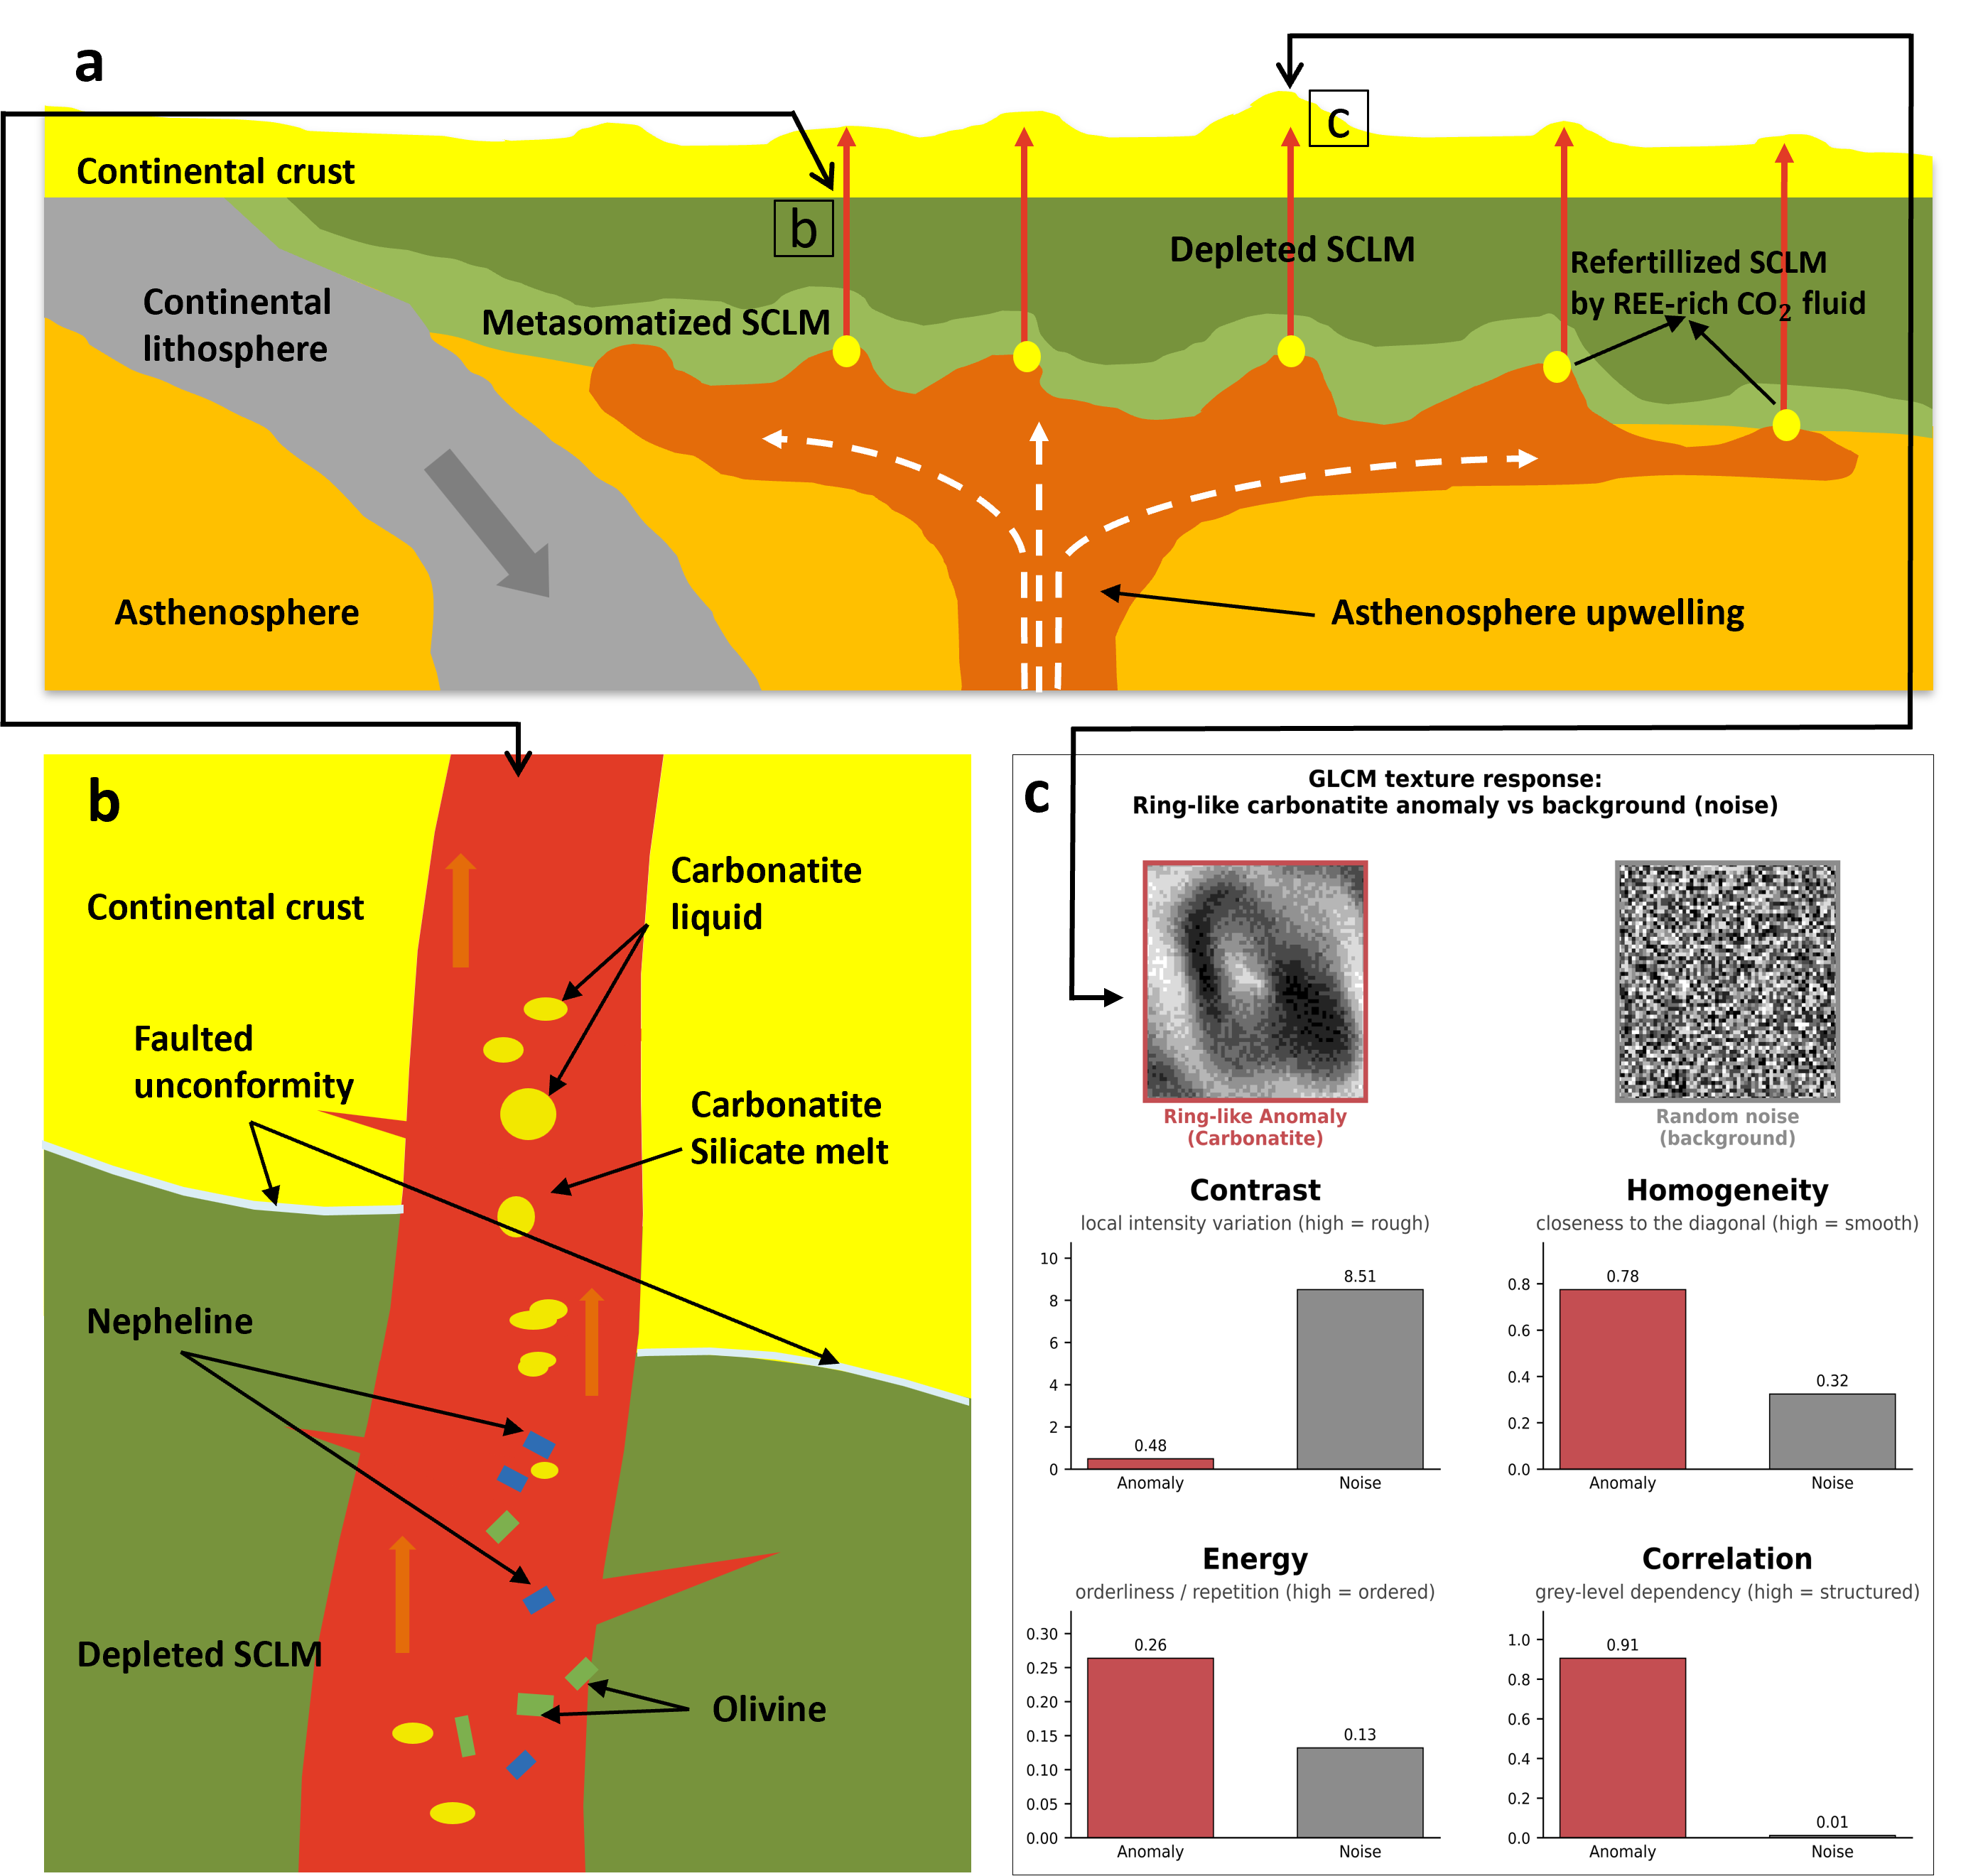
\includegraphics[width=0.85\textwidth]{figures/fig_mineral_system.png}
\caption{Source--transport--trap model for carbonatite-hosted REE systems and its geophysical proxies. (a) Source: refertilised subcontinental lithospheric mantle near the LAB at the craton margin, indexed by LAB depth and margin proximity; panel modified after \citet{Hou2023}. (b) Transport along trans-lithospheric faults, indexed by fault and worm proximity and Moho depth; modified after \citet{Yaxley2021}. (c) Trap: GLCM texture response of a ring-like anomaly and of random noise.}\label{fig:mineral-system}
\end{figure}

\subsection{Study areas}\label{sec:areas}

The three study areas are the Superior Province, the Grenville Province and the Cordilleran Orogen as outlined on the Geological Map of Canada \citep[Map 1860A;][]{Wheeler1996}. Each is modelled independently because carbonatite-hosted occurrences of the Phanerozoic, accreted Cordillera are geophysically distinct from those of the Canadian Shield \citep{Parsa2024}, so a single cross-terrane model would not be expected to transfer.

The Superior Province is the world's largest Archean craton. Carbonatite--alkaline magmatism in the Canadian Shield clusters into episodes at about 2.68~Ga, 1.90--1.88~Ga and 1.16--1.08~Ga \citep{Rukhlov2010}, and in the Superior Province many of the complexes are aligned along crustal-scale structures, most prominently the Kapuskasing Structural Zone \citep[KSZ;][]{Percival1994,Gittins1967}. The 15 Superior occurrences used here (Fig.~\ref{fig:study}b) comprise a cluster around the Montviel and Lac Shortt carbonatites in the eastern Abitibi region of Qu\'ebec (Deposit/Prospect and Showing class) and occurrences dispersed across the southern and western Superior Province, including Nemegosenda Lake, Lackner Lake, Kapuskasing, Martison Lake, Prairie Lake and Carb Lake. The Superior Province thus combines the fewest occurrences per unit area of the three provinces with a spatial structure, one tight cluster plus scattered singletons, in which a model can either learn the cluster or learn what the scattered occurrences have in common.

\begin{figure}[t]
\centering
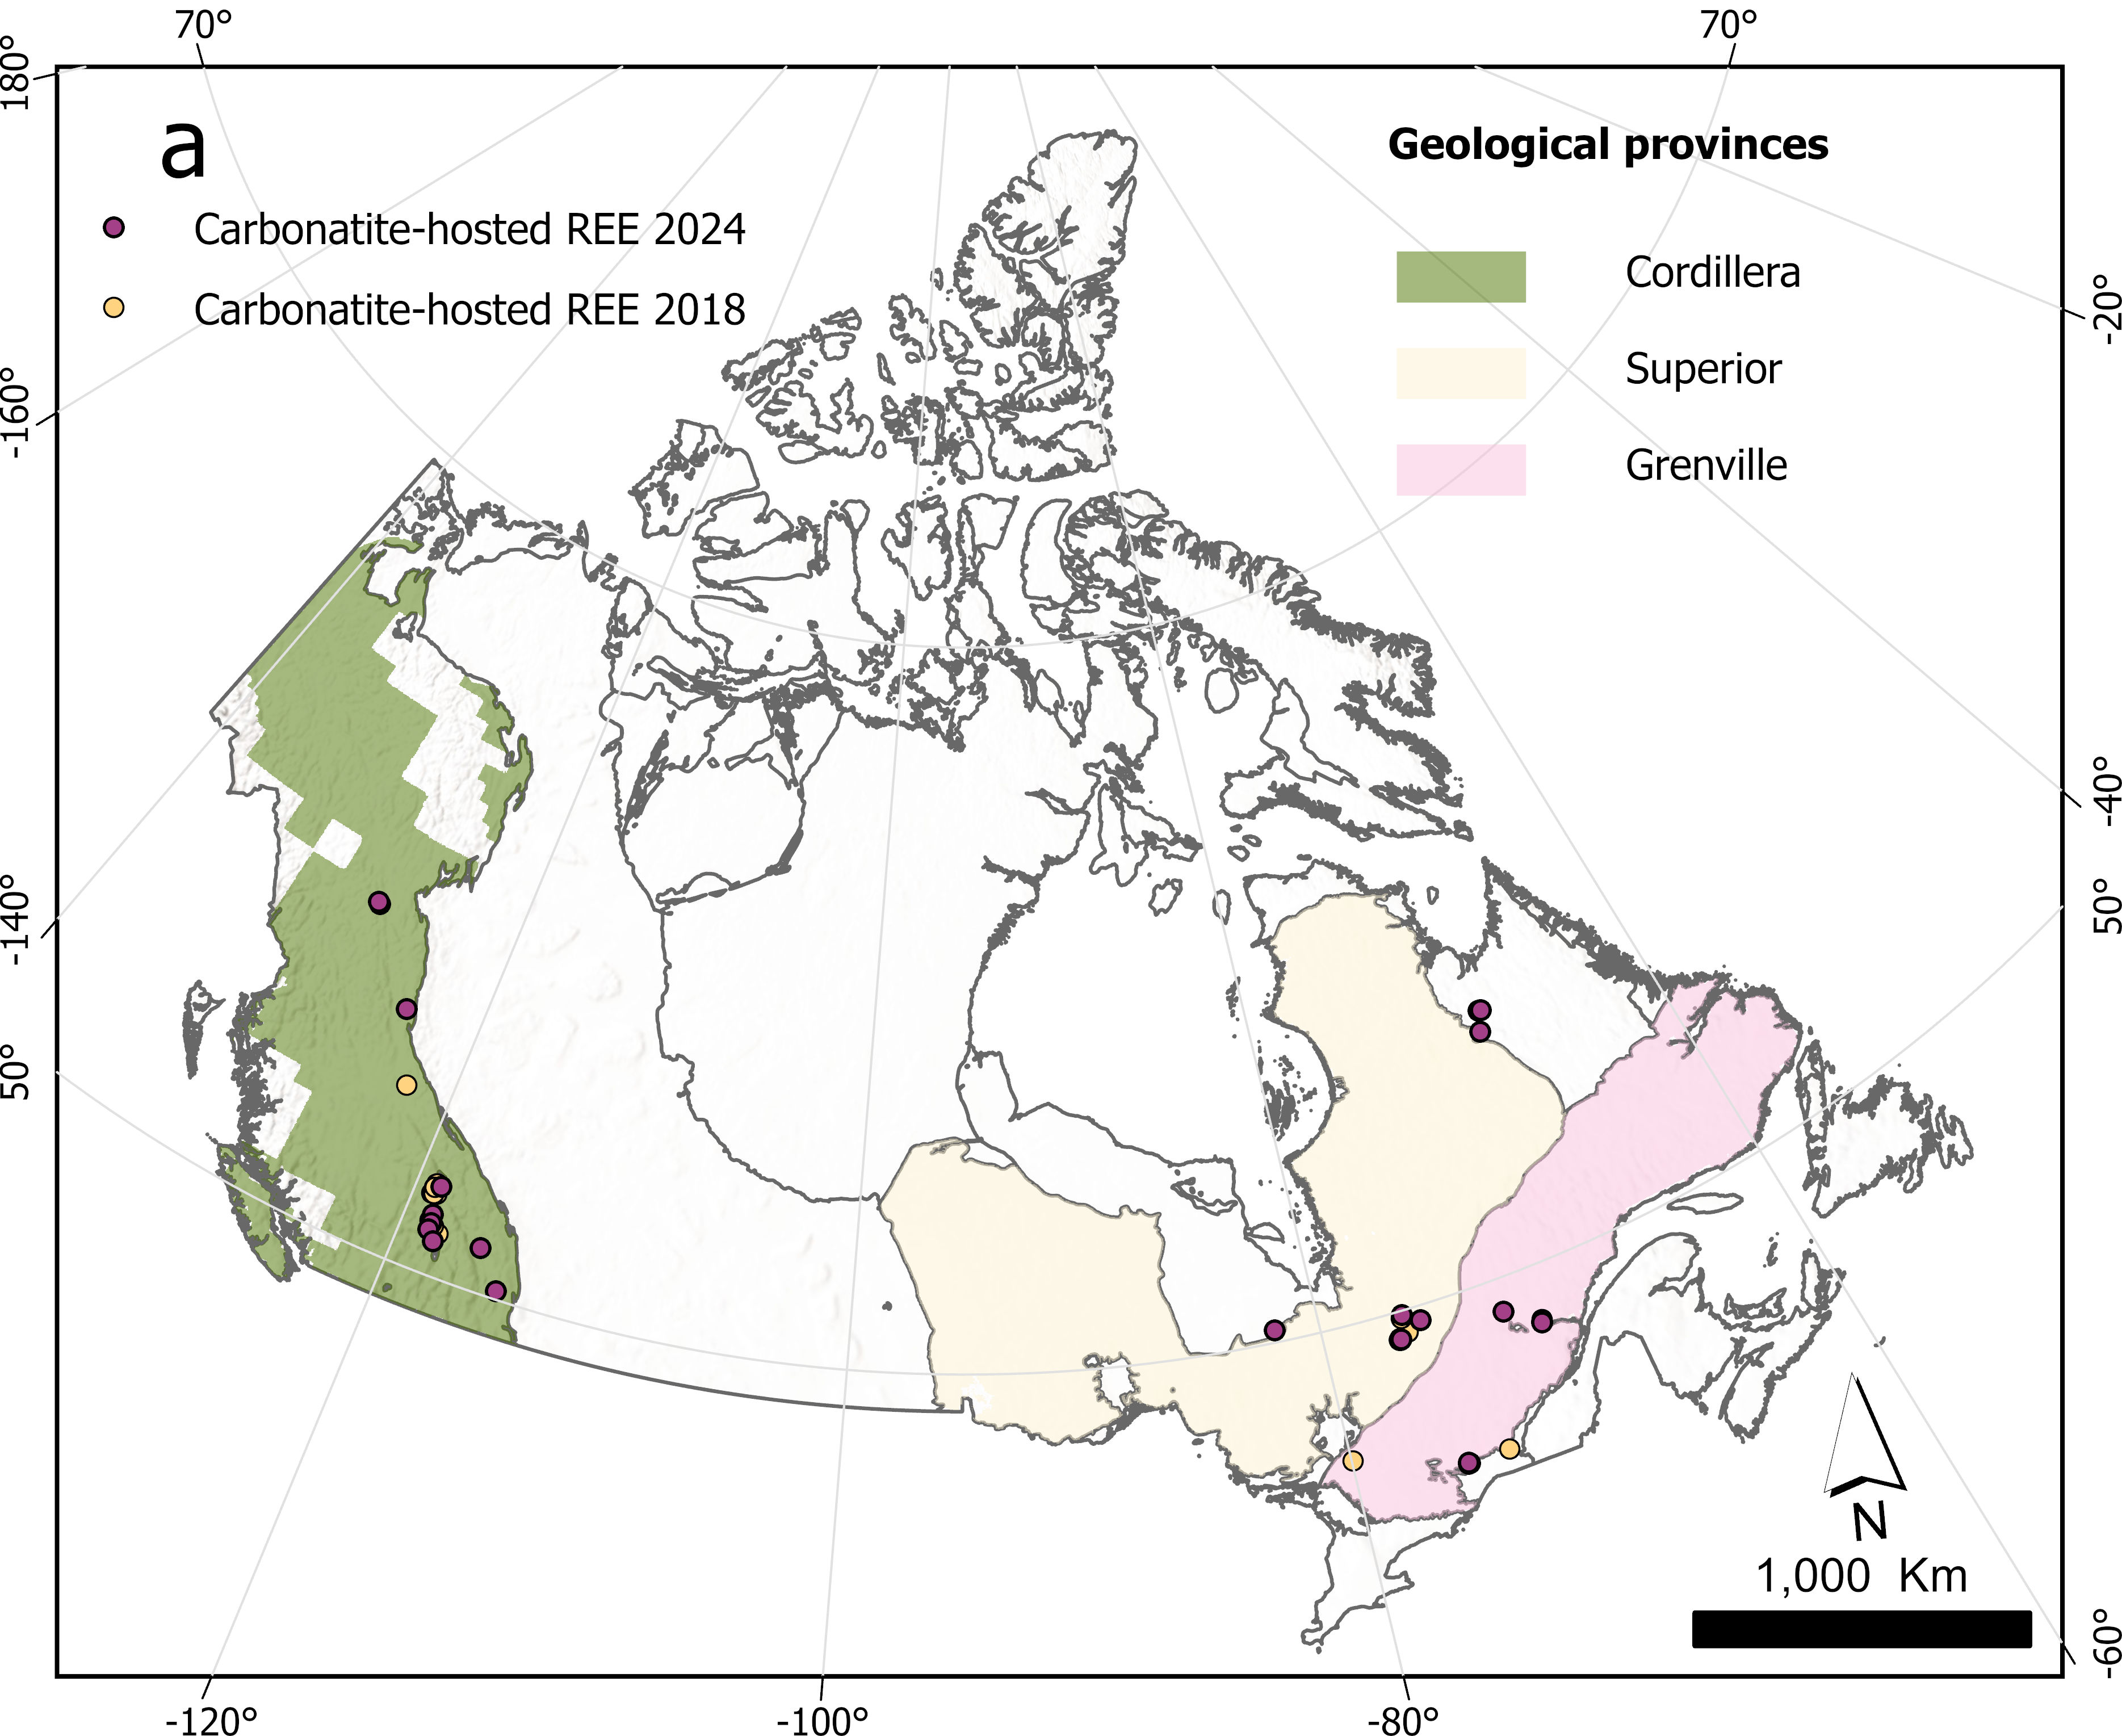
\includegraphics[width=0.55\textwidth]{figures/fig_study_canada.jpg}\hfill
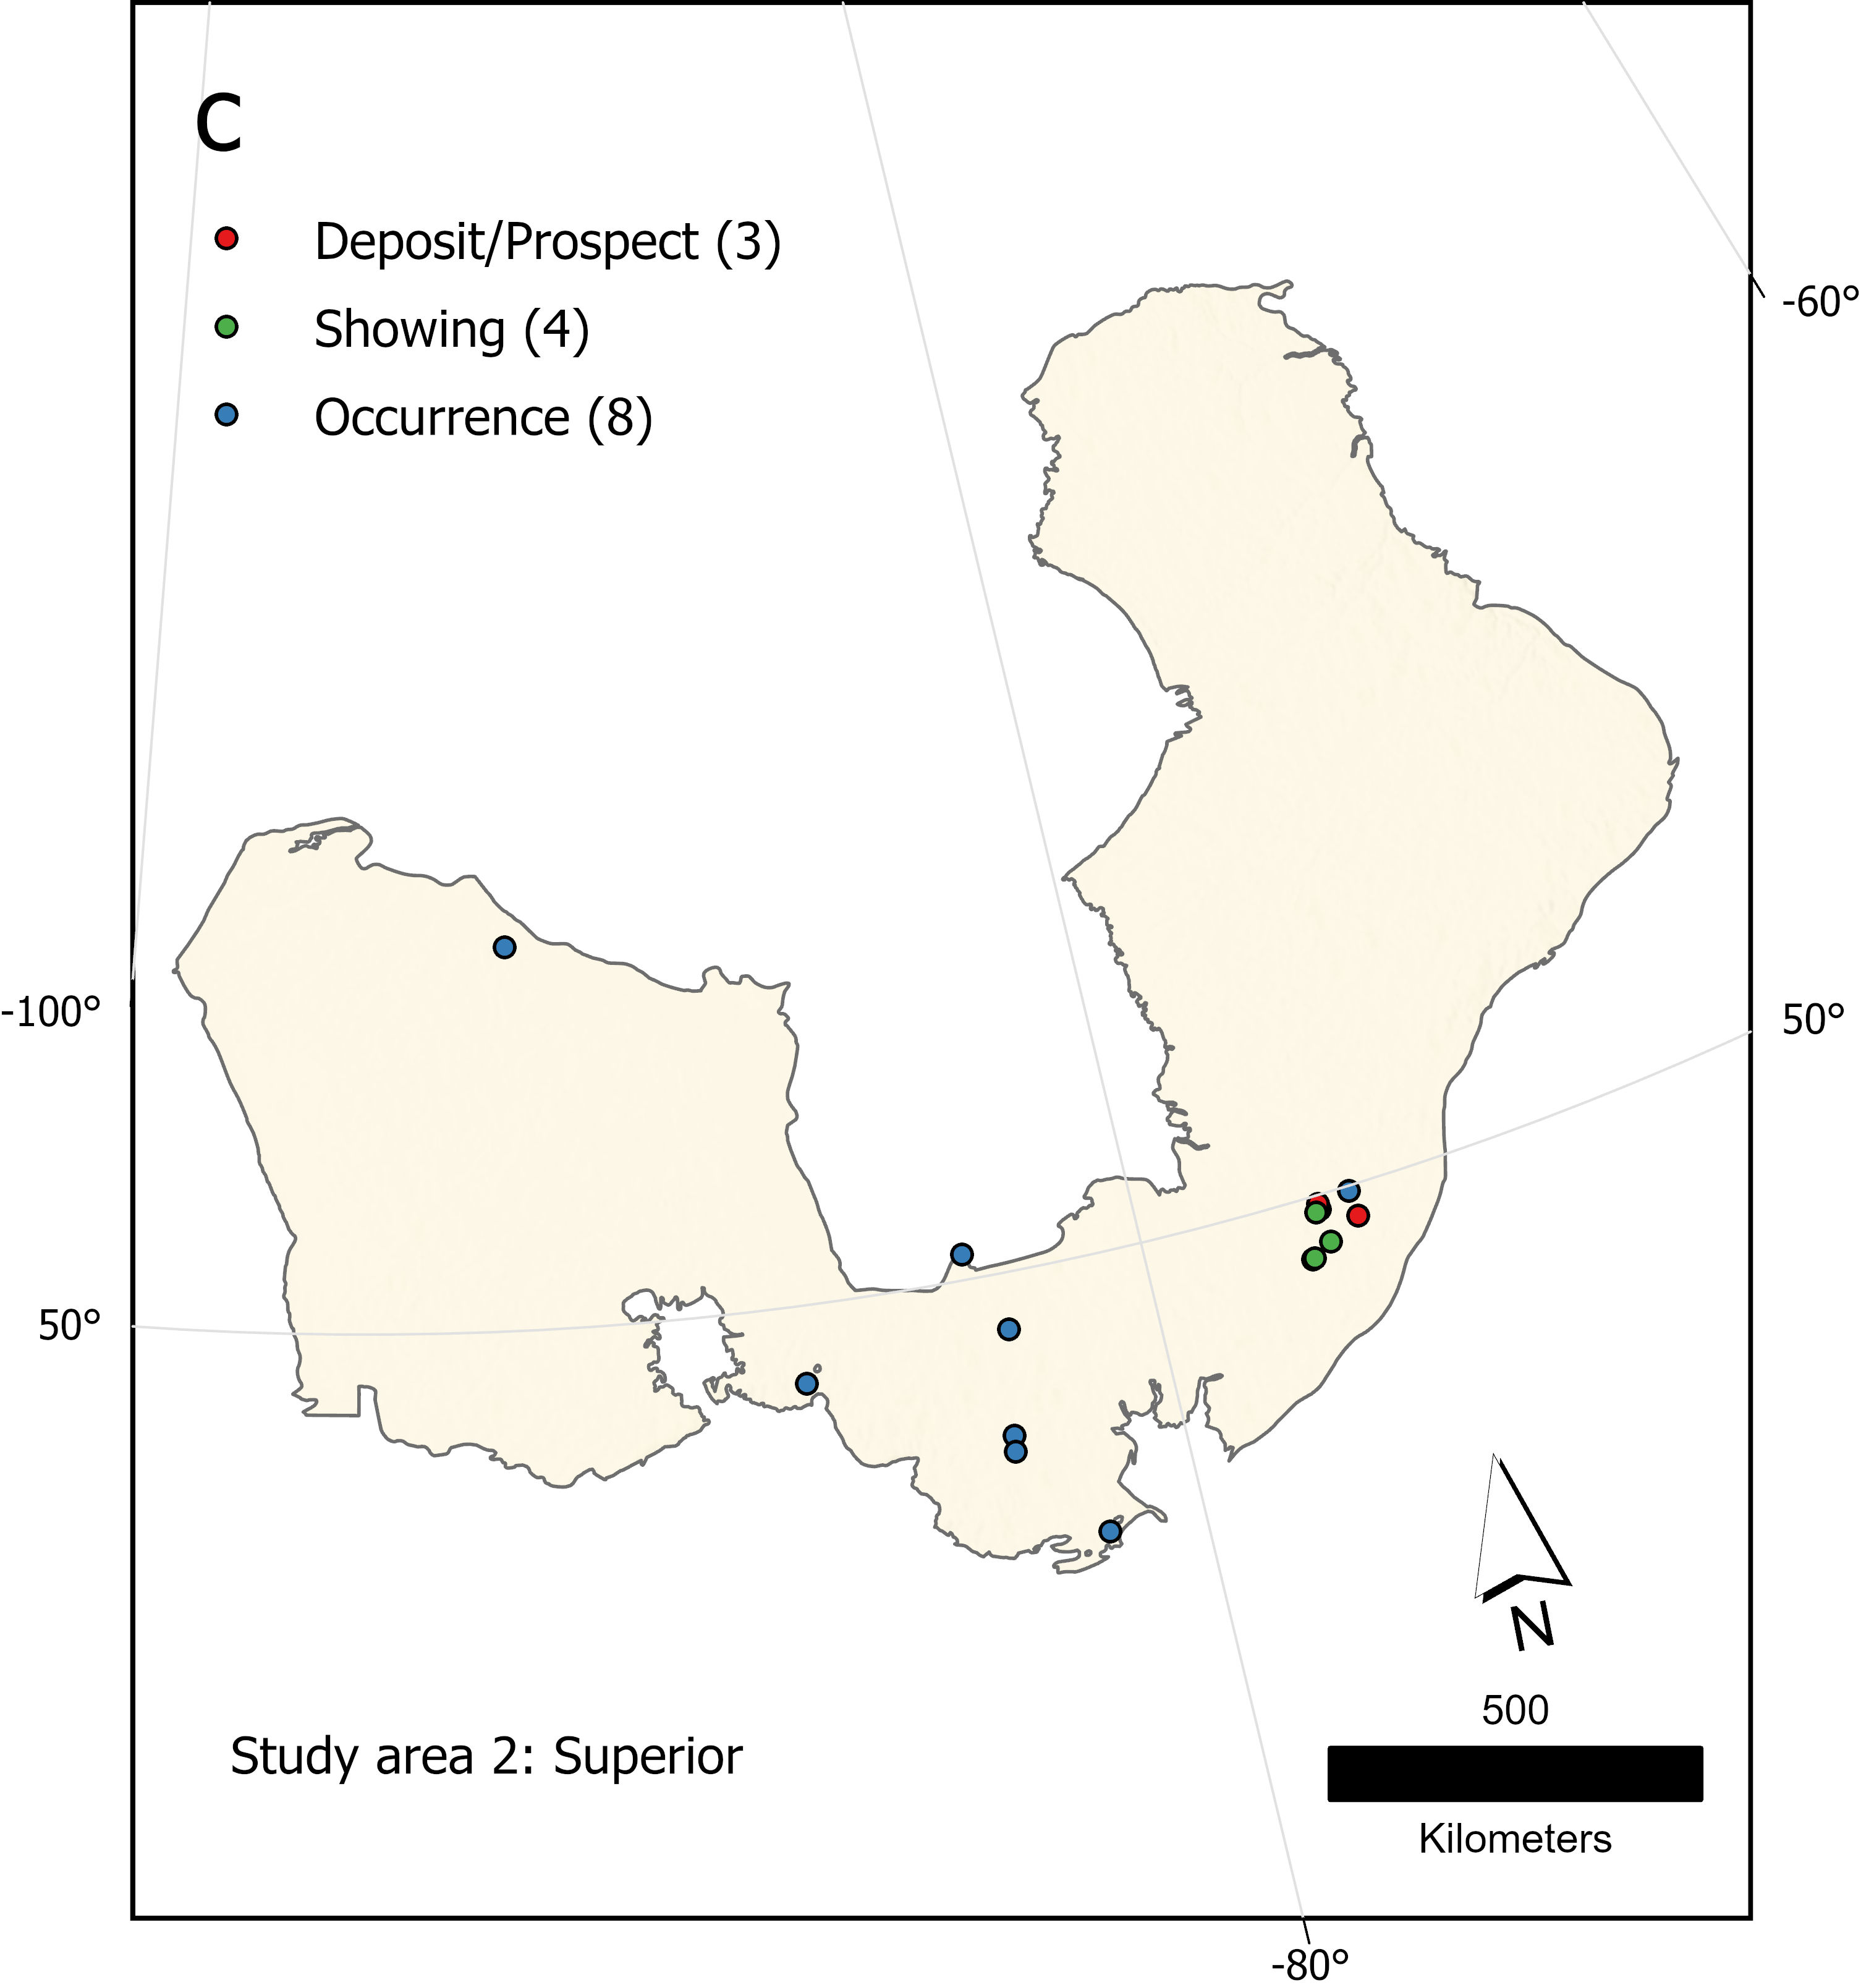
\includegraphics[width=0.42\textwidth]{figures/fig_study_superior.jpg}
\caption{(a) Carbonatite-hosted REE occurrences in Canada and the three modelled provinces; coloured areas are the sampleable domains. (b) The 15 deduplicated Superior occurrences used as positives, by development class.}\label{fig:study}
\end{figure}

\subsection{Occurrence labels}\label{sec:labels}

Positive labels were compiled from the carbonatite-hosted records of the USGS global REE occurrence database \citep{Orris2018} and the occurrence table of \citet{Parsa2024}. Alkaline-hosted occurrences were excluded after a preliminary leave-block-out classification showed them to be geophysically separable from carbonatite-hosted ones. Records within 2~km of each other were merged by single linkage, so that drill holes or zones of one deposit, listed once or in both sources, count once; without this step near-identical points from one deposit fall into both training and validation folds. Merging and the data-coverage filter (Section~\ref{sec:domain}) reduced 21, 13 and 51 pooled records to 15 (Superior), 12 (Grenville) and 27 (Cordillera) positives. Each positive keeps the development class of \citet{Parsa2024}: Deposit/Prospect, Showing or Occurrence (Superior: 3, 4 and 8).

\subsection{Evidence layers}\label{sec:layers}

Table~\ref{tab:layers} lists the evidence layers. Seventeen national rasters cover the trap and the deep-architecture components: Bouguer gravity and its derivatives and filtered versions, total magnetic intensity and its differential reduction to the pole with derivatives \citep{Jobin2017,Miles2016}, together with long-wavelength gravity and magnetics, LAB and Moho depth from the Tri-National Critical Minerals Mapping Initiative release \citep{McCafferty2023}. Eleven of the gravity and magnetic grids are processed products supplied by Getech Group plc; four of these are gridded versions of the public Natural Resources Canada compilations and seven are standard derivatives of them (Table~\ref{tab:layers}). Two line layers (ancient passive margins, \citealp{BradleyDC2008}; faults) and four point layers (shallow and deep gravity and magnetic worms; \citealp{McCafferty2023}) enter as normalised proximities, and geological era and a four-class lithology grouping are taken from an H3 (resolution 7) hexagonal grid attributed from \citet{Wheeler1996}. GLCM contrast, homogeneity, energy and correlation were computed in 9$\times$9-pixel windows on the Bouguer anomaly, its 40~km high-pass, the reduced-to-pole magnetics and the total magnetic intensity. In total each point carries 48 candidate features. Whole-rock geochemistry was not used because its coverage is too sparse to give a value at every map cell. The province polygons of \citet{Wheeler1996} define the study areas only; no distance-to-province-boundary feature was used.

\begin{table}[t]
\caption{Evidence layers, grouped by mineral-system component. Native resolution in brackets. All rasters were sampled at points in their native projection and resolution.}\label{tab:layers}
\footnotesize
\begin{tabular*}{\textwidth}{@{\extracolsep\fill}p{2.4cm}p{5.6cm}p{3.5cm}}
\toprule
Component & Layer(s) & Source \\
\midrule
Source / lithosphere & Depth to LAB (0.1$^\circ$); Moho depth (0.25$^\circ$) & \citet{McCafferty2023} \\
Deep architecture & Bouguer gravity upward-continued 30~km and its horizontal-gradient magnitude (HGM) (0.031$^\circ$); long-wavelength (deep-source) RTP magnetics and its HGM (0.02$^\circ$) & \citet{McCafferty2023} \\
%% TODO(author): confirm the provenance of the fault compilation (KNOWN_ISSUES.md #3)
Transport & Proximity to faults; to ancient passive margins; to shallow and deep gravity and magnetic worms & \citet{McCafferty2023}; \citet{BradleyDC2008} \\
Trap: gravity & Bouguer anomaly (BA), BA first vertical derivative, BA total horizontal derivative (THD) (2~km) & \citet{Jobin2017}; gridded by Getech \\
 & BA THD tilt, BA 40~km and 100~km high-pass (4th-order Butterworth) (2~km) & Getech derivatives \\
Trap: magnetics & Total magnetic intensity (TMI) (0.01$^\circ$) & \citet{Miles2016}; gridded by Getech \\
 & Differential reduction to pole (DRTP), DRTP 1VD, DRTP THD, DRTP THD tilt (0.01$^\circ$) & Getech derivatives \\
Anomaly form & GLCM contrast, homogeneity, energy, correlation (9$\times$9 window) on BA, BA 40~km high-pass, DRTP, TMI & this study \\
Host terrane & Geological era (5 classes) and lithology (4 classes), one-hot, H3 resolution 7 & \citet{Wheeler1996} \\
\botrule
\end{tabular*}
\end{table}

\subsection{Sampleable domain and background}\label{sec:domain}

Rasters were clipped to each study-area outline buffered outward by one GLCM window radius (8~km), so that windows near the boundary read real data, and sampling and prediction were restricted to the domain where every layer holds data and every texture window is computable. This domain covers 98.6\% of the Superior, 97.2\% of the Grenville and 73.5\% of the Cordilleran outline; one Cordilleran occurrence (Lempriere) falls outside it and was dropped. Background candidates are the nodes of a 0.1$^\circ$ grid inside the domain and more than 10~km from any known occurrence (19,371 in Superior). From these, two disjoint pools were drawn once per region at random: an evaluation background of 3,000 points and a training background of 5,000 points. Every model in this study is trained on the positives of its training fold plus the same 5,000 training-background points and scored on the held-out positives plus the same evaluation background. The prevalence in the scored pool is therefore 15/3,015 $\approx$ 0.5\% in Superior, which is the AP of a random ranking.

%% ===================================================================
\section{Methods}\label{sec:methods}

Figure~\ref{fig:workflow} summarises the workflow. Code for every analysis, including the exact numbers in every table, is available in the repository listed under Code availability.

\begin{figure}[t]
\centering
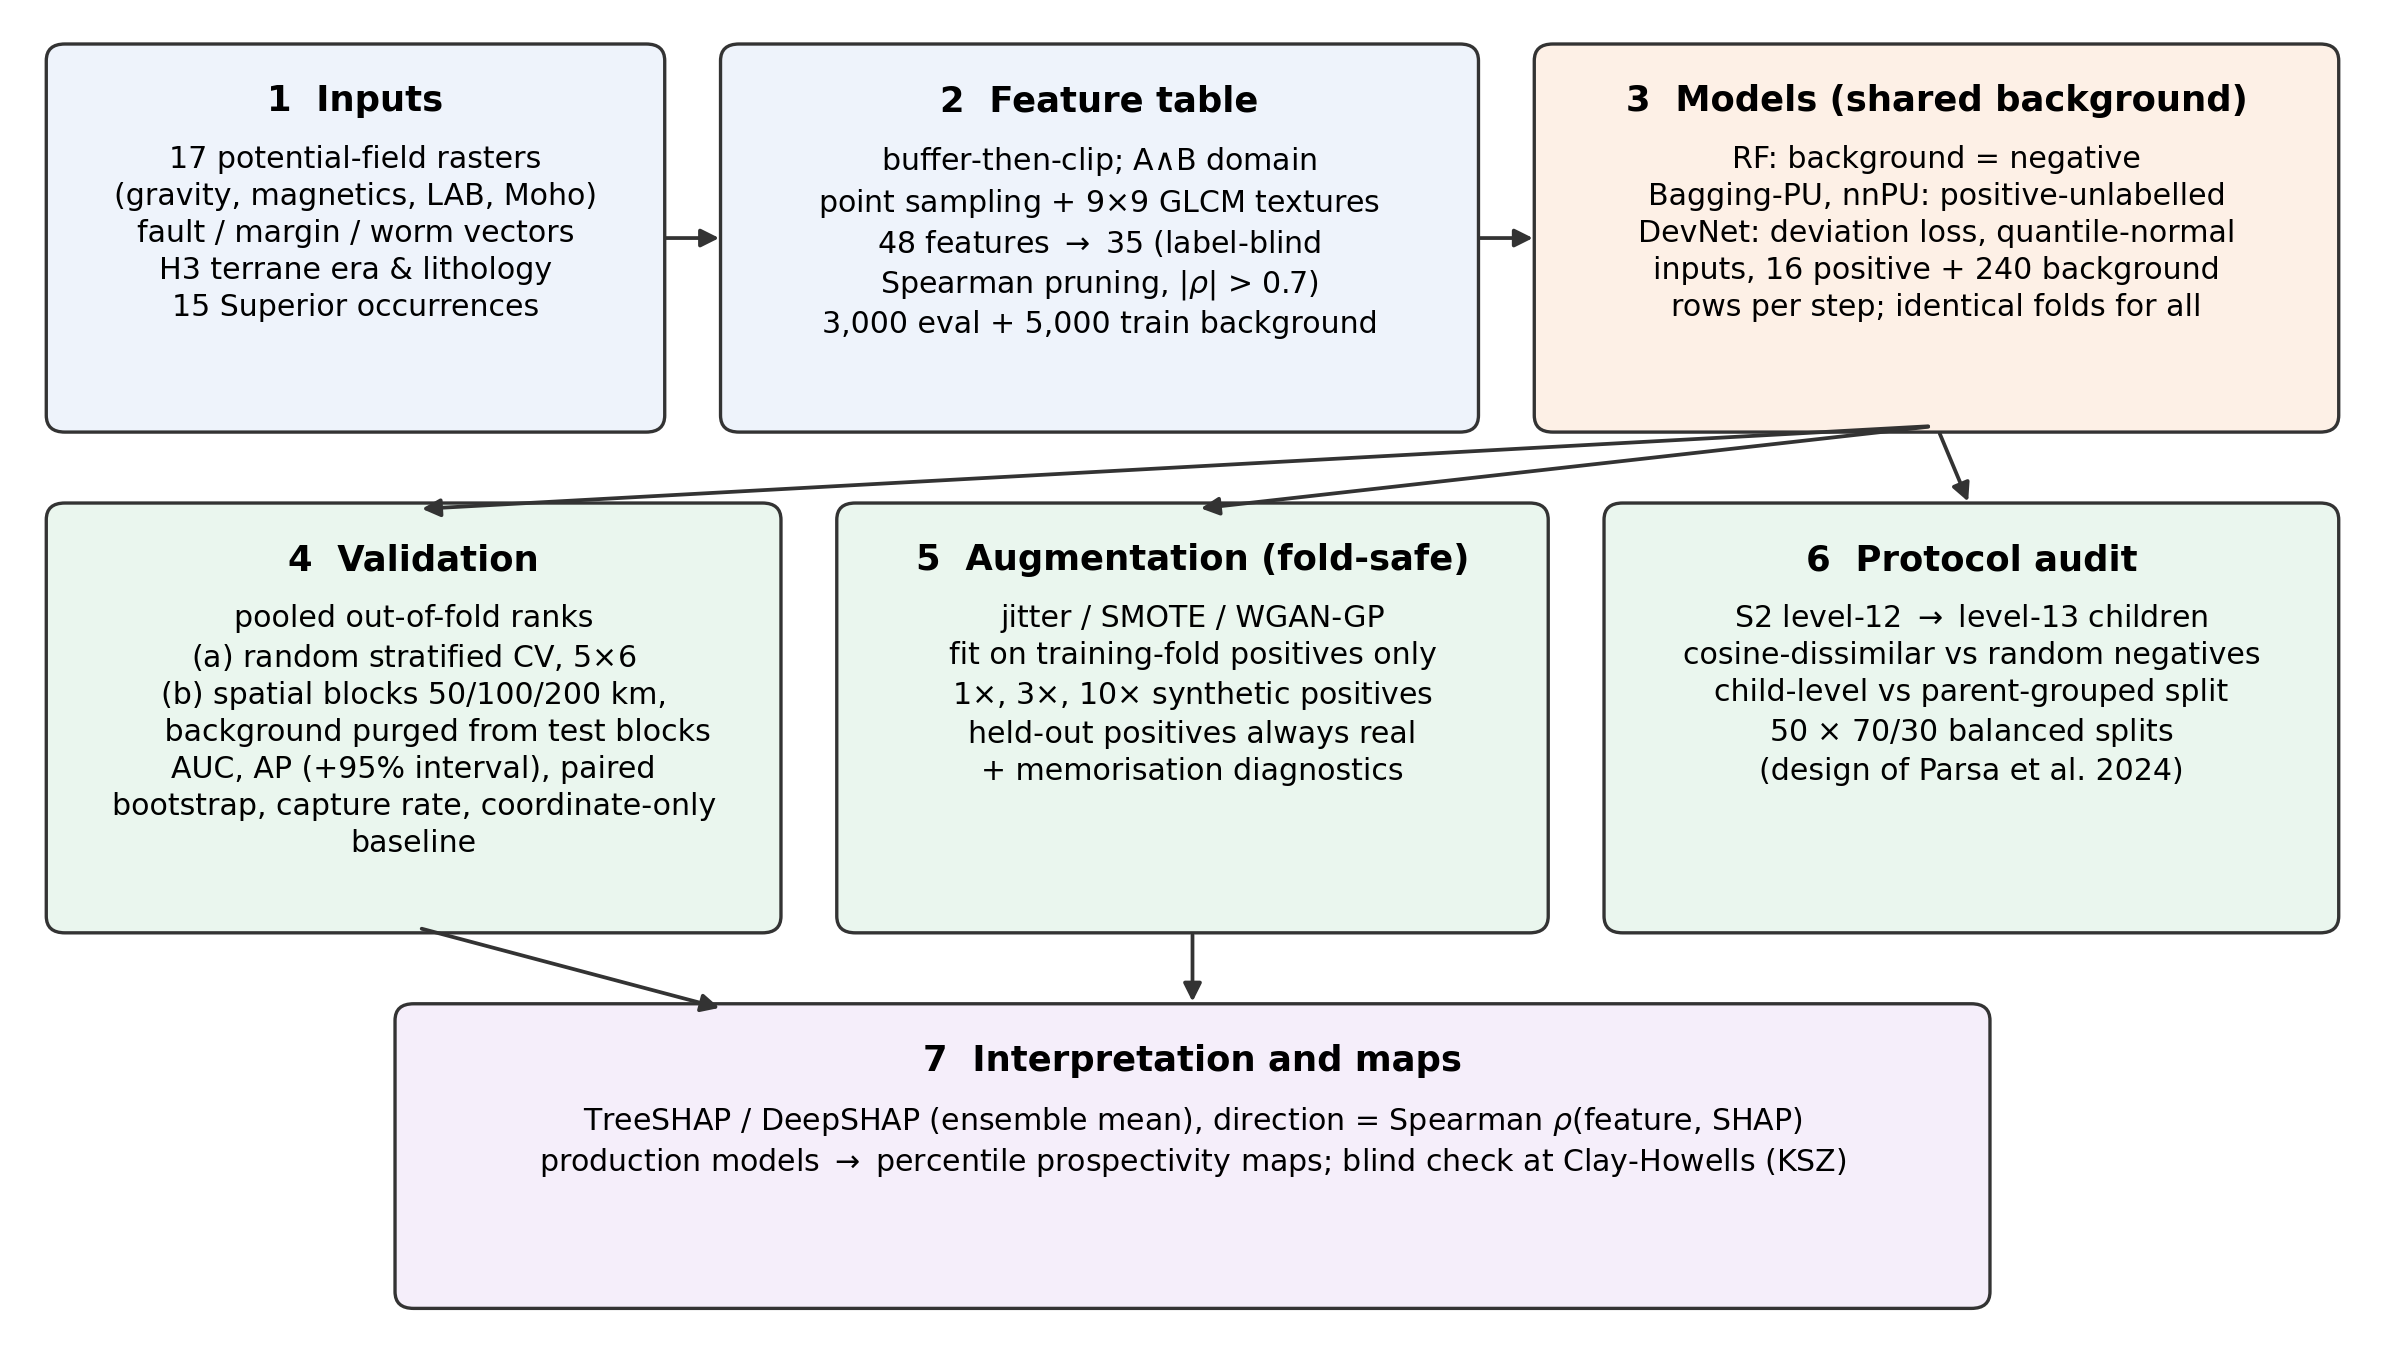
\includegraphics[width=\textwidth]{figures/fig_workflow_rev.png}
\caption{Workflow. All models are trained on the same positives and the same 5,000 background points and scored on the same folds; only the treatment of the background differs.}\label{fig:workflow}
\end{figure}

\subsection{Feature pruning}\label{sec:pruning}

The 48 features include many collinear geophysical derivatives. Within each region, features were clustered hierarchically on $1-|\rho_{\mathrm{S}}|$ (Spearman correlation, average linkage) and cut at $|\rho_{\mathrm{S}}| = 0.7$, keeping one representative per cluster chosen by lowest missing rate and then highest variance \citep{Dormann2013}. The rule never sees labels and therefore cannot leak information across folds. It leaves 35 features in Superior and 33 in Cordillera and Grenville; this pruned set is the primary feature set, and results for the full set are given in Appendix~\ref{app:full}.

\subsection{Models}\label{sec:models}

All models see the same rows and differ only in how they treat the training background.

\textbf{Random Forest} (RF; \citealp{Breiman2001}) is the discriminative baseline: positives versus training background labelled 0, 300 trees, $\sqrt{p}$ features per split, balanced class weights, inside a pipeline that fits median imputation and standardisation on the training fold only. With roughly 12 training positives against 5,000 background points, most held-out points receive a predicted probability of exactly zero (82\% of the Superior evaluation background and 2 of 15 held-out positives in one representative split), so the pooled AUC depends on which trees happen to vote for a given held-out occurrence. Changing only the RF random seed moved the single-split Superior AUC between 0.889 and 0.985 while AP varied far less (0.19--0.29). We therefore vary the RF seed across folds so that this variance enters the reported intervals, and report a single fixed seed alongside.

\textbf{DevNet} \citep{Pang2019} maps each input vector $\mathbf{x}$ to a scalar score $\phi(\mathbf{x})$ through one hidden ReLU layer with dropout. The deviation $d(\mathbf{x}) = (\phi(\mathbf{x}) - \mu_R)/\sigma_R$ is measured against the mean and standard deviation of a fixed reference sample of 50,000 standard-normal draws, and the loss
\begin{equation}
L = (1-y)\,|d(\mathbf{x})| + y\,\max\{0,\, a - d(\mathbf{x})\}
\end{equation}
pulls unlabelled background ($y=0$) towards the reference and pushes positives ($y=1$) beyond a margin $a = 5$. A sensitivity analysis over $a \in \{2,3,5,8\}$ changed Superior AP by less than 0.01; in Cordillera and Grenville smaller margins gave somewhat higher random-split AP (Appendix~\ref{app:sensitivity}, Table~\ref{tab:margin}), but we keep the value of \citet{Pang2019} rather than tune it. Network capacity was set a priori by positive count (64 hidden units, dropout 0.3, weight decay $10^{-4}$ in Cordillera; 32, 0.4 and $10^{-3}$ in Superior and Grenville) rather than tuned, because a search over a few tens of positives fits noise. Training uses Adam \citep{Kingma2014} with weight decay, cosine learning-rate annealing over 300 steps and gradient clipping, and each fold score is the rank average of five restarts with different seeds.

Two design choices adapt DevNet to tabular evidence layers with very few positives. First, inputs are mapped to standard-normal marginals by a quantile transformation fitted on each training fold. Many evidence layers are strongly skewed (inverted distances concentrated near 0 or 1, long-tailed textures, 0/1 dummies), and unlike tree ensembles, which are invariant to monotone transformations, multilayer perceptrons are sensitive to such marginal distributions \citep{Gorishniy2021,Grinsztajn2022}. Second, each gradient step uses 16 positives (resampled with replacement) and 240 background rows. The deviation loss is meant to learn what the background looks like; with label-balanced batches of 16 + 16 rows, 300 steps would show each background row about once and each positive about 400 times, whereas background-heavy batches show each background row about 14 times while positive exposure is unchanged. Appendix~\ref{app:sensitivity} reports an ablation of both choices and of the training length.

\textbf{Bagging-PU} \citep{Mordelet2014} trains 200 fully grown decision trees, each on all training positives and an equal-sized bootstrap sample of the unlabelled background, and averages their outputs. It is the standard tree-based PU learner and the closest PU analogue of RF.

\textbf{nnPU} \citep{Kiryo2017} minimises the non-negative PU risk with the sigmoid loss, using exactly DevNet's network, quantile-normal inputs, optimiser, number of steps and five-restart ensemble, so that DevNet versus nnPU isolates the loss function. nnPU requires the class prior $\pi = P(y=1)$ in the unlabelled population; we use $\pi = 0.01$ and report $\pi \in \{0.005, 0.02, 0.05\}$ for Superior. The widely used calibration approach of \citet{Elkan2008} is not included because under its assumptions the calibrated output is a monotone transform of the positive-versus-background classifier, so its ranking, and every rank metric reported here, equals RF's.

\subsection{Evaluation protocol}\label{sec:protocol}

With three or four positives per validation fold, per-fold AUC is unstable and can be undefined, so out-of-fold scores are pooled \citep{BradleyAP1997}: each held-out point is scored once per repeat, scores are converted to within-fold percentile ranks so that folds are comparable, and a single AUC and average precision (AP) are computed over all folds. Pooling carries a small known negative bias in AUC \citep{Airola2019,Parker2007}. We emphasise AP because, at 0.5\% prevalence, it reflects the practical task of concentrating occurrences into a small search area, whereas AUC is dominated by the bulk of easily rejected background \citep{Saito2015}. Exploration efficiency is also shown as capture-rate curves: the share of held-out occurrences ranked within a given top fraction of the scored pool \citep{Chung2003,Agterberg2005}. Because the evaluation background is a random sample of the domain, this fraction approximates search area. Because unexplored background may host undiscovered occurrences, all metrics are conservative.

\textbf{Random cross-validation.} Repeated stratified 5-fold cross-validation with six repeats gives six pooled AUC and AP values per model, reported as the median and the 2.5--97.5 percentile interval over repeats (labelled 95\% interval). Across the six splits the Superior DevNet AP ranges from 0.27 to 0.46 with nothing else changed, which is why a single split cannot carry a model comparison. All models use identical splits, so they can be compared pairwise.

\textbf{Spatially blocked cross-validation.} Random folds can hold out an occurrence a few kilometres from a training occurrence. Following \citet{Roberts2017} and \citet{Valavi2019}, labelled points were assigned to square blocks of 50, 100 or 200~km side in Canada Atlas Lambert (EPSG:3978), whole blocks were held out together using stratified group 5-fold splitting (fewer folds if fewer blocks contain positives), and every training-background point falling inside a held-out block was removed from training for that fold. Each of six repeats uses a random offset of the block grid.

\textbf{Paired comparisons.} For each pair of models we average each point's out-of-fold rank over the six repeats and draw 5,000 stratified bootstrap resamples of positives and background \citep{Efron1993}, reporting the difference in AP and AUC with its 95\% percentile interval, the one-sided proportion of resamples in which the difference is $\leq 0$ (denoted $p$), and the number of the six repeats in which the first model has the higher AP. With 12--27 positives these tests have little power. For the family of spatially blocked comparisons in Superior we also report $p$ values adjusted with Holm's procedure \citep{Holm1979}; elsewhere the nominal $p$ values should be read as descriptive. Averaging ranks over repeats also acts as a small ensemble, which can interact with the quantity being compared; for the augmentation experiments, where this matters, we therefore report the paired per-repeat AP difference on identical folds instead.

\textbf{Geography-only and smooth baselines.} To separate geological signal from spatial memorisation, an RF was trained on the projected coordinates of each point only, with no evidence layer, under the same folds and both protocols. Its score measures how much of a protocol's reported skill can be obtained simply by remembering where the training occurrences lie. An L2-regularised logistic regression with balanced class weights on the pruned features serves as a smooth, essentially linear discriminative reference for DevNet.

\subsection{Controls and robustness analyses}\label{sec:robust-methods}

\textbf{Supervised and tuned controls.} Two kinds of control test whether DevNet's position depends on its loss or on the attention its design received. MLP-BCE uses DevNet's network, quantile-normal inputs, batches of 16 positives and 240 background rows, 300 steps and five-restart ensemble, but replaces the deviation loss by binary cross-entropy with the background labelled 0, so DevNet versus MLP-BCE isolates the semi-supervised loss from everything else. RF-tuned and HGB-tuned give the tree-based baselines a design search of their own. Inside every outer training fold, an inner spatially blocked cross-validation (100~km blocks, three folds, training background purged from inner validation blocks) chooses the RF's minimum leaf size (1 or 10) and number of features per split ($\sqrt{p}$ or $p/3$), or the number of leaves (8 or 31) and minimum leaf size (5 or 40) of a histogram gradient-boosting classifier \citep{Pedregosa2011} with balanced class weights, 200 iterations, learning rate 0.05 and an L2 penalty of 1. The outer test fold is never used for the choice.

\textbf{Nested design selection.} DevNet's input transformation and batch composition were settled with diagnostic runs on these three provinces (Appendix~\ref{app:sensitivity}), so its scores may carry selection optimism. To measure it, the choice among the four combinations of z-scored or quantile-normal inputs and 16 or 240 background rows per step was made inside every outer training fold by the same inner spatial cross-validation (two restarts per candidate), and the chosen design, refitted on the whole outer training fold, scored the outer test fold. The resulting AP estimates what the procedure ``choose among these designs by spatial cross-validation'' achieves on unseen blocks, and its difference from the final DevNet is the optimism of having made the choice with the test folds in view.

\textbf{Feature subsets.} The terrane dummies can encode the target, because an alkaline complex mapped at a known carbonatite is close to a label, and eleven layers derive from licensed grids. DevNet and RF were therefore re-evaluated without the era and lithology dummies (27 features in Superior, 25 in Cordillera and Grenville), and with only the layers that do not derive from the licensed grids, namely the lithosphere, deep-source potential-field, proximity and terrane layers (19 features).

\textbf{Per-occurrence analysis and map stability.} To see which occurrences carry the Superior results, each positive's out-of-fold percentile among the evaluation background was averaged over the six repeats and compared between the eastern-Abitibi cluster (the eight occurrences joined to Montviel by single linkage at 50~km) and the seven dispersed occurrences. Prediction--area curves \citep{YousefiCarranza2015} were computed from the same out-of-fold ranks, with the evaluation background as a proxy for area. To assess the stability of the maps, each Superior occurrence was left out in turn and the production DevNet and RF were refitted on the other 14; for every grid node we report the share of these 15 models that place it in the province's top 5\%.

\textbf{Province diagnostics.} To describe, independently of any model, why skill differs between provinces, each label set was characterised by its number of independent sites (occurrences merged by single linkage at 10~km), the share of occurrences that share a site with another and the median distance to the nearest other occurrence. The signal shared by distant occurrences was measured with a far-neighbour index: with features expressed as percentile ranks, it is, for each occurrence, the share of background points more than 100~km away that are closer to it in feature space than the most similar occurrence more than 100~km away. A value near 0 means that distant occurrences resemble one another more than they resemble almost any background. The median over occurrences, computed on the geophysical and structural features, is compared with the same statistic for 200 sets of background points drawn at random to pose as occurrences.

\subsection{Synthetic positives}\label{sec:augmentation}

To test whether synthetic positives can compensate for label scarcity, each training fold's real positives were augmented with $m \times n_{\mathrm{pos}}$ synthetic positives ($m = 1, 3, 10$) before RF and DevNet were retrained; the held-out positives were always real. Three generators were compared, all fitted in the standardised feature space of the training fold only: Gaussian jitter of real positives ($\sigma = 0.1$ standard deviations); SMOTE-style interpolation between a positive and one of its three nearest positive neighbours \citep{Chawla2002}; and a tabular Wasserstein GAN with gradient penalty \citep[WGAN-GP;][]{Goodfellow2014,Arjovsky2017,Gulrajani2017} with an eight-dimensional latent input, two hidden layers of 64 units in generator and critic, five critic updates per generator update, gradient-penalty weight 10 and 2,000 generator updates, trained on the fold's 12 positives. Synthetic terrane dummies were snapped back to valid one-hot values. To see what the generators produce, each was also fitted to all 15 Superior positives and 150 samples were characterised by the distance to the nearest real positive divided by the median nearest-neighbour distance among real positives (a value near 0 indicates copying), by the share of samples whose nearest labelled neighbour is a positive rather than a background point, and by their DevNet score percentile.

\subsection{Validation-protocol audit}\label{sec:audit-methods}

To quantify how the validation design of \citet{Parsa2024} behaves on these data, we rebuilt it with the same S2 geometry library. Each occurrence's level-12 S2 cell (about 4.5~km$^2$) was replaced by its four level-13 child cells, and all features were extracted at the child-cell centres with the same pipeline. An equal number of negatives was drawn either from the 5\% of background candidates with the lowest mean cosine similarity to the augmented positives in min--max scaled feature space (as described by \citealp{Parsa2024}) or at random. Random forests of 1,000 trees on min--max scaled features were evaluated with 50 stratified 70/30 splits. Three split designs were compared: (i) child-level random splitting, as described in the original study; (ii) splitting with all children of one parent kept on the same side; and (iii) no augmentation, one label per occurrence. We report mean test AUC, its 2.5--97.5 percentile range over the 50 splits, and the share of test positives with a sibling in the training set. The audit uses the full 48-feature set and our layers rather than those of the original study, so it measures the sensitivity of the protocol, not the original study's numbers.

\subsection{Interpretation and mapping}\label{sec:shap}

Production models were fitted to all positives and the training background of each region. SHAP values \citep{Lundberg2017} were computed with TreeSHAP for RF \citep{Lundberg2020} and DeepSHAP for DevNet on an explain set of all positives plus evaluation-background points (200 in total), with 100 training-background points as DevNet's reference sample; DevNet's SHAP values refer to its quantile-transformed inputs, which leaves the rank-based directions defined below unaffected. DevNet SHAP values were averaged over the five ensemble members. Importance is mean $|$SHAP$|$. The \emph{direction} of a feature's effect is the Spearman correlation between the feature's value and its SHAP value over the explain set (for one-hot dummies, the sign of the mean SHAP difference between presence and absence), with $|\rho| < 0.1$ reported as no clear direction. We do not use the sign of the mean SHAP value, a tempting summary that reflects where the explained points lie relative to the explainer's baseline, not whether higher feature values raise the score: for RF with balanced class weights the TreeSHAP baseline is near 0.5 while nearly all explained points score near 0, so that rule would label every RF feature as ``higher $\rightarrow$ less prospective''. Prospectivity maps classify each model's scores on a 0.1$^\circ$ prediction grid into the top 1\%, 5\% and 10\%, because DevNet's anomaly score and RF's probability are not on a common scale.

%% ===================================================================
\section{Results}\label{sec:results}

\subsection{Model comparison under random cross-validation}\label{sec:res-random}

In Superior all models rank held-out occurrences far above chance (Table~\ref{tab:benchmark}): AP is 0.19--0.35 against a random-ranking value of 0.005, and AUC is 0.84--0.97. DevNet has the highest median AP (0.354) and RF and bagging-PU the highest AUC (0.973 and 0.969). DevNet's AP exceeds RF's in all six repeated splits ($+0.161$, 95\% interval $[-0.064, +0.376]$, $p = 0.076$) and bagging-PU's in five ($+0.143$, $p = 0.086$; Table~\ref{tab:bootstrap}): with 15 positives, random cross-validation leaves these differences within their uncertainty. nnPU, which shares DevNet's network and inputs, attains a competitive AP (0.278) but a markedly lower AUC (0.835; $\Delta$AUC $+0.121$ in DevNet's favour, $p = 0.028$), and its AP depends on the assumed class prior (Table~\ref{tab:prior}), which is unknown in practice.

The contrasting regions behave differently. In Cordillera, RF and bagging-PU are clearly superior to DevNet (AP 0.379 and 0.340 against 0.136; DevNet's AP is lower than RF's in all six repeats, bootstrap interval of the difference $[-0.395, -0.128]$), and nnPU fails (AUC 0.57). In Grenville all models are weak and RF leads (0.265); DevNet (0.137) is level with bagging-PU (0.163), and nnPU again fails (AUC 0.60). That Superior is the best-predicted of the three provinces agrees with the province-level success rates of \citet{Parsa2024}.

\begin{table}[t]
\caption{Pooled out-of-fold AUC and AP (median and 95\% interval over six repeated 5-fold random splits; pruned features). Bold: best of the four main models in each region. RF (fixed seed): a single random seed for all folds.}\label{tab:benchmark}
\footnotesize
\begin{tabular*}{\textwidth}{@{\extracolsep\fill}llcc}
\toprule
Region ($n_{\mathrm{pos}}$) & Model & AUC & AP \\
\midrule
\multirow{5}{*}{Superior (15)} & DevNet & 0.951 [0.941, 0.962] & \textbf{0.354} [0.276, 0.453] \\
 & RF & \textbf{0.973} [0.952, 0.982] & 0.214 [0.154, 0.261] \\
 & Bagging-PU & 0.969 [0.955, 0.973] & 0.189 [0.137, 0.344] \\
 & nnPU & 0.835 [0.822, 0.839] & 0.278 [0.157, 0.306] \\
 & RF (fixed seed) & 0.957 [0.893, 0.975] & 0.220 [0.168, 0.257] \\
\midrule
\multirow{5}{*}{Cordillera (27)} & DevNet & 0.873 [0.833, 0.883] & 0.136 [0.100, 0.178] \\
 & RF & 0.904 [0.891, 0.933] & \textbf{0.379} [0.280, 0.426] \\
 & Bagging-PU & \textbf{0.912} [0.898, 0.932] & 0.340 [0.251, 0.379] \\
 & nnPU & 0.574 [0.559, 0.584] & 0.019 [0.015, 0.019] \\
 & RF (fixed seed) & 0.916 [0.909, 0.958] & 0.389 [0.291, 0.473] \\
\midrule
\multirow{5}{*}{Grenville (12)} & DevNet & 0.770 [0.676, 0.805] & 0.137 [0.053, 0.191] \\
 & RF & 0.837 [0.767, 0.858] & \textbf{0.265} [0.200, 0.382] \\
 & Bagging-PU & \textbf{0.842} [0.811, 0.861] & 0.163 [0.073, 0.231] \\
 & nnPU & 0.597 [0.571, 0.628] & 0.012 [0.009, 0.021] \\
 & RF (fixed seed) & 0.791 [0.720, 0.852] & 0.238 [0.199, 0.493] \\
\botrule
\end{tabular*}
\end{table}

\begin{table}[t]
\caption{Paired comparisons of DevNet with each other model (random cross-validation, pruned features): difference in AP and AUC computed on repeat-averaged out-of-fold ranks, with 95\% stratified bootstrap interval, one-sided $p = P(\Delta \leq 0)$, and the number of the six repeats in which DevNet has the higher AP.}\label{tab:bootstrap}
\footnotesize
\setlength{\tabcolsep}{2.5pt}
\begin{tabular*}{\textwidth}{@{\extracolsep\fill}llccccc}
\toprule
Region & Comparison & $\Delta$AP [95\%] & $p$ & AP wins & $\Delta$AUC & $p$ \\
\midrule
Superior & DevNet $-$ RF & +0.161 [-0.064, +0.376] & 0.076 & 6/6 & -0.027 & 0.885 \\
Superior & DevNet $-$ Bagging-PU & +0.143 [-0.064, +0.360] & 0.086 & 5/6 & -0.017 & 0.714 \\
Superior & DevNet $-$ nnPU & +0.073 [-0.059, +0.237] & 0.128 & 5/6 & +0.121 & 0.028 \\
\addlinespace
Cordillera & DevNet $-$ RF & -0.266 [-0.395, -0.128] & 1.000 & 0/6 & -0.056 & 0.987 \\
Cordillera & DevNet $-$ Bagging-PU & -0.202 [-0.315, -0.075] & 0.999 & 0/6 & -0.045 & 0.989 \\
Cordillera & DevNet $-$ nnPU & +0.146 [+0.072, +0.278] & 0.000 & 6/6 & +0.300 & 0.000 \\
\addlinespace
Grenville & DevNet $-$ RF & -0.166 [-0.327, -0.028] & 1.000 & 0/6 & -0.044 & 0.956 \\
Grenville & DevNet $-$ Bagging-PU & -0.014 [-0.151, +0.126] & 0.569 & 2/6 & -0.083 & 1.000 \\
Grenville & DevNet $-$ nnPU & +0.224 [+0.015, +0.471] & 0.001 & 6/6 & +0.177 & 0.029 \\
\botrule
\end{tabular*}
\end{table}

\begin{table}[t]
\caption{Sensitivity of nnPU to the assumed class prior $\pi$, Superior (random cross-validation).}\label{tab:prior}
\footnotesize
\begin{tabular*}{0.6\textwidth}{@{\extracolsep\fill}lcc}
\toprule
$\pi$ & AUC & AP \\
\midrule
0.005 & 0.806 [0.788, 0.813] & 0.207 [0.143, 0.265] \\
0.01 & 0.835 [0.822, 0.839] & 0.278 [0.157, 0.306] \\
0.02 & 0.841 [0.835, 0.843] & 0.297 [0.243, 0.331] \\
0.05 & 0.862 [0.860, 0.866] & 0.284 [0.257, 0.316] \\
\botrule
\end{tabular*}
\end{table}

\subsection{Spatially blocked validation}\label{sec:res-spatial}

Holding out whole blocks changes the picture in Superior (Fig.~\ref{fig:spatial}; Table~\ref{tab:spatial}). RF's AP falls from 0.214 under random splits to 0.128 with 50 and 100~km blocks and 0.094 with 200~km blocks, and bagging-PU follows the same path (0.110--0.122). DevNet's AP stays between 0.302 and 0.341 at every block size, and nnPU's between 0.233 and 0.236. DevNet exceeds RF in all six repeats at every block size, with paired differences of $+0.272$, $+0.245$ and $+0.298$ at 50, 100 and 200~km ($p \leq 0.008$), and it also exceeds bagging-PU at every block size ($p \leq 0.024$; Table~\ref{tab:spatial-boot}). DevNet is also ahead of nnPU in five or six of six repeats at every block size, but the difference ($+0.04$ to $+0.14$) is significant only with 50~km blocks ($p = 0.003$). With Holm's correction over these nine comparisons, the differences from RF remain significant at every block size (adjusted $p \leq 0.047$), as does the difference from nnPU with 50~km blocks (0.021), whereas those from bagging-PU do not (0.069--0.087). Capture-rate curves show the same effect (Fig.~\ref{fig:capture}). Under random splits the models capture 40--67\% of the held-out occurrences in the top 1--2\% of the ranked pool. Under 100~km blocks DevNet still captures about half of them in the top 1\%, against about a third for RF and bagging-PU, and its advantage persists to the 10\% mark.

Table~\ref{tab:occurrence} shows which occurrences carry this advantage. Under 100~km blocks DevNet places five of the seven dispersed Superior occurrences in the top 1\% of the scored pool (median percentile 0.997), against two for RF and one for bagging-PU. In the eastern-Abitibi cluster the tree-based models lose most under blocking (RF median percentile 0.981 under random splits and 0.893 under 100~km blocks), whereas DevNet changes little (0.987 and 0.976). DevNet's clearest miss is Nemegosenda Lake, which it ranks at the 56th--57th percentile under both protocols. Prediction--area curves (Appendix~\ref{app:full}, Fig.~\ref{fig:pa}), which summarise the whole ranking rather than its top, separate the models less: at the intersection point under 100~km blocks DevNet and bagging-PU capture 87\% of the held-out occurrences in the top 13\% of the area and RF 81\% in 19\%, and under random splits the three models capture 89--92\%.

\begin{table}[t]
\caption{Superior occurrences by group: median out-of-fold percentile among the evaluation background (mean over six repeats) and, in brackets, the number of occurrences ranked in the top 1\%. Abitibi cluster: the eight occurrences joined to Montviel by single linkage at 50~km.}\label{tab:occurrence}
\scriptsize
\setlength{\tabcolsep}{2.5pt}
\begin{tabular*}{\textwidth}{@{\extracolsep\fill}llccccc}
\toprule
Split & Group & DevNet & MLP-BCE & RF & Bagging-PU & nnPU \\
\midrule
\multirow{2}{*}{random} & Abitibi cluster (8) & 0.987 (2/8) & 0.981 (3/8) & 0.981 (4/8) & 0.753 (3/8) \\
 & dispersed (7) & 0.997 (5/7) & 0.975 (1/7) & 0.980 (3/7) & 0.972 (3/7) \\
\addlinespace
\multirow{2}{*}{100 km} & Abitibi cluster (8) & 0.976 (3/8) & 0.893 (2/8) & 0.932 (2/8) & 0.762 (2/8) \\
 & dispersed (7) & 0.997 (5/7) & 0.974 (2/7) & 0.965 (1/7) & 0.981 (3/7) \\
\botrule
\end{tabular*}
\end{table}

In Cordillera every model degrades sharply under blocking (AP $\leq$ 0.07 at 50~km and $\leq$ 0.03 at 100--200~km), and in Grenville AP approaches the random-ranking value. In these regions no difference between DevNet and the tree-based models is of practical size. The Cordilleran and Grenville models therefore owe much of their random-split skill to spatial proximity between training and test occurrences, whereas DevNet retains its ranking skill in Superior on ground that lies 100--200~km from any training occurrence.

\begin{figure}[t]
\centering
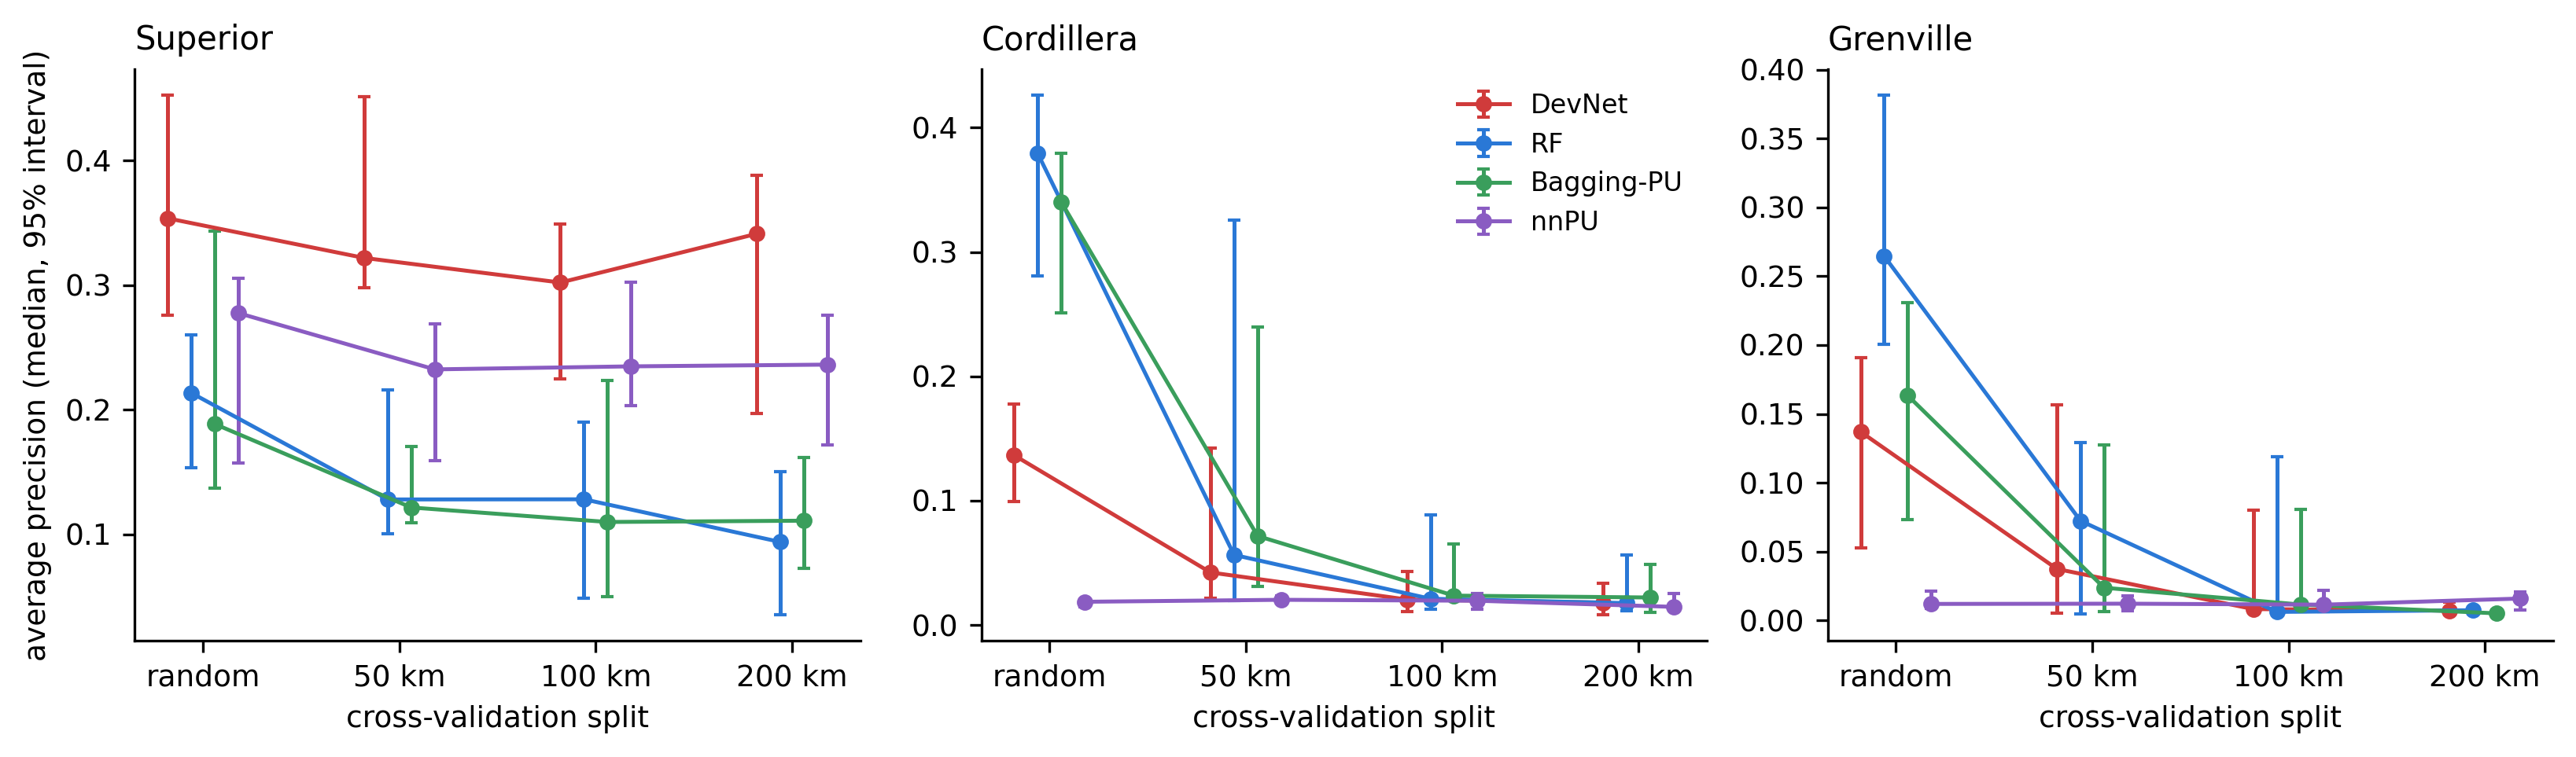
\includegraphics[width=\textwidth]{figures/fig_spatial_cv_rev.png}
\caption{Average precision under random and spatially blocked cross-validation (median and 95\% interval over six repeats). The random-ranking AP is 0.005 (Superior), 0.009 (Cordillera) and 0.004 (Grenville).}\label{fig:spatial}
\end{figure}

\begin{figure}[t]
\centering
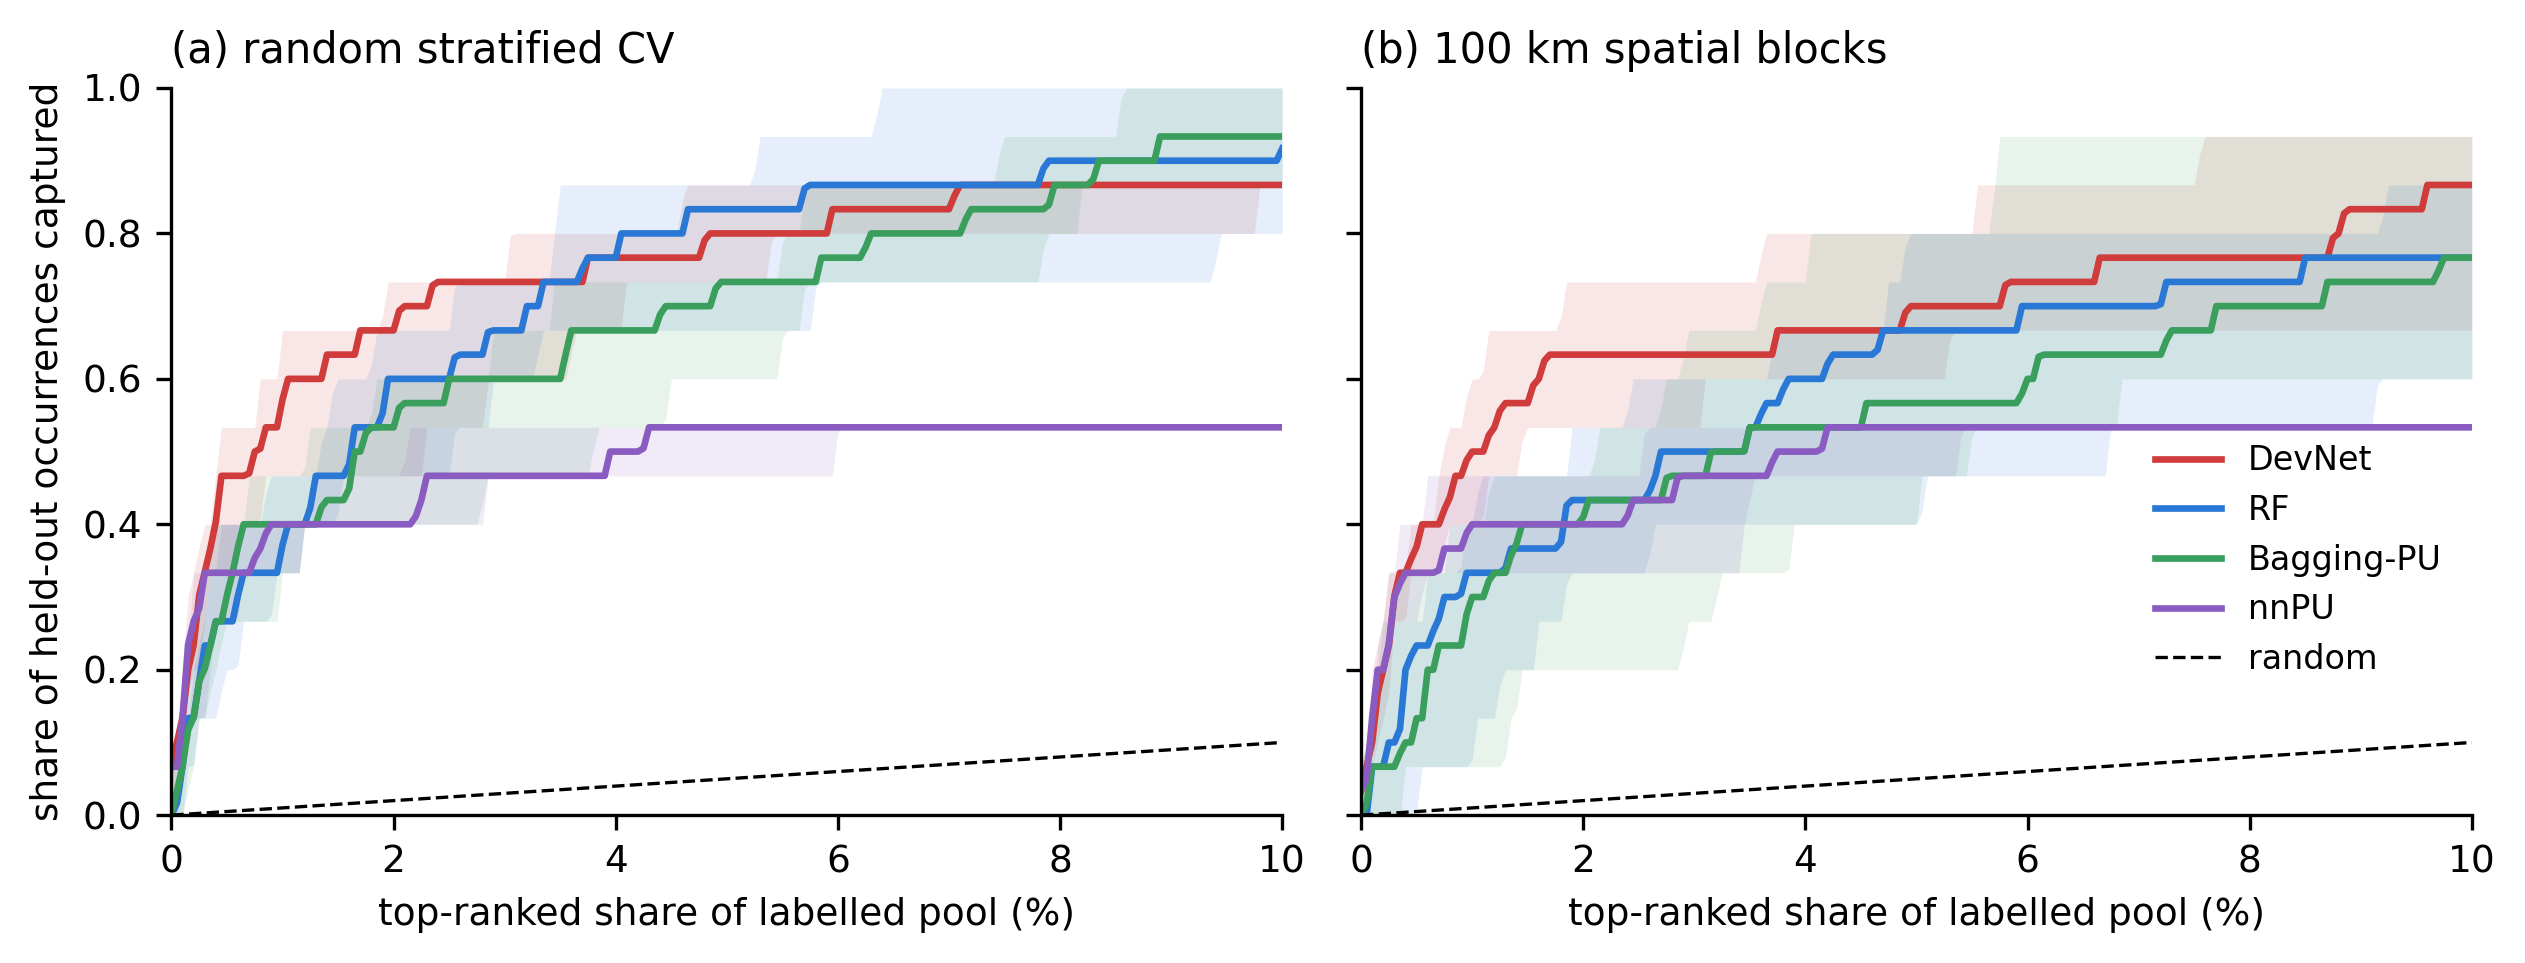
\includegraphics[width=0.9\textwidth]{figures/fig_capture_superior_rev.png}
\caption{Superior capture-rate curves: share of held-out occurrences ranked within the top fraction of the scored pool (a proxy for search area), (a) random cross-validation and (b) 100~km spatial blocks. Lines: median over six repeats; bands: range. Dashed: random ranking.}\label{fig:capture}
\end{figure}

\begin{table}[t]
\caption{Average precision (median over six repeats) under random and spatially blocked cross-validation. Bold: highest AP in each row. AUC for the same runs is given in Appendix~\ref{app:full} (Table~\ref{tab:spatial-auc}).}\label{tab:spatial}
\footnotesize
\setlength{\tabcolsep}{3pt}
\begin{tabular*}{\textwidth}{@{\extracolsep\fill}llcccc}
\toprule
Region & Split & DevNet & RF & Bagging-PU & nnPU \\
\midrule
\multirow{4}{*}{Superior} & random & \textbf{0.354} & 0.214 & 0.189 & 0.278 \\
 & 50 km blocks & \textbf{0.322} & 0.128 & 0.122 & 0.233 \\
 & 100 km blocks & \textbf{0.302} & 0.128 & 0.110 & 0.235 \\
 & 200 km blocks & \textbf{0.341} & 0.094 & 0.111 & 0.236 \\
\midrule
\multirow{4}{*}{Cordillera} & random & 0.136 & \textbf{0.379} & 0.340 & 0.019 \\
 & 50 km blocks & 0.042 & 0.056 & \textbf{0.072} & 0.020 \\
 & 100 km blocks & 0.021 & 0.021 & \textbf{0.024} & 0.020 \\
 & 200 km blocks & 0.018 & 0.018 & \textbf{0.022} & 0.015 \\
\midrule
\multirow{4}{*}{Grenville} & random & 0.137 & \textbf{0.265} & 0.163 & 0.012 \\
 & 50 km blocks & 0.037 & \textbf{0.072} & 0.024 & 0.012 \\
 & 100 km blocks & 0.008 & 0.006 & \textbf{0.012} & 0.011 \\
 & 200 km blocks & 0.007 & 0.007 & 0.005 & \textbf{0.016} \\
\botrule
\end{tabular*}
\end{table}

\begin{table}[t]
\caption{Paired comparisons of DevNet with each other model under spatially blocked cross-validation, Superior.}\label{tab:spatial-boot}
\footnotesize
\begin{tabular*}{\textwidth}{@{\extracolsep\fill}llccc}
\toprule
Blocks & Comparison & $\Delta$AP [95\%] & $p$ & AP wins \\
\midrule
50 km & DevNet $-$ RF & +0.272 [+0.050, +0.484] & 0.008 & 6/6 \\
50 km & DevNet $-$ Bagging-PU & +0.310 [+0.033, +0.524] & 0.014 & 6/6 \\
50 km & DevNet $-$ nnPU & +0.138 [+0.038, +0.281] & 0.003 & 6/6 \\
\addlinespace
100 km & DevNet $-$ RF & +0.245 [+0.068, +0.394] & 0.003 & 6/6 \\
100 km & DevNet $-$ Bagging-PU & +0.264 [+0.005, +0.474] & 0.022 & 6/6 \\
100 km & DevNet $-$ nnPU & +0.058 [-0.041, +0.186] & 0.116 & 5/6 \\
\addlinespace
200 km & DevNet $-$ RF & +0.298 [+0.087, +0.499] & 0.001 & 6/6 \\
200 km & DevNet $-$ Bagging-PU & +0.245 [+0.002, +0.447] & 0.024 & 6/6 \\
200 km & DevNet $-$ nnPU & +0.042 [-0.070, +0.211] & 0.204 & 6/6 \\
\botrule
\end{tabular*}
\end{table}

\subsection{How much of the score is location?}\label{sec:res-geography}

A random forest given only coordinates reaches an AP of 0.507 in Cordillera under random cross-validation, higher than the same model with all evidence layers (0.379), and 0.249 in Grenville, nearly as high as the full RF (0.265; Table~\ref{tab:geography}). In these two provinces the random-split skill of the tree-based models can therefore be reproduced without any geology. Training occurrences cluster, a random split leaves most held-out occurrences close to a training occurrence, and a flexible learner can exploit that proximity, through the coordinates themselves or through spatially smooth long-wavelength layers that act as surrogate coordinates. Consistent with this, Moho depth on its 0.25$^\circ$ grid gives, on its own, an RF AP of 0.32 in Cordillera and 0.21 in Grenville in a single-feature ablation on one 5-fold split, against 0.39 and 0.22 with all features. Under 100~km blocks the coordinate-only model collapses (0.052 and 0.075), as do the full models, but it still outranks every evidence-based model in these two provinces ($\leq 0.024$ and $\leq 0.012$): at this scale the available layers carry less transferable information about where occurrences lie than the broad position of the occurrence belts.

Superior is the exception. Coordinates alone reach only 0.157 under random splits and 0.018 under blocking, far below every evidence-based model, so the Superior scores reflect a geophysical signature rather than location. The two smooth models, DevNet and an L2-regularised logistic regression, trail the tree-based models precisely where location alone is predictive and lead in Superior; DevNet uses the evidence better than the linear model in every province (random splits: 0.354, 0.136 and 0.137 against 0.279, 0.085 and 0.014; 100~km blocks in Superior: 0.302 against 0.203), without approaching the coordinate-only scores in Cordillera and Grenville.

\begin{table}[t]
\caption{Geography-only and smooth baselines: AP and AUC (median over six repeats) under random cross-validation and 100~km spatial blocks, on identical folds. RF, coordinates only: random forest trained on projected coordinates without any evidence layer.}\label{tab:geography}
\footnotesize
\setlength{\tabcolsep}{3pt}
\begin{tabular*}{\textwidth}{@{\extracolsep\fill}llcccc}
\toprule
 & & \multicolumn{2}{c}{Random CV} & \multicolumn{2}{c}{100 km blocks} \\
\cmidrule(lr){3-4}\cmidrule(lr){5-6}
Region & Model & AP & AUC & AP & AUC \\
\midrule
\multirow{4}{*}{Superior} & RF, coordinates only & 0.157 & 0.782 & 0.018 & 0.750 \\
 & RF, all features & 0.214 & 0.973 & 0.128 & 0.900 \\
 & Logistic regression & 0.279 & 0.945 & 0.203 & 0.951 \\
 & DevNet & 0.354 & 0.951 & 0.302 & 0.939 \\
\midrule
\multirow{4}{*}{Cordillera} & RF, coordinates only & 0.507 & 0.922 & 0.052 & 0.727 \\
 & RF, all features & 0.379 & 0.904 & 0.021 & 0.650 \\
 & Logistic regression & 0.085 & 0.883 & 0.023 & 0.788 \\
 & DevNet & 0.136 & 0.873 & 0.021 & 0.586 \\
\midrule
\multirow{4}{*}{Grenville} & RF, coordinates only & 0.249 & 0.821 & 0.075 & 0.750 \\
 & RF, all features & 0.265 & 0.837 & 0.006 & 0.621 \\
 & Logistic regression & 0.014 & 0.644 & 0.006 & 0.532 \\
 & DevNet & 0.137 & 0.770 & 0.008 & 0.634 \\
\botrule
\end{tabular*}
\end{table}

\subsection{Synthetic positives}\label{sec:res-augmentation}

The generators behave very differently (Table~\ref{tab:aug-diag}; Fig.~\ref{fig:aug-pca}). Jitter and SMOTE samples lie close to the real positives (median nearest-neighbour ratio 0.11 and 0.26) and almost all have a real positive as their nearest labelled neighbour (100\% and 96\%): they are near-copies of the training occurrences. WGAN-GP samples are as far from the real positives as the real positives are from one another (ratio 0.86), but for 45\% of them the nearest labelled point is a background point: with 15 training points the generator spreads probability mass into background-like parts of feature space. All three sets of samples receive high DevNet scores (median percentile 0.98).

Because the folds are identical with and without augmentation, the effect is measured as the paired, per-repeat difference in AP (Table~\ref{tab:augmentation}; Fig.~\ref{fig:aug-perf}). For DevNet no generator gives a consistent gain: the median per-repeat change in AP lies between $-0.016$ and $+0.040$, no configuration raises AP in more than four of the six repeats, and WGAN-GP lowers AUC slightly (0.940--0.943 against 0.951). For RF, SMOTE lowers AP (by 0.050 at $m = 10$, in all six repeats), and jitter and WGAN-GP at the highest multiplier raise it modestly (median $+0.025$ and $+0.041$, in five of six repeats, but with per-repeat differences ranging from $-0.06$ to $+0.22$). The best augmented RF (WGAN-GP $10\times$, AP 0.251) remains well below DevNet without augmentation (0.354). Under spatial blocking (Appendix~\ref{app:aug-spatial}, Table~\ref{tab:aug-spatial}) WGAN-GP raises RF's AP with 100~km blocks from 0.128 to 0.159--0.161 but not with 200~km blocks, and augmented RF stays far below unaugmented DevNet (0.302 and 0.341). For DevNet the per-repeat changes under blocking are similarly small (medians between $-0.006$ and $+0.041$); only jitter at $10\times$ with 200~km blocks raises AP in all six repeats, by a median of 0.010.

\begin{figure}[t]
\centering
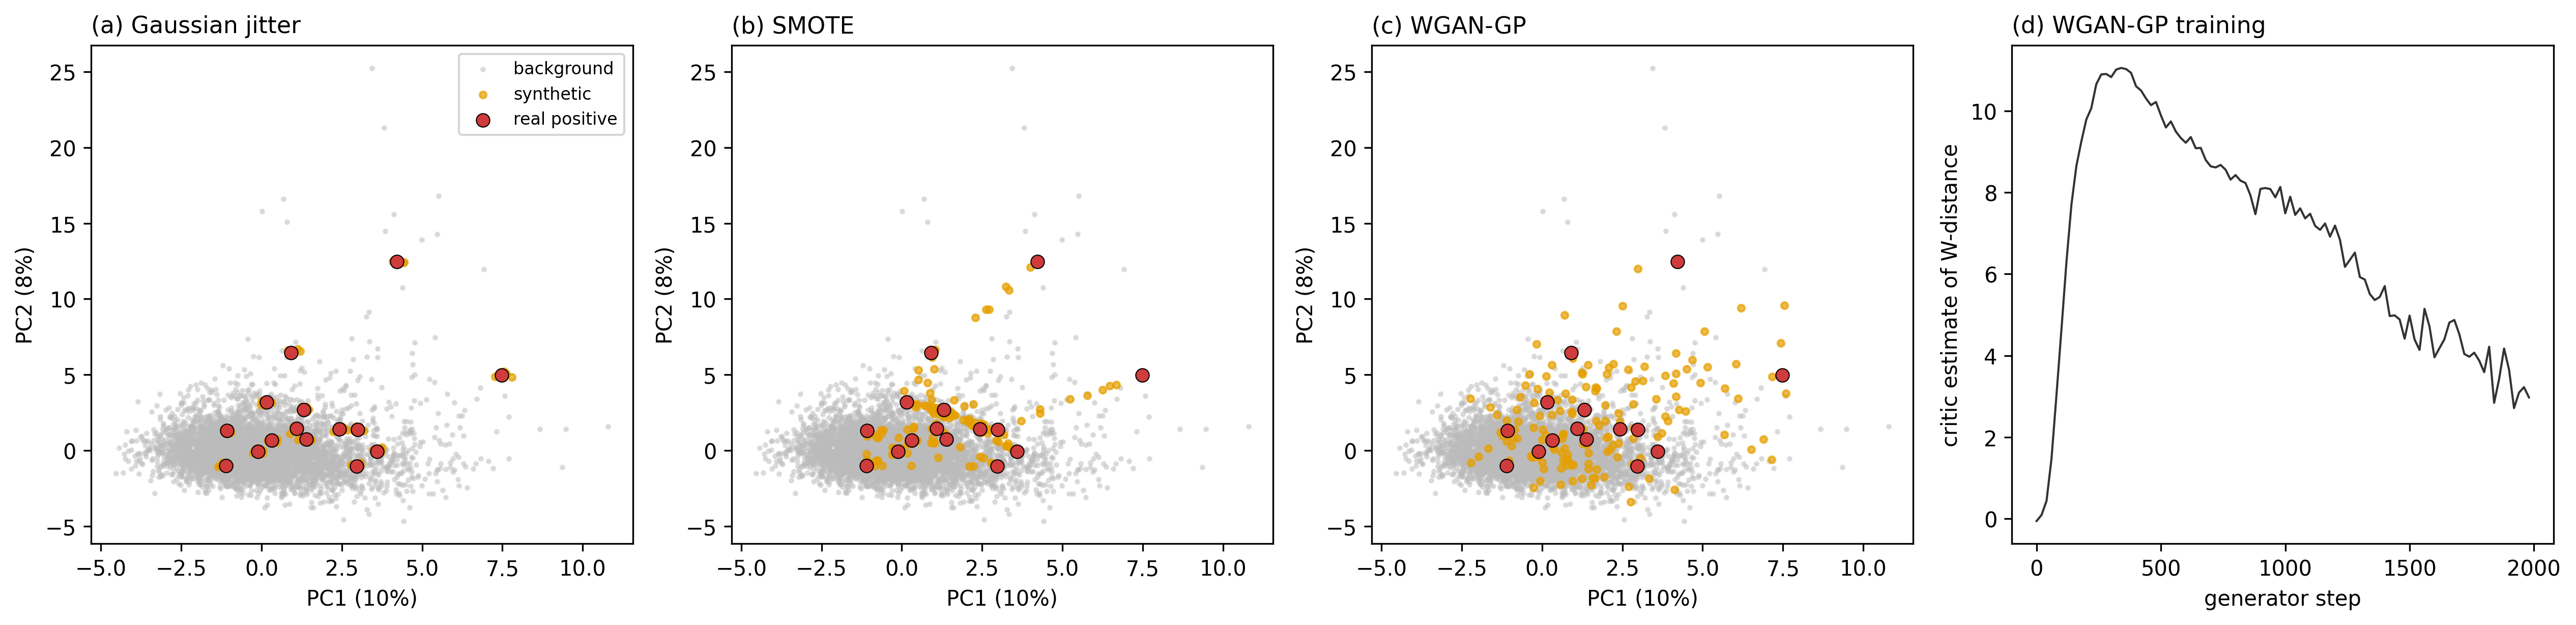
\includegraphics[width=\textwidth]{figures/fig_augmentation_superior.png}
\caption{(a--c) Synthetic positives from each generator (fitted to all 15 Superior positives) in the first two principal components of background and real positives. (d) WGAN-GP critic estimate of the Wasserstein distance during training.}\label{fig:aug-pca}
\end{figure}

\begin{figure}[t]
\centering
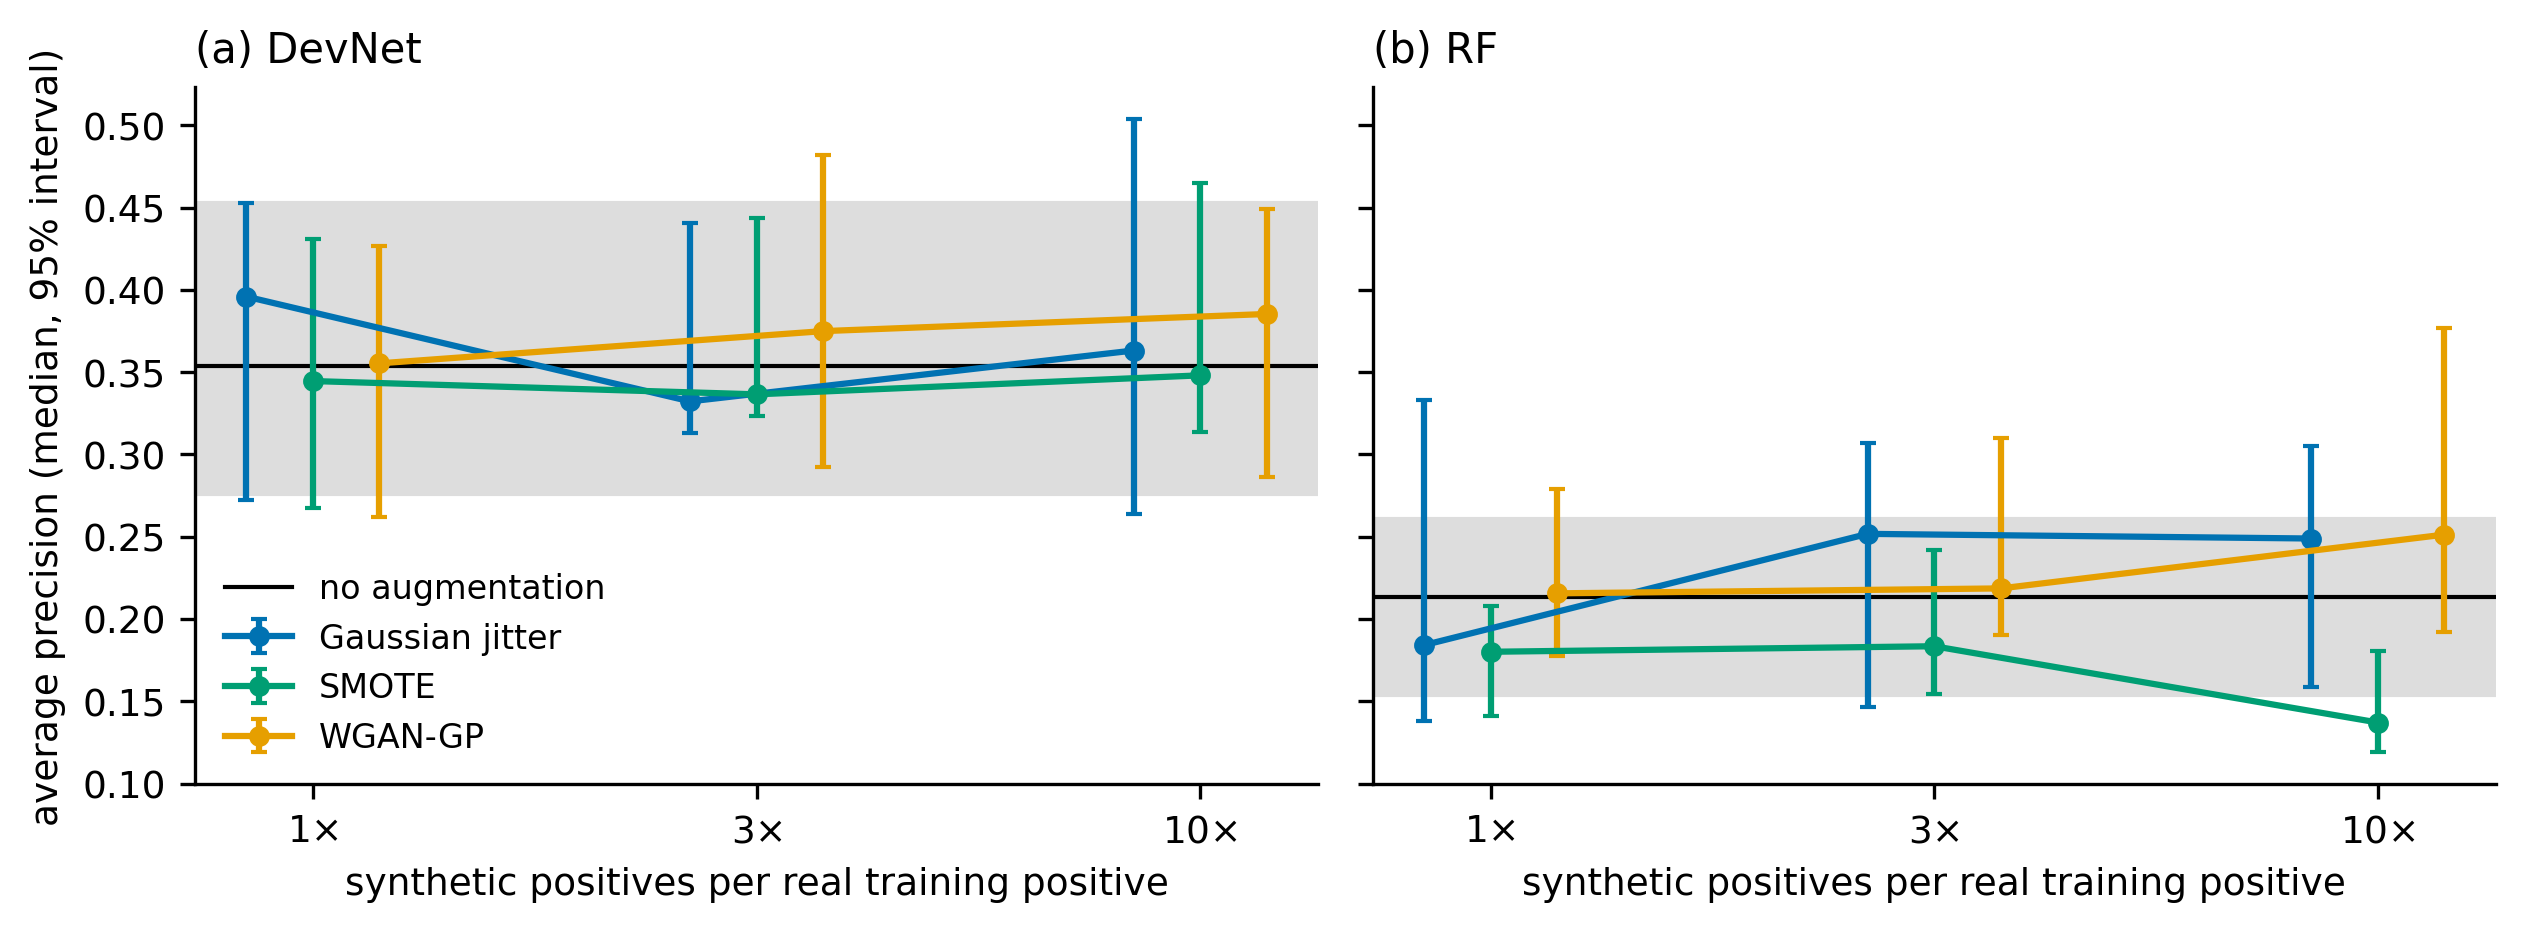
\includegraphics[width=\textwidth]{figures/fig_augmentation_performance_rev.png}
\caption{Superior average precision with fold-safe synthetic positives, by generator and number of synthetic positives per real training positive. Line and grey band: no augmentation (median and 95\% interval).}\label{fig:aug-perf}
\end{figure}

\begin{table}[t]
\caption{Effect of fold-safe positive augmentation on held-out performance, Superior (random cross-validation, identical folds; held-out positives always real). $\Delta$AP: paired difference from no augmentation in each of the six repeats (median [min, max]); wins: repeats with higher AP than without augmentation.}\label{tab:augmentation}
\scriptsize
\setlength{\tabcolsep}{2.5pt}
\begin{tabular*}{\textwidth}{@{\extracolsep\fill}lllcccc}
\toprule
Model & Generator & $m$ & AUC & AP & $\Delta$AP per repeat & wins \\
\midrule
\multirow{10}{*}{DevNet} & none & -- & 0.951 & 0.354 [0.276, 0.453] & -- & -- \\
 & Gaussian jitter & 1$\times$ & 0.952 & 0.396 [0.272, 0.453] & +0.008 [-0.005, +0.076] & 4/6 \\
 & Gaussian jitter & 3$\times$ & 0.951 & 0.332 [0.313, 0.441] & -0.008 [-0.030, +0.044] & 2/6 \\
 & Gaussian jitter & 10$\times$ & 0.950 & 0.363 [0.264, 0.504] & +0.007 [-0.016, +0.088] & 3/6 \\
 & SMOTE & 1$\times$ & 0.951 & 0.345 [0.267, 0.431] & -0.016 [-0.062, +0.067] & 2/6 \\
 & SMOTE & 3$\times$ & 0.947 & 0.337 [0.323, 0.444] & +0.005 [-0.085, +0.062] & 3/6 \\
 & SMOTE & 10$\times$ & 0.947 & 0.348 [0.313, 0.465] & +0.025 [-0.073, +0.042] & 4/6 \\
 & WGAN-GP & 1$\times$ & 0.940 & 0.355 [0.262, 0.426] & -0.003 [-0.100, +0.069] & 3/6 \\
 & WGAN-GP & 3$\times$ & 0.942 & 0.375 [0.292, 0.482] & +0.040 [-0.089, +0.077] & 4/6 \\
 & WGAN-GP & 10$\times$ & 0.943 & 0.385 [0.286, 0.449] & +0.011 [-0.035, +0.060] & 4/6 \\
\midrule
\multirow{10}{*}{RF} & none & -- & 0.973 & 0.214 [0.154, 0.261] & -- & -- \\
 & Gaussian jitter & 1$\times$ & 0.943 & 0.184 [0.138, 0.333] & -0.032 [-0.071, +0.183] & 1/6 \\
 & Gaussian jitter & 3$\times$ & 0.970 & 0.252 [0.146, 0.307] & +0.014 [-0.014, +0.110] & 4/6 \\
 & Gaussian jitter & 10$\times$ & 0.962 & 0.249 [0.159, 0.305] & +0.025 [-0.063, +0.139] & 5/6 \\
 & SMOTE & 1$\times$ & 0.958 & 0.180 [0.141, 0.208] & -0.025 [-0.094, +0.026] & 2/6 \\
 & SMOTE & 3$\times$ & 0.975 & 0.183 [0.154, 0.242] & -0.015 [-0.083, +0.075] & 3/6 \\
 & SMOTE & 10$\times$ & 0.966 & 0.137 [0.119, 0.180] & -0.050 [-0.125, -0.020] & 0/6 \\
 & WGAN-GP & 1$\times$ & 0.971 & 0.216 [0.177, 0.279] & +0.040 [-0.075, +0.065] & 4/6 \\
 & WGAN-GP & 3$\times$ & 0.973 & 0.219 [0.190, 0.310] & +0.008 [-0.046, +0.149] & 3/6 \\
 & WGAN-GP & 10$\times$ & 0.975 & 0.251 [0.192, 0.377] & +0.041 [-0.057, +0.222] & 5/6 \\
\botrule
\end{tabular*}
\end{table}

\begin{table}[t]
\caption{What the generators produce (fitted to all 15 Superior positives; 150 samples each). NN ratio: distance to the nearest real positive divided by the median nearest-neighbour distance among real positives (0 = copy). Nearest labelled neighbour: share of samples whose nearest point among positives and training background is a positive. DevNet percentile: median score percentile among the training background under the production DevNet.}\label{tab:aug-diag}
\footnotesize
\setlength{\tabcolsep}{2.5pt}
\begin{tabular*}{\textwidth}{@{\extracolsep\fill}lcccc}
\toprule
Source & NN ratio, median & NN ratio, P10 & NN is positive & DevNet pct. \\
\midrule
Real occurrences (leave-one-out) & 1.00 & 0.55 & -- & 0.997 \\
Gaussian jitter & 0.11 & 0.09 & 100\% & 0.985 \\
SMOTE & 0.26 & 0.06 & 96\% & 0.985 \\
WGAN-GP & 0.86 & 0.60 & 55\% & 0.983 \\
Background (300 random points) & 1.25 & -- & -- & 0.500 \\
\botrule
\end{tabular*}
\end{table}

\subsection{Validation-protocol audit}\label{sec:res-audit}

Rebuilding the S2 parent--child augmentation and child-level random splitting of \citet{Parsa2024} on our data gives a test AUC of 0.998--1.000 in all three provinces and for both negative-sampling rules, with 2.5--97.5 percentile ranges no wider than 0.98--1.00 (Table~\ref{tab:audit}; Fig.~\ref{fig:audit}). In 97--99\% of the test positives, at least one sibling child cell of the same occurrence is in the training set. In feature space, siblings are closer to each other (median standardised distance 2.1--3.7) than occurrences are to their nearest other occurrence (4.1--6.7) and than background points are to their nearest background neighbour (4.5--4.7; Table~\ref{tab:audit-sim}), because the coarse deep-architecture layers take identical values in sibling cells and the fine-scale layers nearly so.

The honest reference within this balanced 70/30 design is one label per occurrence with random negatives. It gives a mean AUC of 0.946 in Superior, 0.772 in Cordillera and 0.624 in Grenville, each with a very wide range over the 50 splits (0.65--1.00, 0.58--0.92 and 0.26--0.99). The child-level split therefore inflates test AUC by about 0.05, 0.23 and 0.37 respectively, the inflation being largest where real skill is lowest, and it collapses the apparent uncertainty to almost nothing. Drawing negatives from the least similar 5\% of the ground inflates AUC independently of the split: without augmentation, cosine-dissimilar negatives raise mean AUC from 0.946 to 0.990 in Superior, from 0.772 to 0.993 in Cordillera and from 0.624 to 0.833 in Grenville. Keeping all children of one parent on the same side of the split removes most, but not all, of the augmentation effect (Superior 0.957, Cordillera 0.963, Grenville 0.829 with random negatives); the remainder reflects the fourfold larger training set and spatial dependence between neighbouring occurrences in different parent cells, which only spatial blocking removes.

\begin{figure}[t]
\centering
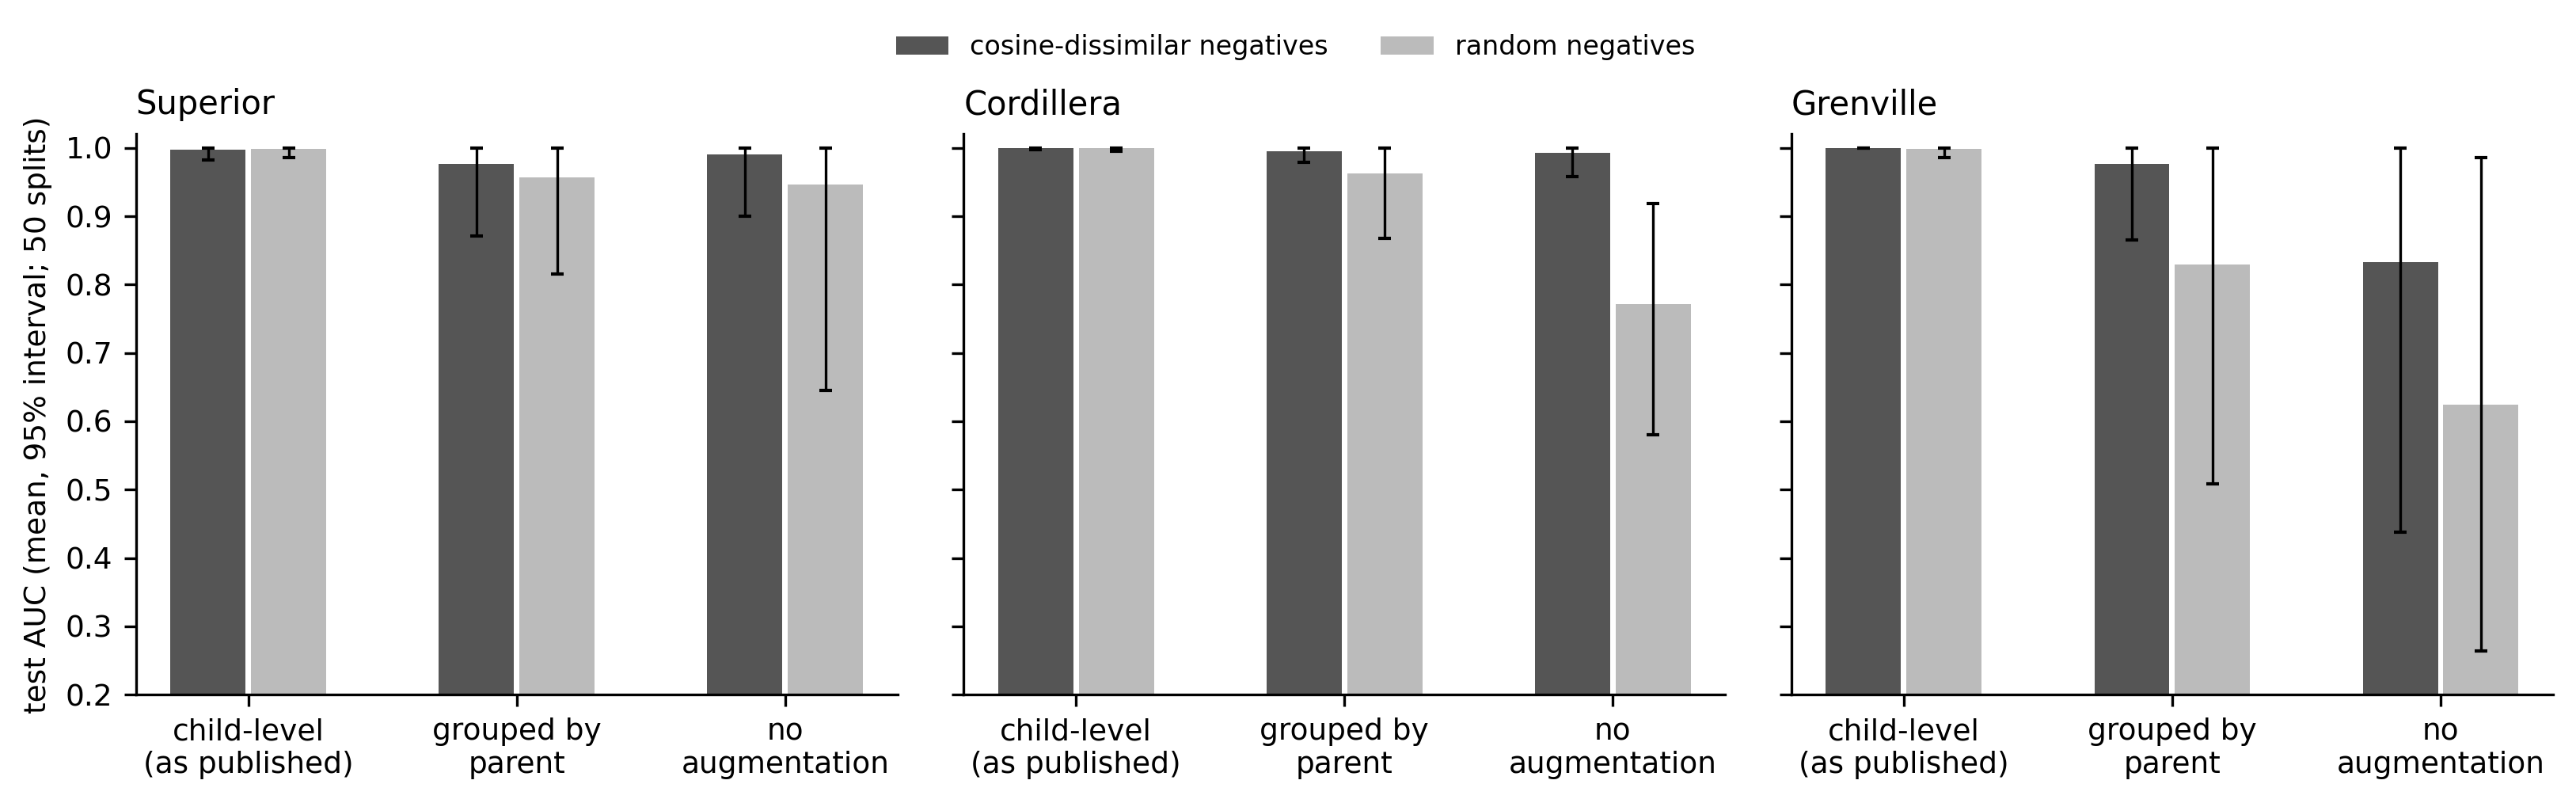
\includegraphics[width=\textwidth]{figures/fig_protocol_audit.png}
\caption{Protocol audit: random forest test AUC under S2 parent--child augmentation for three split designs and two negative-sampling rules (mean and range over 50 balanced 70/30 splits).}\label{fig:audit}
\end{figure}

\begin{table}[t]
\caption{Feature-space distance (median, standardised features) between sibling child cells of the same occurrence, from each occurrence to its nearest other occurrence, and from background points to their nearest background neighbour.}\label{tab:audit-sim}
\footnotesize
\begin{tabular*}{0.8\textwidth}{@{\extracolsep\fill}lccc}
\toprule
Region & Siblings & Nearest other occurrence & Nearest background neighbour \\
\midrule
Superior & 3.43 & 5.42 & 4.45 \\
Cordillera & 2.11 & 4.06 & 4.50 \\
Grenville & 3.69 & 6.74 & 4.66 \\
\botrule
\end{tabular*}
\end{table}

\begin{table}[t]
\caption{Protocol audit: random forest test AUC (mean and 2.5--97.5 percentile range over 50 stratified 70/30 splits of balanced labels) under the S2 parent--child augmentation of \citet{Parsa2024}, for two negative-sampling rules (cosine-dissimilar or random) and three split designs (child-level random, as published; children grouped by parent; no augmentation). Pos.: positive labels. Sibling: share of test positives with a sibling child cell in the training set.}\label{tab:audit}
\scriptsize
\setlength{\tabcolsep}{2.5pt}
\begin{tabular*}{\textwidth}{@{\extracolsep\fill}lllccc}
\toprule
Region & Negatives & Split & Pos. & Test AUC & Sibling \\
\midrule
\multirow{6}{*}{Superior} & cosine & child-level & 60 & 0.998 [0.982, 1.000] & 98\% \\
 & cosine & parent-grouped & 60 & 0.977 [0.871, 1.000] & -- \\
 & cosine & no augm. & 15 & 0.990 [0.900, 1.000] & -- \\
 & random & child-level & 60 & 0.998 [0.986, 1.000] & 98\% \\
 & random & parent-grouped & 60 & 0.957 [0.816, 1.000] & -- \\
 & random & no augm. & 15 & 0.946 [0.645, 1.000] & -- \\
\midrule
\multirow{6}{*}{Cordillera} & cosine & child-level & 108 & 1.000 [0.997, 1.000] & 97\% \\
 & cosine & parent-grouped & 108 & 0.995 [0.979, 1.000] & -- \\
 & cosine & no augm. & 27 & 0.993 [0.958, 1.000] & -- \\
 & random & child-level & 108 & 1.000 [0.995, 1.000] & 97\% \\
 & random & parent-grouped & 108 & 0.963 [0.868, 1.000] & -- \\
 & random & no augm. & 27 & 0.772 [0.580, 0.918] & -- \\
\midrule
\multirow{6}{*}{Grenville} & cosine & child-level & 48 & 1.000 [1.000, 1.000] & 99\% \\
 & cosine & parent-grouped & 48 & 0.976 [0.865, 1.000] & -- \\
 & cosine & no augm. & 12 & 0.833 [0.438, 1.000] & -- \\
 & random & child-level & 48 & 0.998 [0.986, 1.000] & 99\% \\
 & random & parent-grouped & 48 & 0.829 [0.508, 1.000] & -- \\
 & random & no augm. & 12 & 0.624 [0.264, 0.986] & -- \\
\botrule
\end{tabular*}
\end{table}

\subsection{Model interpretation}\label{sec:res-shap}

With the rank-based direction rule, RF and DevNet agree on the sign of the effect for all ten of their jointly most important features in each province (Table~\ref{tab:shap}; Appendix~\ref{app:shap}). Read from the sign of the mean SHAP value instead, the two models would appear to disagree on most of these features, an artefact of the two explainers' different baselines (Section~\ref{sec:shap}). The importance rankings of RF and DevNet are moderately correlated ($\rho_{\mathrm{S}} = 0.40$--$0.56$ across all pruned features).

In Superior (Fig.~\ref{fig:shap}) DevNet ranks LAB depth first, followed by Bouguer GLCM correlation, the 100~km high-pass Bouguer anomaly, deep magnetic-worm proximity and Moho depth; RF ranks the horizontal-gradient magnitude of deep-source magnetics first, then LAB depth and fault proximity. Both models score ground as more prospective where the LAB and Moho are shallower, where the long-wavelength residual gravity is positive, near faults and deep gravity worms, over magnetic highs (DRTP 1VD) and where the magnetic texture is rougher (TMI GLCM contrast), and as less prospective close to deep magnetic worms and where deep-source magnetic gradients are high. DevNet additionally gives large positive attributions to the few explained points mapped as alkaline-favourable lithology, and to points outside Archean terrane. In Cordillera both models treat Mesozoic terranes as unfavourable and Proterozoic terranes as favourable, and both rate fault and passive-margin proximity positively. In Grenville both rank deep-source magnetics, magnetic tilt and gravity texture highest, but given the weak predictive skill there these attributions describe the signal the models attempted to use rather than a reliable control.

\begin{figure}[t]
\centering
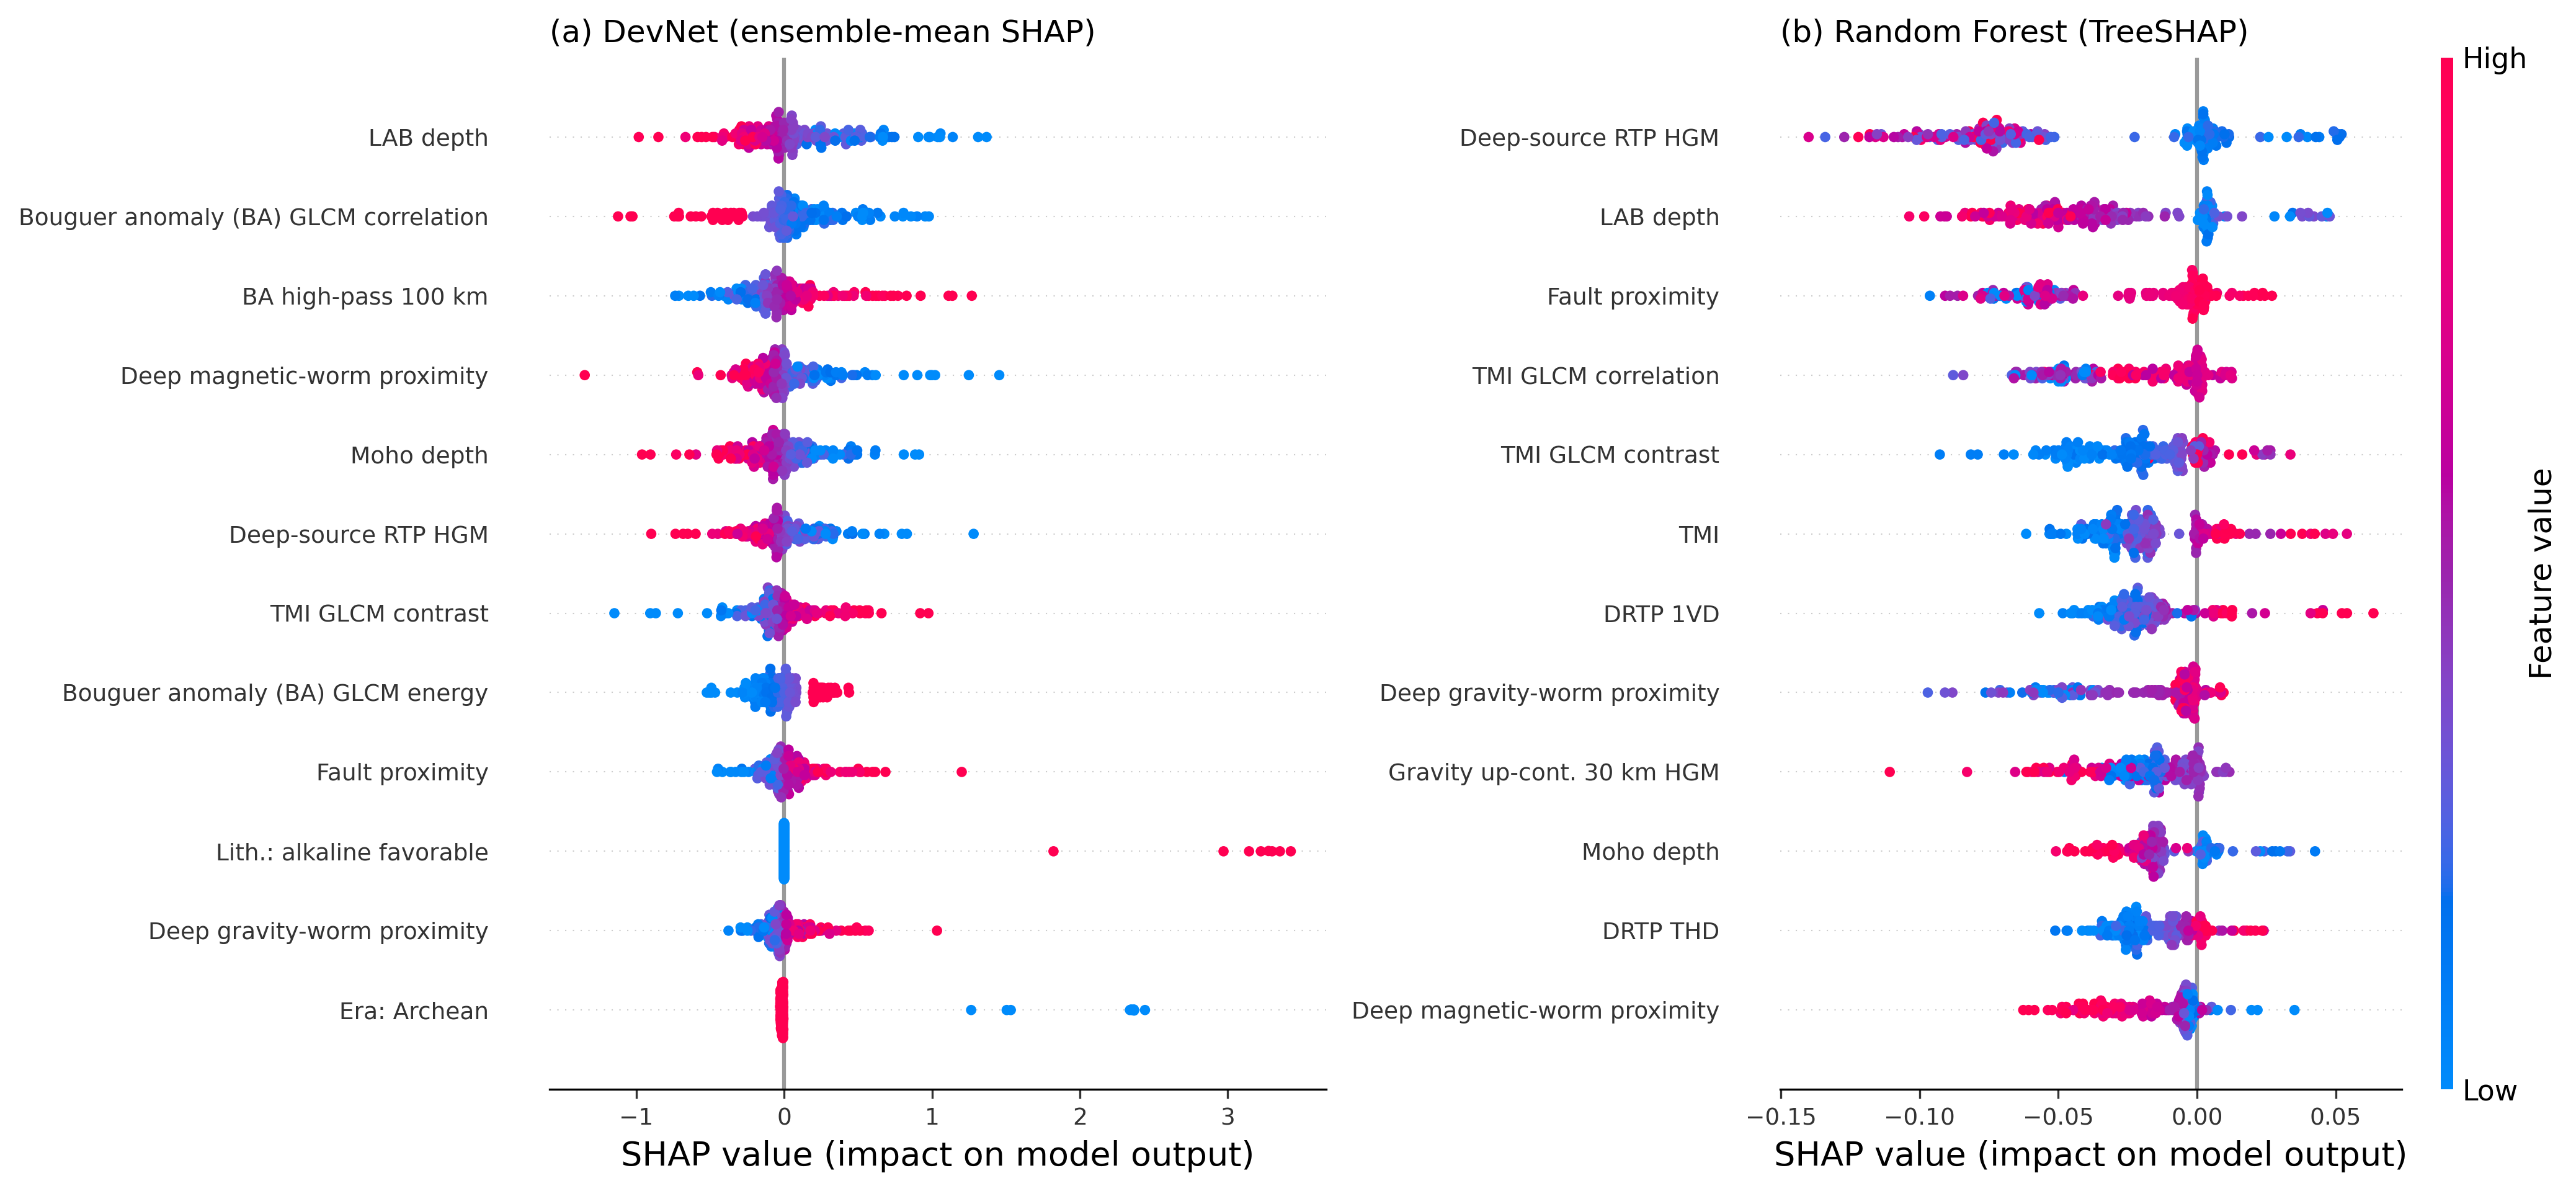
\includegraphics[width=\textwidth]{figures/fig_shap_superior_rev.png}
\caption{SHAP summaries for Superior: (a) DevNet (DeepSHAP on its quantile-transformed inputs, mean over the five ensemble members) and (b) RF (TreeSHAP). Each point is one explained sample; colour is the feature value. SHAP magnitudes are not comparable between models (unbounded anomaly score vs probability).}\label{fig:shap}
\end{figure}

\begin{table}[t]
\caption{Superior: the ten jointly most important features (mean $|$SHAP$|$, normalised per model). Rank among 35 features; direction $\uparrow$/$\downarrow$: higher values (or presence) raise/lower the score, with Spearman $\rho$ between feature value and SHAP value.}\label{tab:shap}
\scriptsize
\setlength{\tabcolsep}{2.5pt}
\begin{tabular*}{\textwidth}{@{\extracolsep\fill}lcccc}
\toprule
Feature & DevNet rank & DevNet dir. & RF rank & RF dir. \\
\midrule
LAB depth & 1 & $\downarrow$ (-0.97) & 2 & $\downarrow$ (-0.89) \\
Deep-source RTP HGM & 6 & $\downarrow$ (-0.96) & 1 & $\downarrow$ (-0.74) \\
Bouguer anomaly (BA) GLCM correlation & 2 & $\downarrow$ (-0.90) & 19 & $\downarrow$ (-0.86) \\
BA high-pass 100 km & 3 & $\uparrow$ (+0.97) & 16 & $\uparrow$ (+0.81) \\
Deep magnetic-worm proximity & 4 & $\downarrow$ (-0.96) & 12 & $\downarrow$ (-0.94) \\
TMI GLCM contrast & 7 & $\uparrow$ (+0.95) & 5 & $\uparrow$ (+0.92) \\
Fault proximity & 9 & $\uparrow$ (+0.96) & 3 & $\uparrow$ (+0.89) \\
Moho depth & 5 & $\downarrow$ (-0.97) & 10 & $\downarrow$ (-0.86) \\
Deep gravity-worm proximity & 11 & $\uparrow$ (+0.94) & 8 & $\uparrow$ (+0.81) \\
DRTP 1VD & 14 & $\uparrow$ (+0.96) & 7 & $\uparrow$ (+0.86) \\
\botrule
\end{tabular*}
\end{table}

\subsection{Prospectivity maps and an external check}\label{sec:res-maps}

The production DevNet and RF maps (Fig.~\ref{fig:maps}) both concentrate the highest classes in the eastern Abitibi around the Montviel--Lac Shortt cluster and in the south-central Superior Province. DevNet spreads its high-ranked ground further along the southern margin of the province, from the Kapuskasing area to the eastern Abitibi, whereas RF concentrates it around the training occurrences. In the Kapuskasing area (Fig.~\ref{fig:ksz}) DevNet's top 1\% and 5\% classes form a coherent, north-north-east trending band that follows the mapped trace of the KSZ and its alkaline complexes, extending well beyond the two training occurrences located there. As a blind test we scored Clay-Howells, a drill-tested Fe--REE--Nb prospect with reported resources on the KSZ \citep{OGS2011} that is not among the training labels and lies 79~km from the nearest one. At its recorded location both models place it among the top 2\% of the 8,000 random background points of the province: DevNet at the 98.5th percentile and RF at the 99.4th, the latter with a probability of only 0.04 while 86\% of the background receives exactly zero.

\begin{figure}[t]
\centering
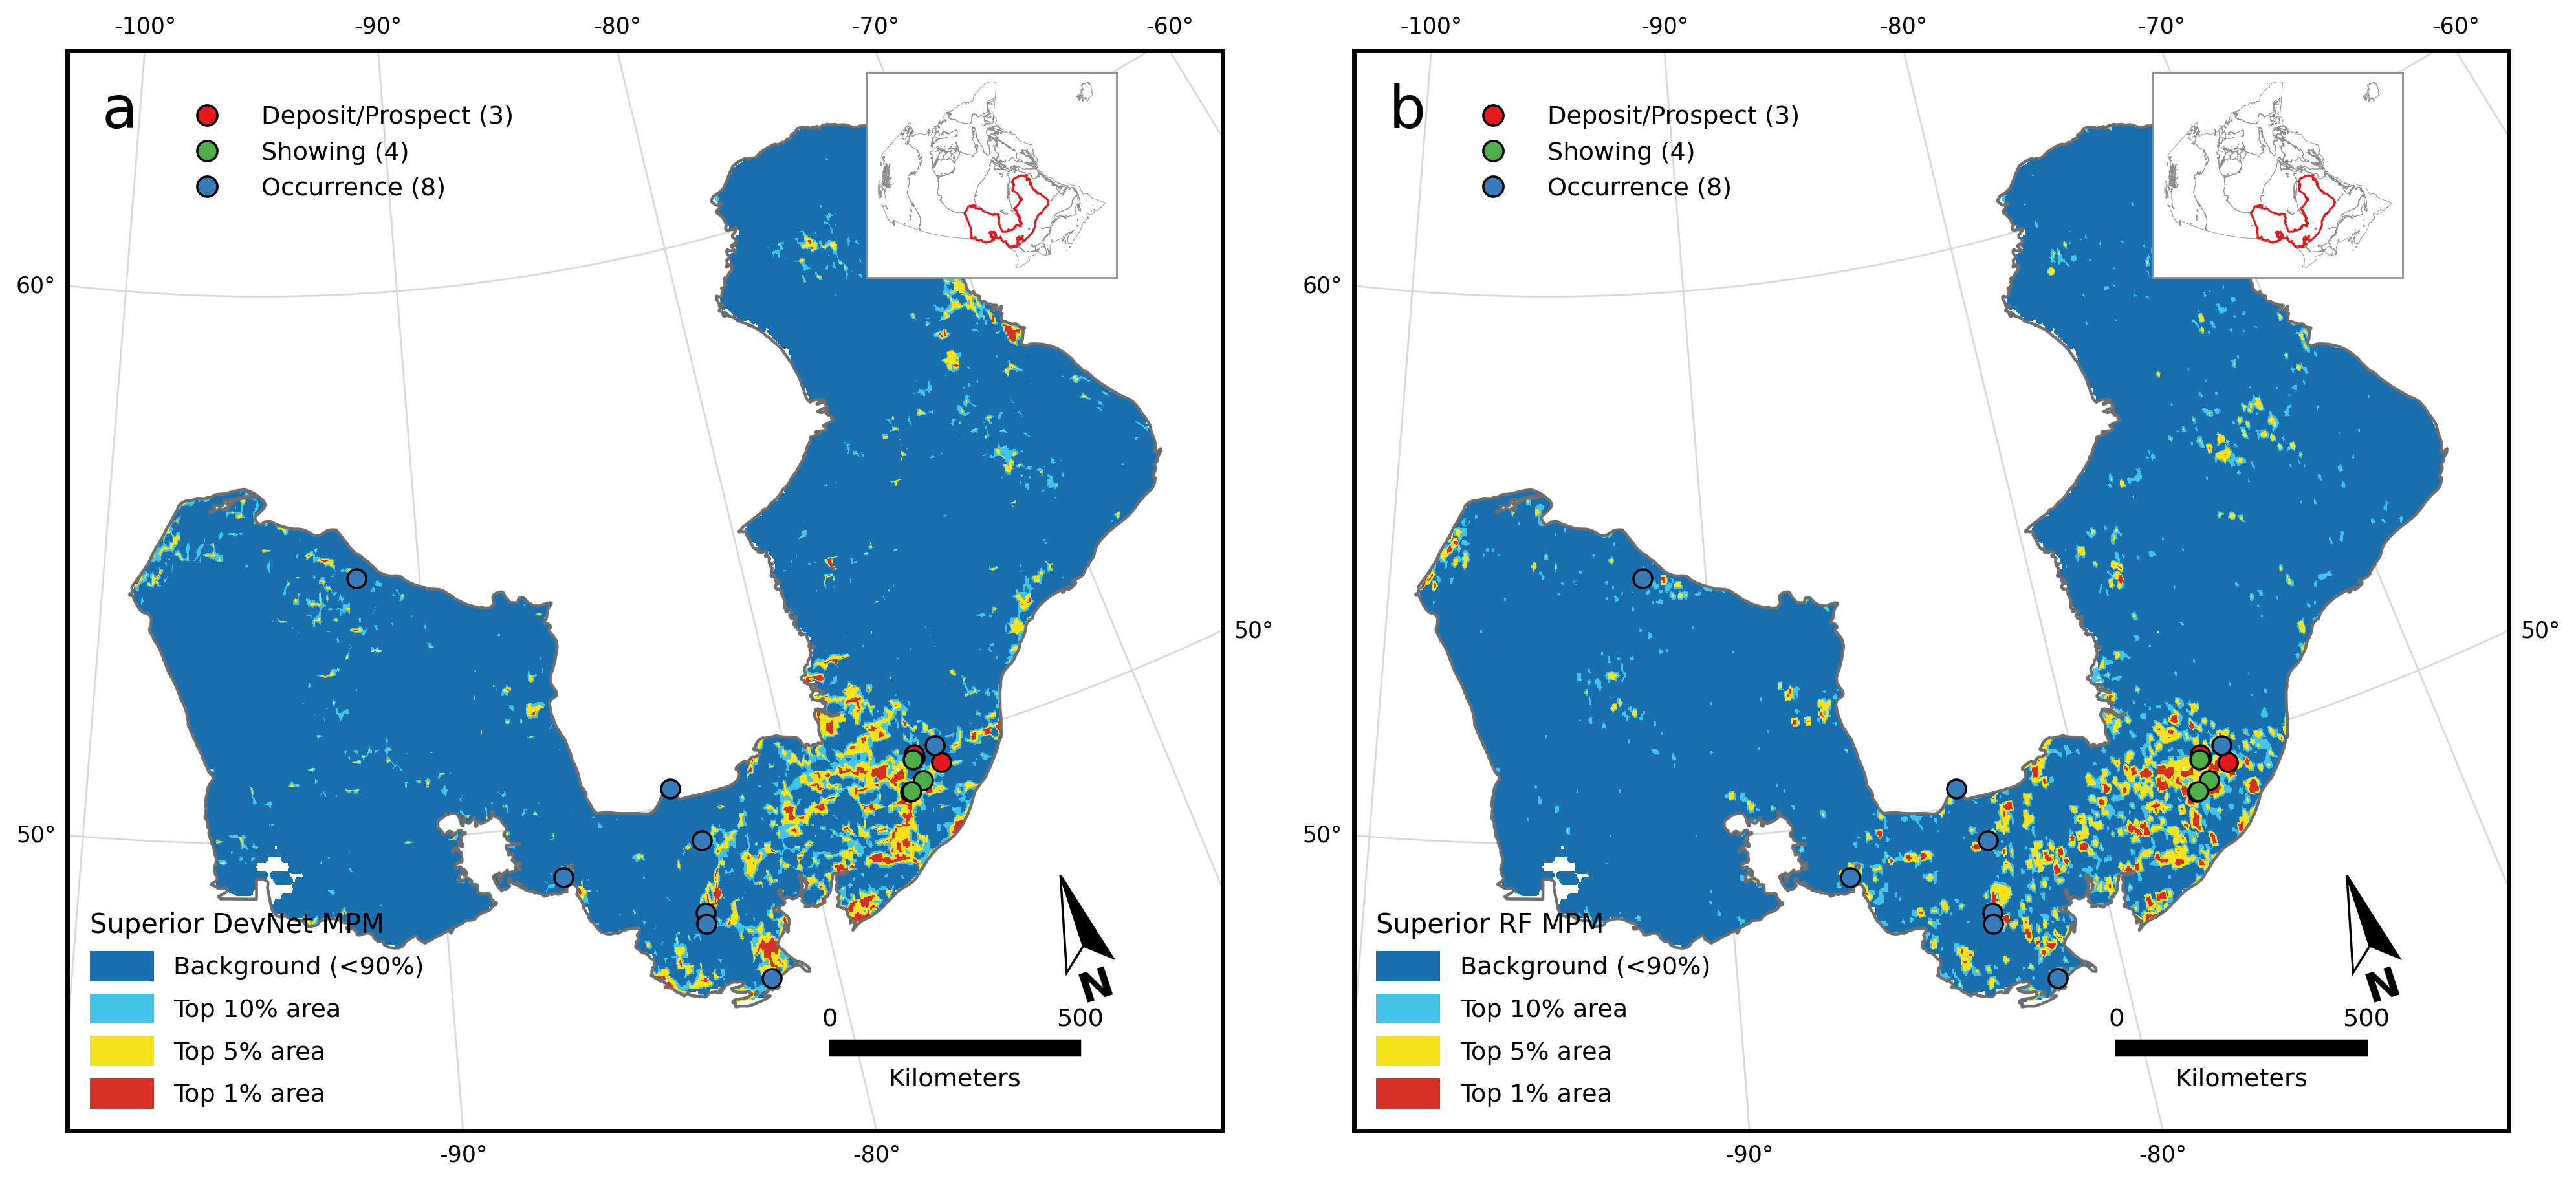
\includegraphics[width=\textwidth]{figures/fig_map_superior_rev.png}
\caption{Superior prospectivity maps from the production (a) DevNet and (b) RF models, classified by score percentile over the mapped area (top 1\%, 5\% and 10\%), with known occurrences by development class (Canada Atlas Lambert). Scores on the 0.1$^\circ$ prediction grid were interpolated to a 2~km raster.}\label{fig:maps}
\end{figure}

\begin{figure}[t]
\centering
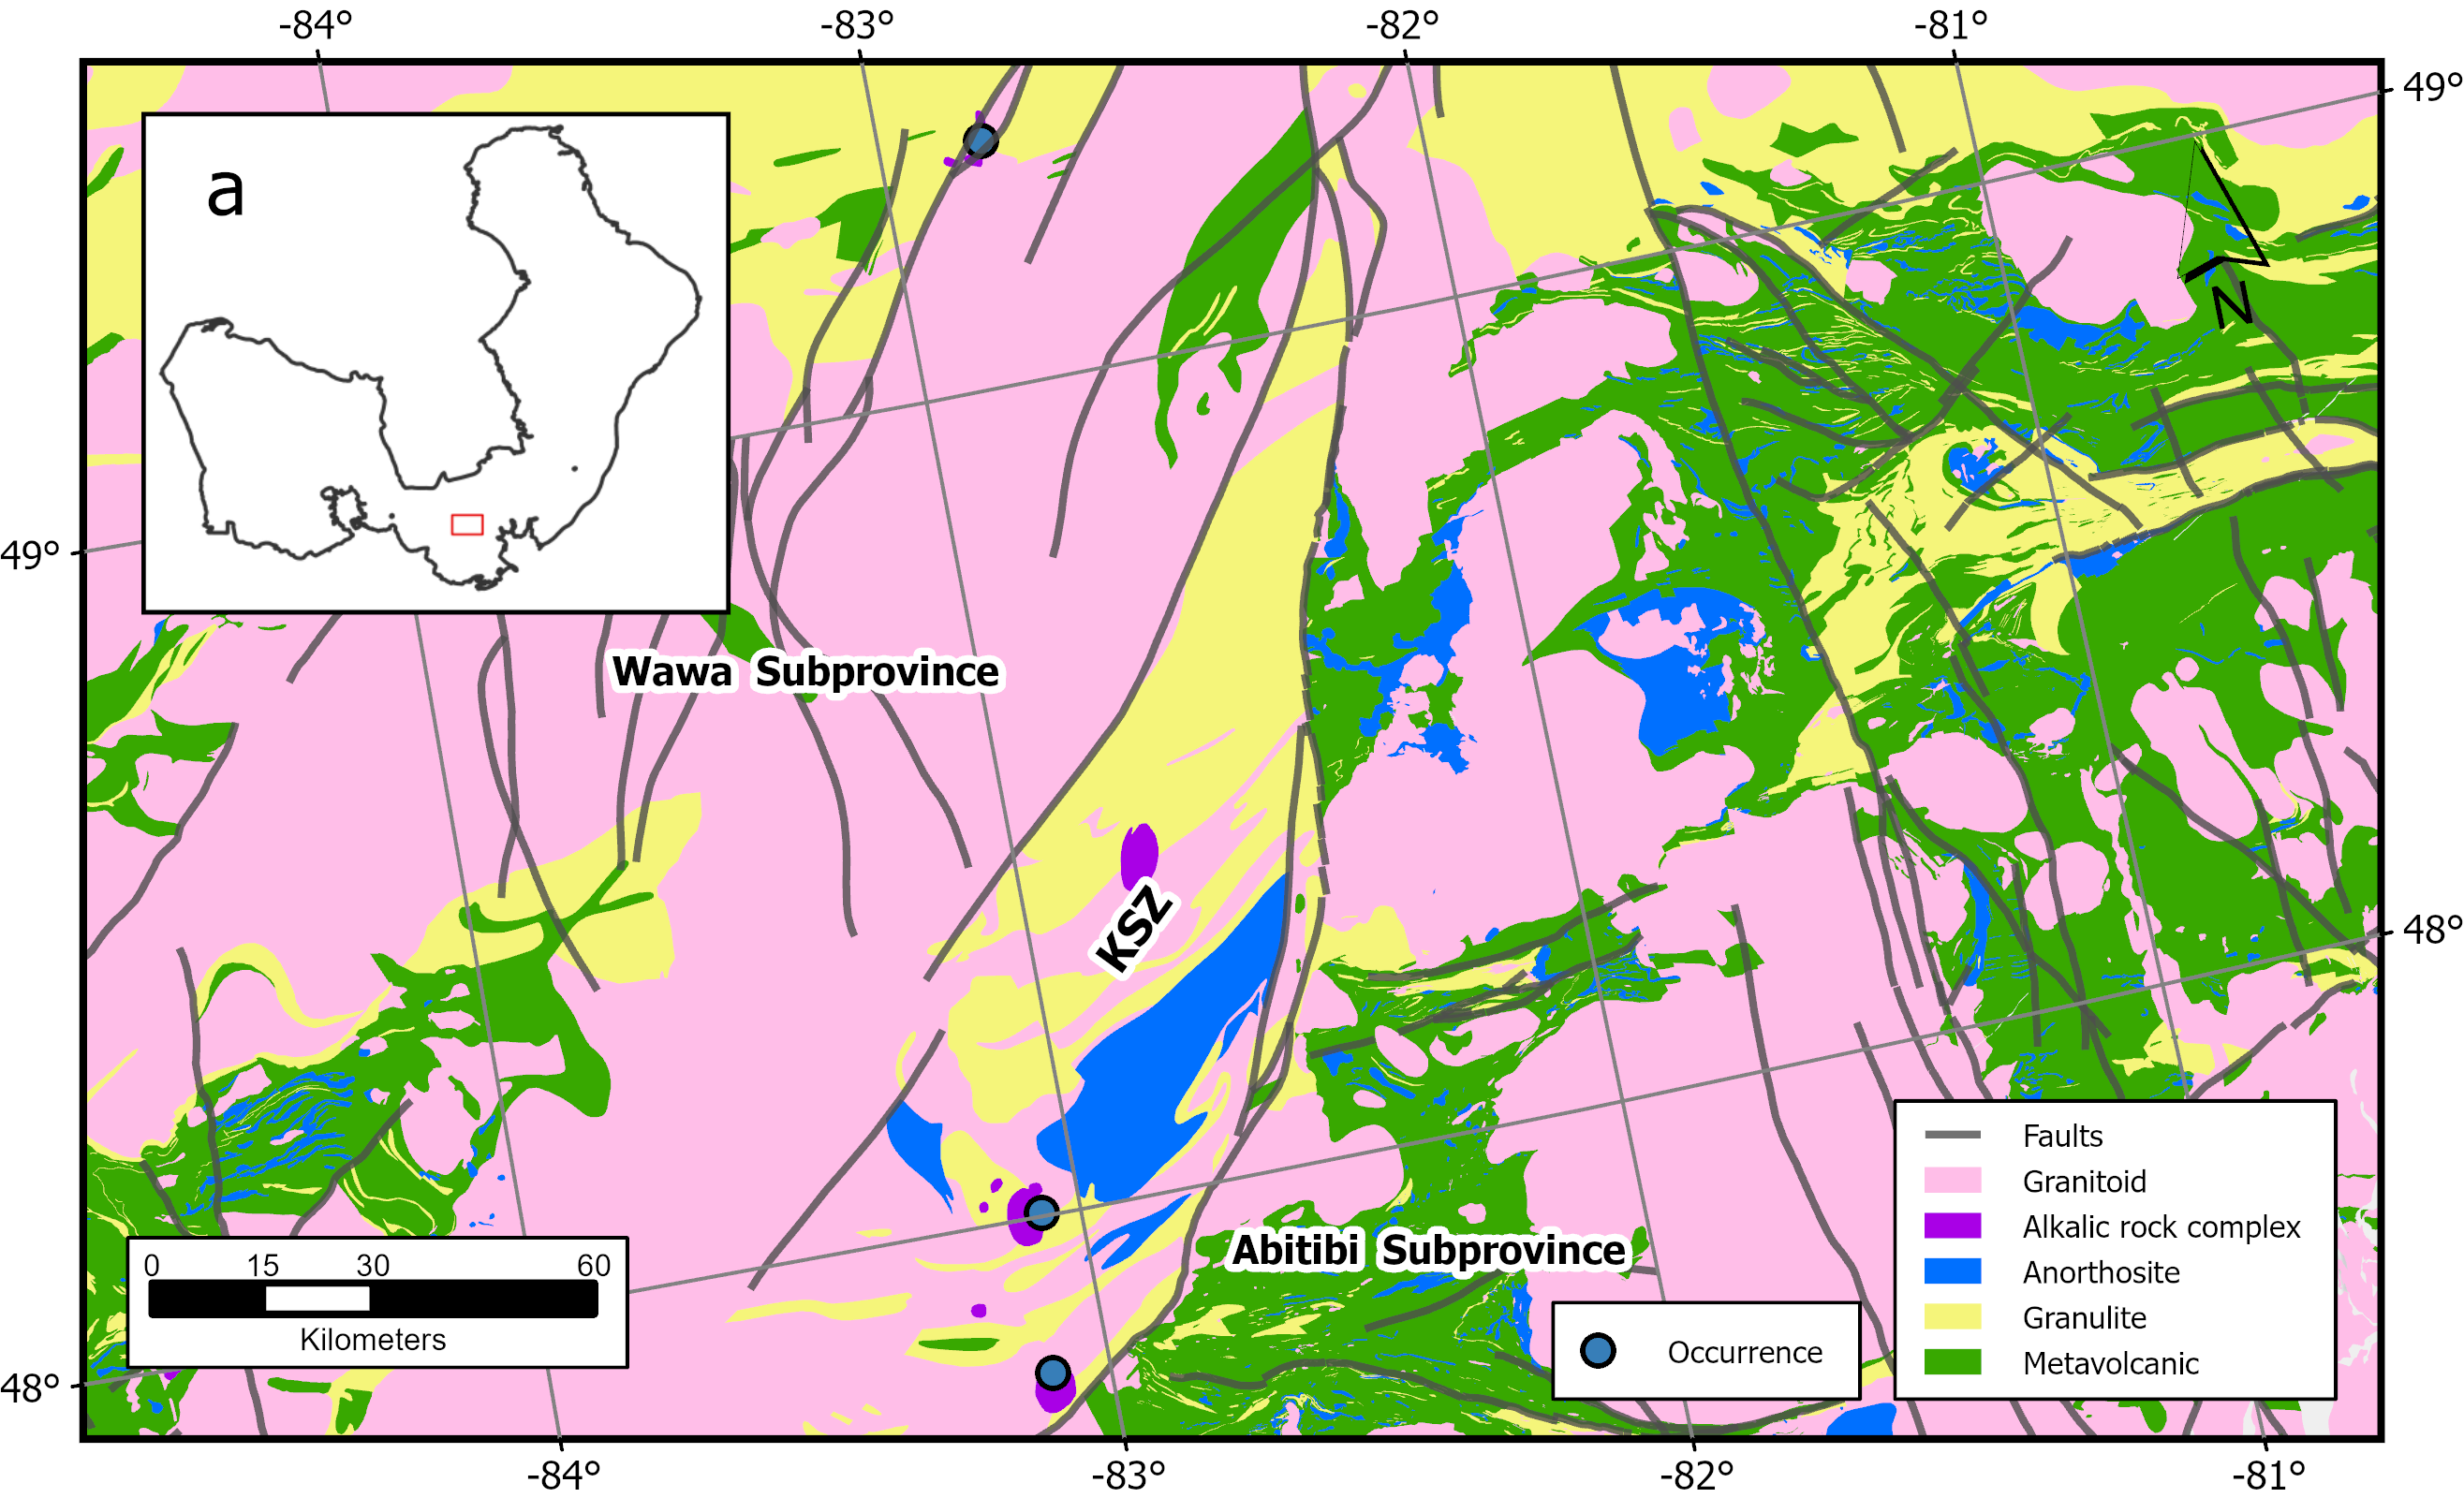
\includegraphics[width=0.49\textwidth]{figures/fig_ksz_geology.png}\hfill
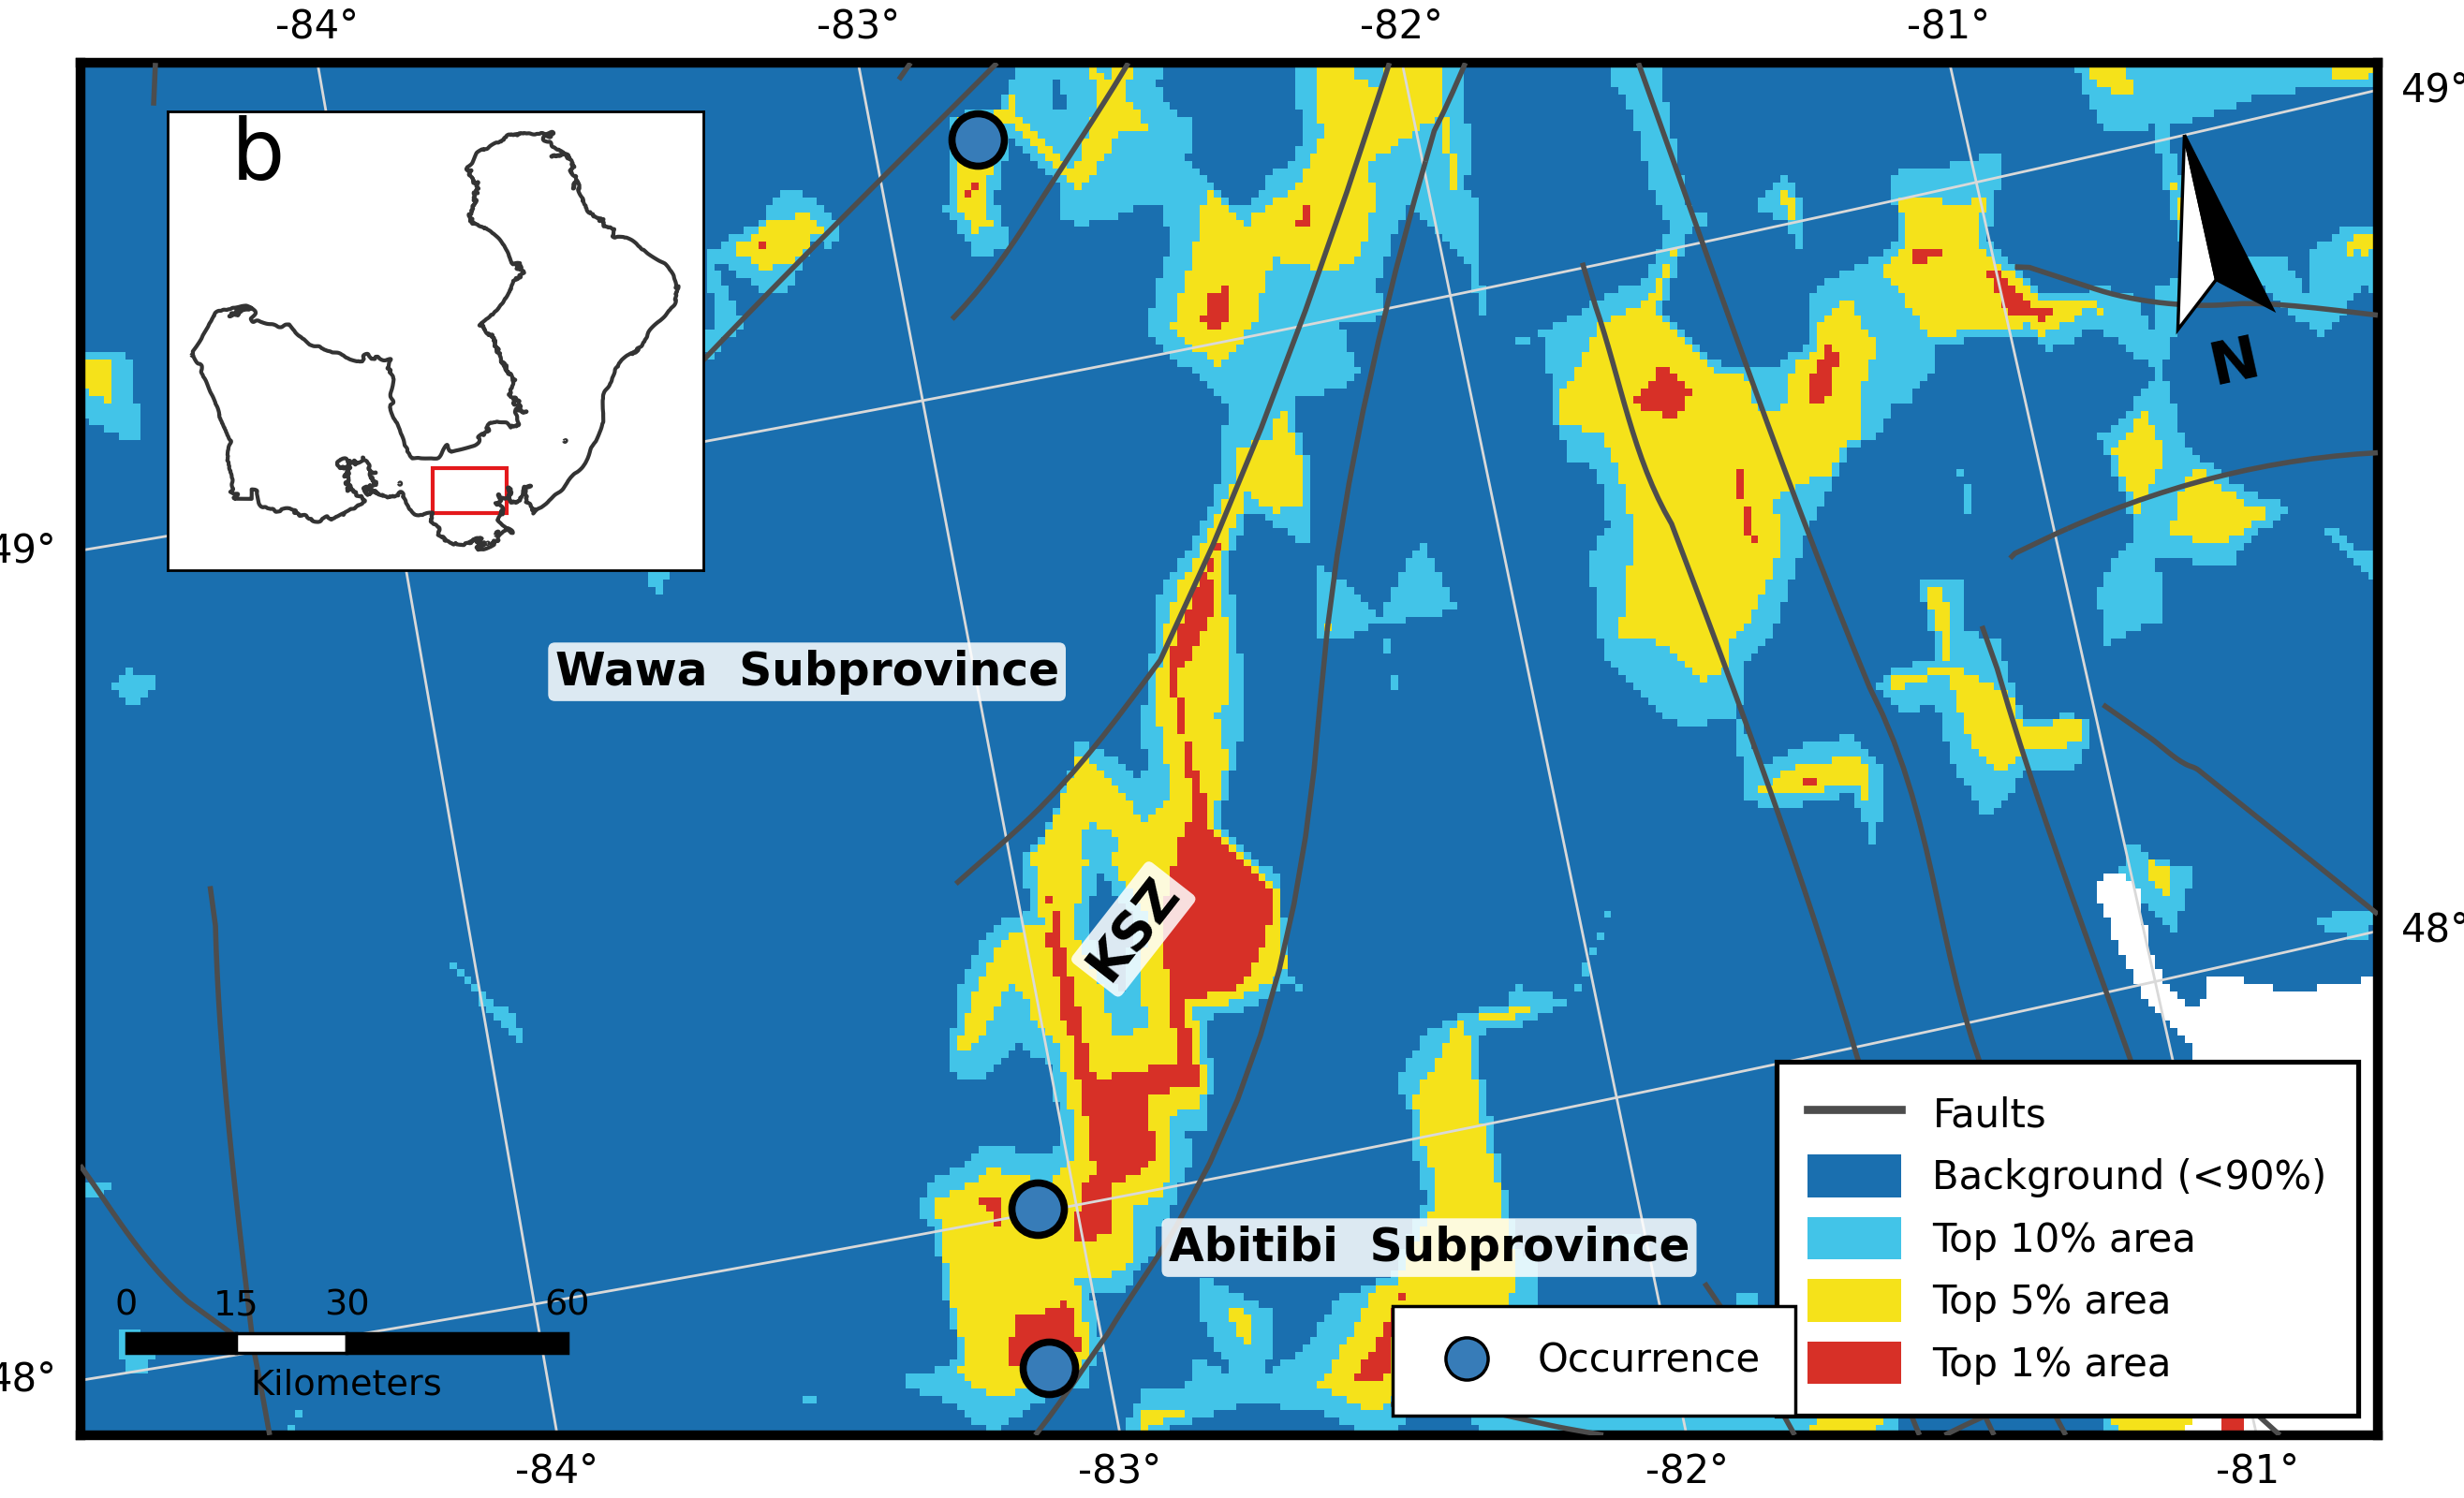
\includegraphics[width=0.49\textwidth]{figures/fig_ksz_rev.png}
\caption{External check in the Kapuskasing area. (a) Regional geology with the Kapuskasing Structural Zone (KSZ) and alkalic rock complexes \citep{Gittins1967,Percival1994}, compiled from \citet{Heather1995} and \citet{Montsion2018}. (b) DevNet top 1\%, 5\% and 10\% classes (province-wide percentiles), with faults from the compilation used as an evidence layer, on the same frame as (a).}\label{fig:ksz}
\end{figure}

The DevNet map is also more stable with respect to individual occurrences (Fig.~\ref{fig:stability}). When each of the 15 occurrences is left out in turn, 90\% of the grid nodes in the full DevNet model's top 5\% remain in the top 5\% in at least 12 of the 15 refitted models, and 2\% in fewer than half of them; for RF the shares are 55\% and 25\%. RF's top classes therefore depend strongly on which occurrences are known, whereas DevNet's follow properties shared by many of them.

\begin{figure}[t]
\centering
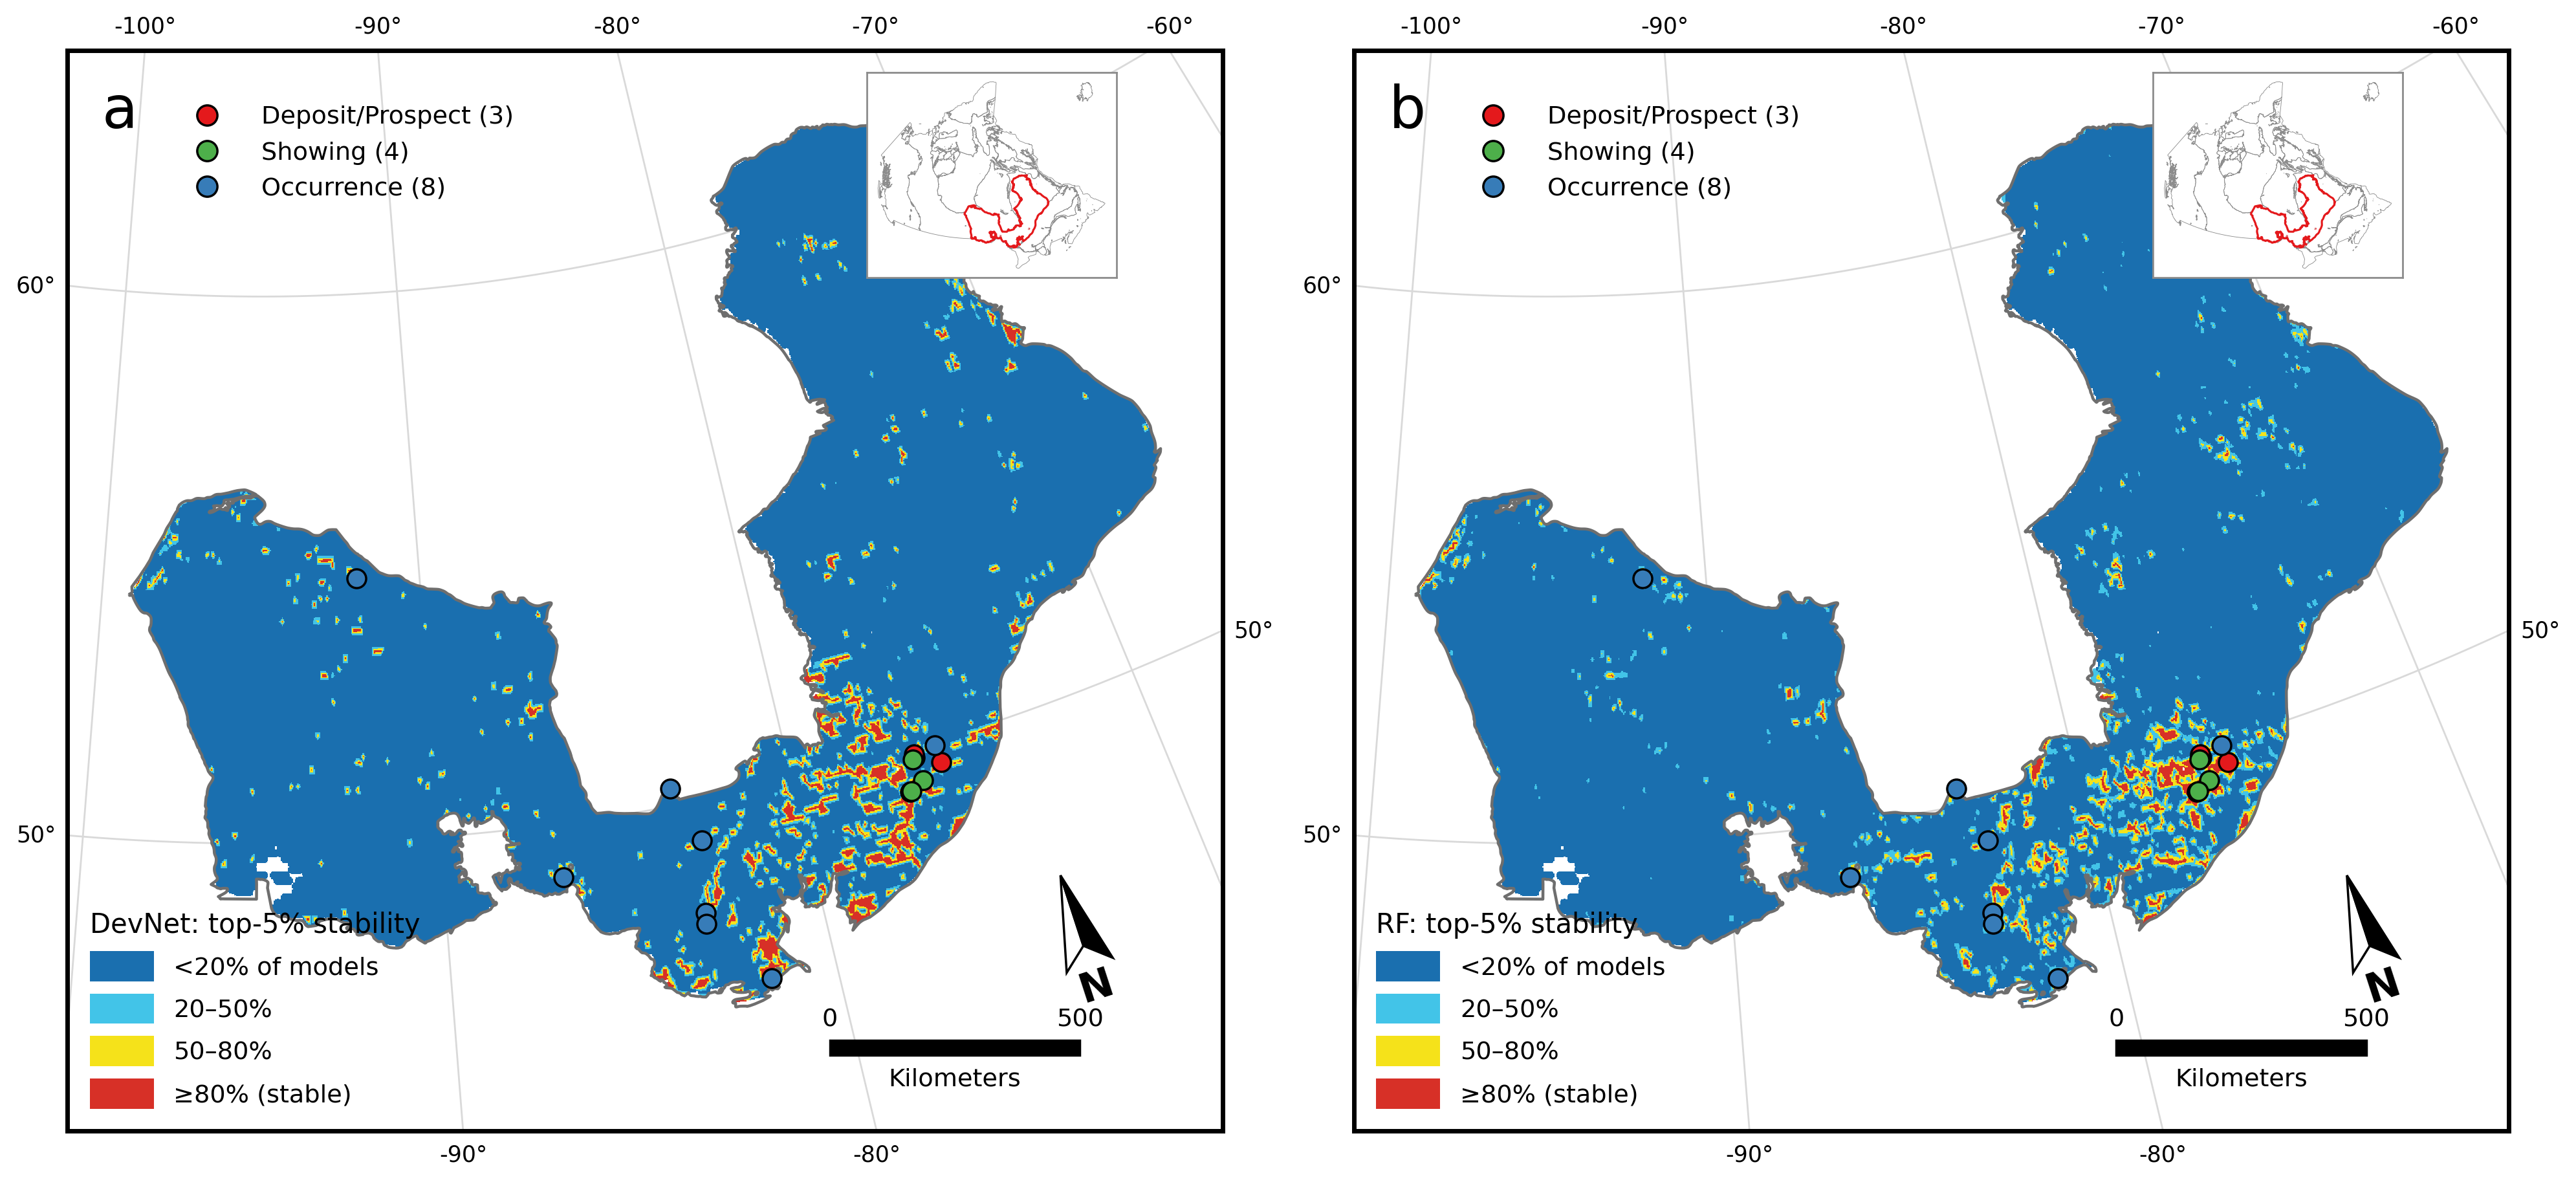
\includegraphics[width=\textwidth]{figures/fig_map_stability_rev.png}
\caption{Stability of the Superior top-5\% class with respect to individual occurrences: share of the 15 leave-one-occurrence-out models that place each 2~km cell in the province's top 5\%, for (a) DevNet and (b) RF.}\label{fig:stability}
\end{figure}

%% ===================================================================
\section{Discussion}\label{sec:discussion}

\subsection{Where semi-supervised anomaly detection helps}\label{sec:disc-devnet}

Under random cross-validation DevNet's lead in Superior is within the uncertainty of 15 positives, and it is clearly worse than the tree-based models in Cordillera and Grenville. A study that stopped there would conclude that the semi-supervised formulation offers no clear predictive advantage. The spatially blocked results show why that conclusion would be premature for Superior. RF and bagging-PU, which learn a sharp decision boundary around the training positives, lose about half of their AP once the nearest training occurrence is 100--200~km away, whereas DevNet's AP changes little. The deviation loss asks only that labelled occurrences score far above a background that is pulled towards a common reference; it does not have to carve out the neighbourhood of each training positive, and its scores vary smoothly with the deep lithospheric and potential-field controls that the occurrences share (Section~\ref{sec:res-shap}). This is the behaviour an exploration model needs, because the ground worth ranking is precisely the ground far from known occurrences. In Superior, where one tight cluster dominates the label set, a random split rewards learning that cluster; a spatial split rewards learning what the scattered occurrences have in common.

The geography-only baseline sharpens this interpretation (Section~\ref{sec:res-geography}). In Cordillera and Grenville, where the tree-based learners beat DevNet under random splits, a forest that sees only coordinates does as well or better, so DevNet's deficit there is a deficit in memorising where occurrences cluster, not in learning geology. A smooth model cannot memorise positions in this way, and for a prospectivity model that is to rank unexplored ground it should not. Like a regularised logistic regression, DevNet is outperformed precisely where location alone is predictive; where location alone is not predictive (Superior), the smooth models lead, and DevNet leads most clearly where the test requires extrapolation. A random-split comparison in a province with clustered occurrences is therefore largely a contest in spatial memorisation. The design of DevNet matters within this smooth model class (Appendix~\ref{app:sensitivity}, Table~\ref{tab:ablation}). Its score is a sum of a few ReLU ridges in the space of its inputs, so its resolution along each feature is set by how that feature is scaled; on z-scored, strongly skewed layers a handful of extreme values occupy most of the input range and the bulk of the ground is compressed into a narrow interval. Quantile-normal inputs give every feature a comparable, rank-based scale, the information that trees exploit through their thresholds, while keeping the score smooth. In the ablation this accounts for most of the gain: in Superior, quantile inputs alone raise AP from 0.209--0.272 to 0.278--0.328 across protocols, and in Grenville the random-split AP from 0.040 to 0.113. Background-heavy batches serve the premise of the deviation loss, whose inlier term is an average over the background rows of each batch: with 16 rows per step the reference behaviour of the background would be learned from about 5,000 draws in total, with 240 rows from about 72,000, while the positives are not repeated more often. They help clearly with z-scored inputs (Superior, 100~km blocks: 0.209 to 0.244) and add a smaller, less consistent gain on top of quantile inputs (a higher median AP under every protocol, but a higher AP in only two or three of six repeats). Training for longer, by contrast, repeats the dozen positives and pushes the network towards memorising their neighbourhoods: with z-scored inputs, ten times more steps raised random-split AP but lowered spatial transfer (Superior, 100~km blocks: 0.190 against 0.209), and a nested spatial early-stopping rule selected 200--300 steps in Superior. What DevNet needs is a better view of its inputs and more background per update, not more training.

The Cordilleran and Grenville results bound this conclusion. Where positives are comparatively plentiful and clustered (Cordillera), or the geophysical signal is weak (Grenville), the tree-based learners are as good or better and no model transfers well between blocks. DevNet is therefore not a universal replacement for discriminative baselines; its advantage is specific to the combination of very few positives, a shared deep control and the need to extrapolate. nnPU, which shares DevNet's network, inputs and training budget and differs only in its loss, also holds up under spatial blocking in Superior (AP 0.23--0.24), so much of the advantage over the tree-based learners belongs to smooth neural scorers in general rather than to the deviation objective alone. DevNet is nonetheless ahead of nnPU under every protocol in Superior ($\Delta$AP $+0.04$ to $+0.14$, higher in five or six of six repeats, significant only with 50~km blocks), nnPU fails in Cordillera and Grenville (AUC 0.57--0.60), and its AP depends on a class prior that is unknown in practice (0.21--0.30 for $\pi$ between 0.005 and 0.05; Table~\ref{tab:prior}).

\subsection{Why the provinces differ}\label{sec:disc-provinces}

Grenville is the weakest of the three provinces for every model and Superior the strongest. The evidence layers are the same national compilations everywhere and almost complete (about 0.01\% of values missing in each province), so the contrast does not reflect data coverage. It follows instead from the label sets and from the geology they sample (Table~\ref{tab:region-diag}).

First, the effective number of independent occurrences is smaller than the count suggests, and smallest in Grenville. Merging occurrences within 10~km leaves 12 sites of 15 occurrences in Superior, 17 of 27 in Cordillera and 8 of 12 in Grenville, and in Cordillera and Grenville more than half of the occurrences share a site with another (median distance to the nearest other occurrence 7~km, against 31~km in Superior). Under a random split such neighbours fall on both sides, which is why coordinates alone score well in these two provinces (Section~\ref{sec:res-geography}) and why their skill collapses under blocking.

Second, only in Superior do distant occurrences share a geophysical signature. There the far-neighbour index has a median of 0.005, an order of magnitude below that of random pseudo-occurrences (0.049; 5th percentile 0.022): an occurrence resembles another occurrence more than 100~km away more closely than it resembles all but a few background points. In Cordillera (0.032 against 0.027) and Grenville (0.046 against 0.066) the index falls within the range of the random sets, so there is no shared signature for a model to transfer. The univariate evidence agrees: the median feature separates occurrences from background with $|\mathrm{AUC}-0.5| = 0.15$ in Superior but only 0.05 and 0.06 in Cordillera and Grenville, where three features and one feature respectively exceed 0.25.

Third, the Grenville label set mixes carbonatites of different ages and tectonic settings. Crevier is a late-Grenvillian alkaline--carbonatite intrusion of about 957~Ma \citep{Groulier2020}. St-Honoré, with Terres Rompues on the same complex, was emplaced at about 580~Ma in the Saguenay graben of the St.~Lawrence rift system \citep{Neron2018}. The Lavergne--Springer occurrences lie near Lake Nipissing at the western end of the Ottawa--Bonnech\`ere graben, and the Cantley, Quinnville and Templeton showings near Gatineau belong to the calcite-rich veins and dykes of the Grenville marble belts, whose magmatic origin has long been debated \citep{Moecher1997}. The far-neighbour index tracks this heterogeneity. The rift-related St-Honoré, Terres Rompues and Lavergne--Springer occurrences, about 700~km apart, resemble one another closely (indices 0.005--0.033), whereas Crevier (0.19), Megiscane Lake (0.28) and Sullivan Island (0.15) resemble no other occurrence. Age diversity alone is not the problem, since the Superior occurrences also span several magmatic episodes \citep{Rukhlov2010}. They were, however, all emplaced into the same stable cratonic lithosphere, whose margins and crustal-scale structures the present-day LAB, Moho and potential-field layers still record. The Grenville crust was reworked by the Grenvillian orogeny and by later rifting, so its present-day geophysics need not record a common setting for occurrences that formed in different ones. The mapped host terrane adds noise of its own: the twelve Grenville occurrences fall on Archean, Proterozoic and Paleozoic map units, because the bedrock map records reworked protoliths and the Paleozoic cover over St-Honoré rather than the carbonatites, and including the terrane dummies raises the Grenville far-neighbour index from 0.046 to 0.158.

Missing or coarse geophysics therefore explains little of the contrast; the number, independence and geological coherence of the labels explain most of it. A model for Grenville would need either more occurrences of one carbonatite type or separate models for rift-related and orogenic types, which the present label set cannot support.

\begin{table}[t]
\caption{Province diagnostics. Sites: occurrences merged by single linkage at 10~km; shared: share of occurrences that share a site; NN: median distance to the nearest other occurrence; eras: number of geological-era classes mapped at the occurrences. $|\mathrm{AUC}-0.5|$: median over features (occurrences against the evaluation background) and number of features with $|\mathrm{AUC}-0.5| \geq 0.25$. Far-neighbour index: median over occurrences, geophysical and structural features; random: median [5th percentile] of the same statistic for 200 random sets of background points.}\label{tab:region-diag}
\scriptsize
\setlength{\tabcolsep}{2.5pt}
\begin{tabular*}{\textwidth}{@{\extracolsep\fill}lccccccccc}
\toprule
 & \multicolumn{5}{c}{Label set} & \multicolumn{2}{c}{$|\mathrm{AUC}-0.5|$} & \multicolumn{2}{c}{Far-neighbour index} \\
\cmidrule(lr){2-6}\cmidrule(lr){7-8}\cmidrule(lr){9-10}
Region & Occ. & Sites & Shared & NN (km) & Eras & Median & $\geq 0.25$ & Occurrences & Random \\
\midrule
Superior & 15 & 12 & 33\% & 31 & 2 & 0.15 & 6 & 0.005 & 0.049 [0.022] \\
Cordillera & 27 & 17 & 56\% & 7 & 2 & 0.05 & 3 & 0.032 & 0.027 [0.015] \\
Grenville & 12 & 8 & 58\% & 7 & 3 & 0.06 & 1 & 0.046 & 0.066 [0.031] \\
\botrule
\end{tabular*}
\end{table}

\subsection{Synthetic positives do not create information}\label{sec:disc-gan}

Synthetic positives are an attractive response to label scarcity, and GAN-generated labels have been recommended for exactly this commodity \citep{Parsa2025}. Our results counsel caution. A generator fitted to a dozen training positives has two options. It can stay close to them, in which case it adds near-duplicates that carry no new information (jitter and SMOTE, nearest-neighbour ratios of 0.1--0.3); or it can spread out, in which case it must guess where unseen occurrences lie and, having no information about that, places much of its mass in background-like feature space (WGAN-GP, 45\% of samples nearest to a background point). Neither option supplies the information that is actually missing, namely what undiscovered occurrences look like. The small and inconsistent gains for RF are better explained as smoothing: synthetic points around and between the training positives make more trees vote for nearby held-out points, which relieves RF's degenerate surface of exactly-zero probabilities (Section~\ref{sec:models}) rather than teaching it new geology. DevNet, whose deviation loss already produces smooth scores, gains nothing consistent from the same points: near-copies add no information, and positives placed in background-like space contradict the background it is trained to describe. Consistent with this reading, RF's gain from WGAN-GP shrinks as the held-out blocks grow and vanishes at 200~km, as expected if the synthetic points mainly smooth RF's surface near the training occurrences rather than encode controls that transfer to distant ground.

Where synthetic positives are used, two conditions are essential. They must be generated inside each training fold from that fold's positives only, and performance must be measured on real held-out occurrences. Otherwise, a synthetic copy of a training occurrence in the test set reproduces the sibling problem of Section~\ref{sec:res-audit} in another form.

\subsection{The validation protocol decides most reported differences}\label{sec:disc-protocol}

Three of our findings concern evaluation rather than models. First, a single cross-validation split cannot rank models when positives number in the tens: re-splitting the same Superior data moves DevNet's AP between 0.27 and 0.46, and an arbitrary RF seed moves its AUC between 0.89 and 0.99. Second, random splits overstate skill wherever occurrences cluster, and the size of the overstatement differs between models, so random splits can also reverse a model ranking (Section~\ref{sec:res-spatial}). Third, the protocol audit shows that splitting augmented child cells at random yields near-perfect test AUC on these data whatever the negatives, because almost every test positive has a sibling, sharing the coarse deep-architecture values exactly and the fine-scale values nearly, on the training side. In this design the held-out test asks the model to recognise a location it has already seen. The same design also makes the comparison of training and test AUC, which \citet{Parsa2024} used to argue that their models were not over-fitted, uninformative, because the test set is not independent of the training set. Selecting negatives from the least similar 5\% of the ground adds a second, independent source of optimism: it removes from evaluation exactly the ground on which a prospectivity model is hardest to get right, a pattern also seen in our preliminary experiments, in which cosine-selected negatives drove DevNet's AUC to 0.999.

We stress what the audit does and does not show. It uses our features, regions and models, not those of \citet{Parsa2024}, and it does not establish what their numbers would have been under a grouped split. It does show that, on comparable Canadian carbonatite data, the published design produces test AUCs close to 1 whether the underlying skill is high (Superior) or weak (Grenville, honest AUC 0.62), and that the reported 0.91--0.96 cannot be taken as evidence of generalisation to unexplored ground until the augmented children of one occurrence are kept on one side of the split. \citet{Parsa2025} describe the same stratified random 70/30 split for a workflow that adds GAN-generated labels; their description does not state whether synthetic labels derived from an original label were kept on the same side of the split as that label. If they were not, the caveat applies with greater force, because a synthetic label generated from a training occurrence is a sibling in the same sense. For prospectivity studies under extreme label scarcity we therefore recommend (i) grouping every augmented or near-duplicate label with its source occurrence before any split, (ii) drawing evaluation negatives at random from the domain rather than from the ground least similar to the positives, (iii) reporting AP with intervals over repeated splits rather than a single AUC, (iv) adding a spatially blocked validation in which training background is purged from held-out blocks, and (v) reporting a geography-only baseline, so that readers can see how much of a score is location.

\subsection{Geological interpretation}\label{sec:disc-geology}

The drivers on which RF and DevNet agree in Superior describe a coherent mineral system. Shallower LAB and Moho, together with the strong ranking of deep-source magnetic gradients, point to the thinner lithosphere at the edges of the thick Superior root, where small-degree melting of metasomatised mantle and access along lithosphere-scale structures are most likely \citep{Griffin2013,Groves2021,Hoggard2020}; a mantle conductor beneath the southern Abitibi is consistent with such metasomatism \citep{Snyder2021}. Positive long-wavelength residual gravity, magnetic highs and rough magnetic texture are the expected expression of dense, magnetite-bearing alkaline--carbonatite complexes \citep{Thomas2016}, and fault and deep gravity-worm proximity capture the structures that focus ascent. The negative effect of proximity to deep magnetic worms is less intuitive; it may reflect the concentration of deep magnetic contacts along greenstone-belt and terrane boundaries that are not themselves carbonatite hosts, and should not be over-interpreted. The KSZ corridor in DevNet's map (Fig.~\ref{fig:ksz}) is the clearest expression of these controls: a granulite-cored, crustal-scale structure along which alkaline--carbonatite complexes are concentrated \citep{Percival1994,Gittins1967} emerges from a model that was given only two occurrences there and no structural map of the KSZ itself, and the untrained Clay-Howells resource ranks in the top 2\% of the province.

DevNet's large attributions to mapped alkaline-favourable lithology (Fig.~\ref{fig:shap}) are a reminder that bedrock maps sometimes encode the target: an alkaline complex mapped at a known carbonatite is close to a label. This feature affects only a few points, and the spatial validation, in which held-out blocks also hold out their lithology, limits its influence on the reported metrics; but for operational targeting, models with and without lithology should be compared.

\subsection{Limitations}\label{sec:limitations}

DevNet's input representation and batch composition were chosen with diagnostic experiments on these three provinces (Appendix~\ref{app:sensitivity}). They were fixed on mechanistic grounds and not tuned on test folds, but the baselines did not receive a comparable design search, so DevNet's margin over them may be somewhat optimistic; confirmation on an independent province is needed, and the Churchill Province, the obvious candidate, holds too few carbonatite-hosted occurrences after deduplication for a meaningful test. Fifteen positives allow only weak statistical statements: our significant results are those that are consistent across repeats, block sizes and comparisons, and individual $p$ values are nominal. The evaluation background may contain undiscovered occurrences, so all metrics are lower bounds. Eleven gravity and magnetic layers are proprietary Getech products; equivalent derivatives can be computed from the public parent grids, but results will differ somewhat. The provenance of the fault compilation should be confirmed against the original data release before publication. The occurrence-class information (Deposit/Prospect, Showing, Occurrence) was not used for weighting; with 3--8 occurrences per class, confidence-weighted training could not be evaluated reliably. Finally, maps are per-region percentiles and are not calibrated probabilities.

%% ===================================================================
\section{Conclusions}\label{sec:conclusions}

For regional carbonatite-hosted REE prospectivity mapping with 12--27 occurrences per province:
\begin{enumerate}
\item Under random cross-validation, a semi-supervised Deviation Network has the highest average precision in the Superior Province, but within the uncertainty of 15 positives, and the tree-based models are better in the Cordilleran Orogen and the Grenville Province; there, however, a Random Forest given only coordinates matches or exceeds them, so their advantage is spatial memorisation of clustered occurrences rather than geology.
\item Under spatially blocked validation, which mimics ranking unexplored ground, DevNet's average precision in Superior stays at 0.30--0.34 while RF's and bagging-PU's fall to 0.09--0.13, about a third of it; the advantage is consistent across all repeats and block sizes. Semi-supervised anomaly detection earns its place where it matters for exploration, away from known occurrences, but not universally.
\item DevNet's weaker random-split scores in Cordillera and Grenville reflect a smooth inductive bias that cannot memorise clustered occurrence locations. Where a transferable signal exists, what limits the model is how it sees its inputs and the background, not its training length: rank-normal inputs raise its spatially blocked AP in Superior from 0.21--0.24 to 0.28--0.32, background-heavy batches add a smaller gain, and training ten times longer lowers it.
\item Synthetic positives from jitter, SMOTE or a tabular WGAN-GP, generated strictly within training folds, gave neither DevNet nor RF a consistent gain, and augmented RF stayed far below unaugmented DevNet; with this few positives the generators either copy them or extrapolate into background-like space.
\item Splitting augmented child cells of the same occurrence between training and test sets yields near-perfect test AUC on these data irrespective of model skill; together with negatives drawn from the least similar ground, this can account for high AUCs reported in previous national-scale studies. Augmented labels must be grouped with their source occurrence before splitting.
\item With a rank-based SHAP direction rule, RF and DevNet agree on all 30 leading controls across the three provinces; in Superior these are thin lithosphere and crust at the craton edge, dense and magnetic intrusions and fault-focused ascent. DevNet's highest-ranked ground follows the Kapuskasing Structural Zone, and the untrained Clay-Howells Fe--REE--Nb resource ranks in the top 2\% of the province.
\end{enumerate}

\backmatter

\bmhead{Acknowledgements}
This work began as an MSc Independent Research Project at Imperial College London. We thank Ross Smail (Getech Group plc), Prof. Chetan Nathwani and Prof. Rebecca Bell for supervision, Getech Group plc for providing processed gravity and magnetic grids, and Junlin Fang for discussions on methodology and model evaluation.

\section*{Declarations}

\bmhead{Funding} %% TODO(author)
Not applicable.

\bmhead{Competing interests} %% TODO(author)
The authors declare no competing interests.

\bmhead{Data availability}
Occurrence labels are derived from \citet{Orris2018} and \citet{Parsa2024}; the deduplicated tables and study-area outlines are distributed with the code. Public layers are available from \citet{McCafferty2023}, \citet{Jobin2017}, \citet{Miles2016}, \citet{BradleyDC2008} and \citet{Wheeler1996}. Eleven processed gravity and magnetic grids were supplied by Getech Group plc under licence and cannot be redistributed.

\bmhead{Code availability} %% TODO(author): make the repository public or archive it (e.g. Zenodo) before submission
The pipeline, every analysis in this paper and the scripts that generate its tables and figures are available at \url{https://github.com/miaozhou-312/ree-prospectivity-paper}.

\begin{appendices}

\section{Additional benchmark tables}\label{app:full}

\begin{figure}[!h]
\centering
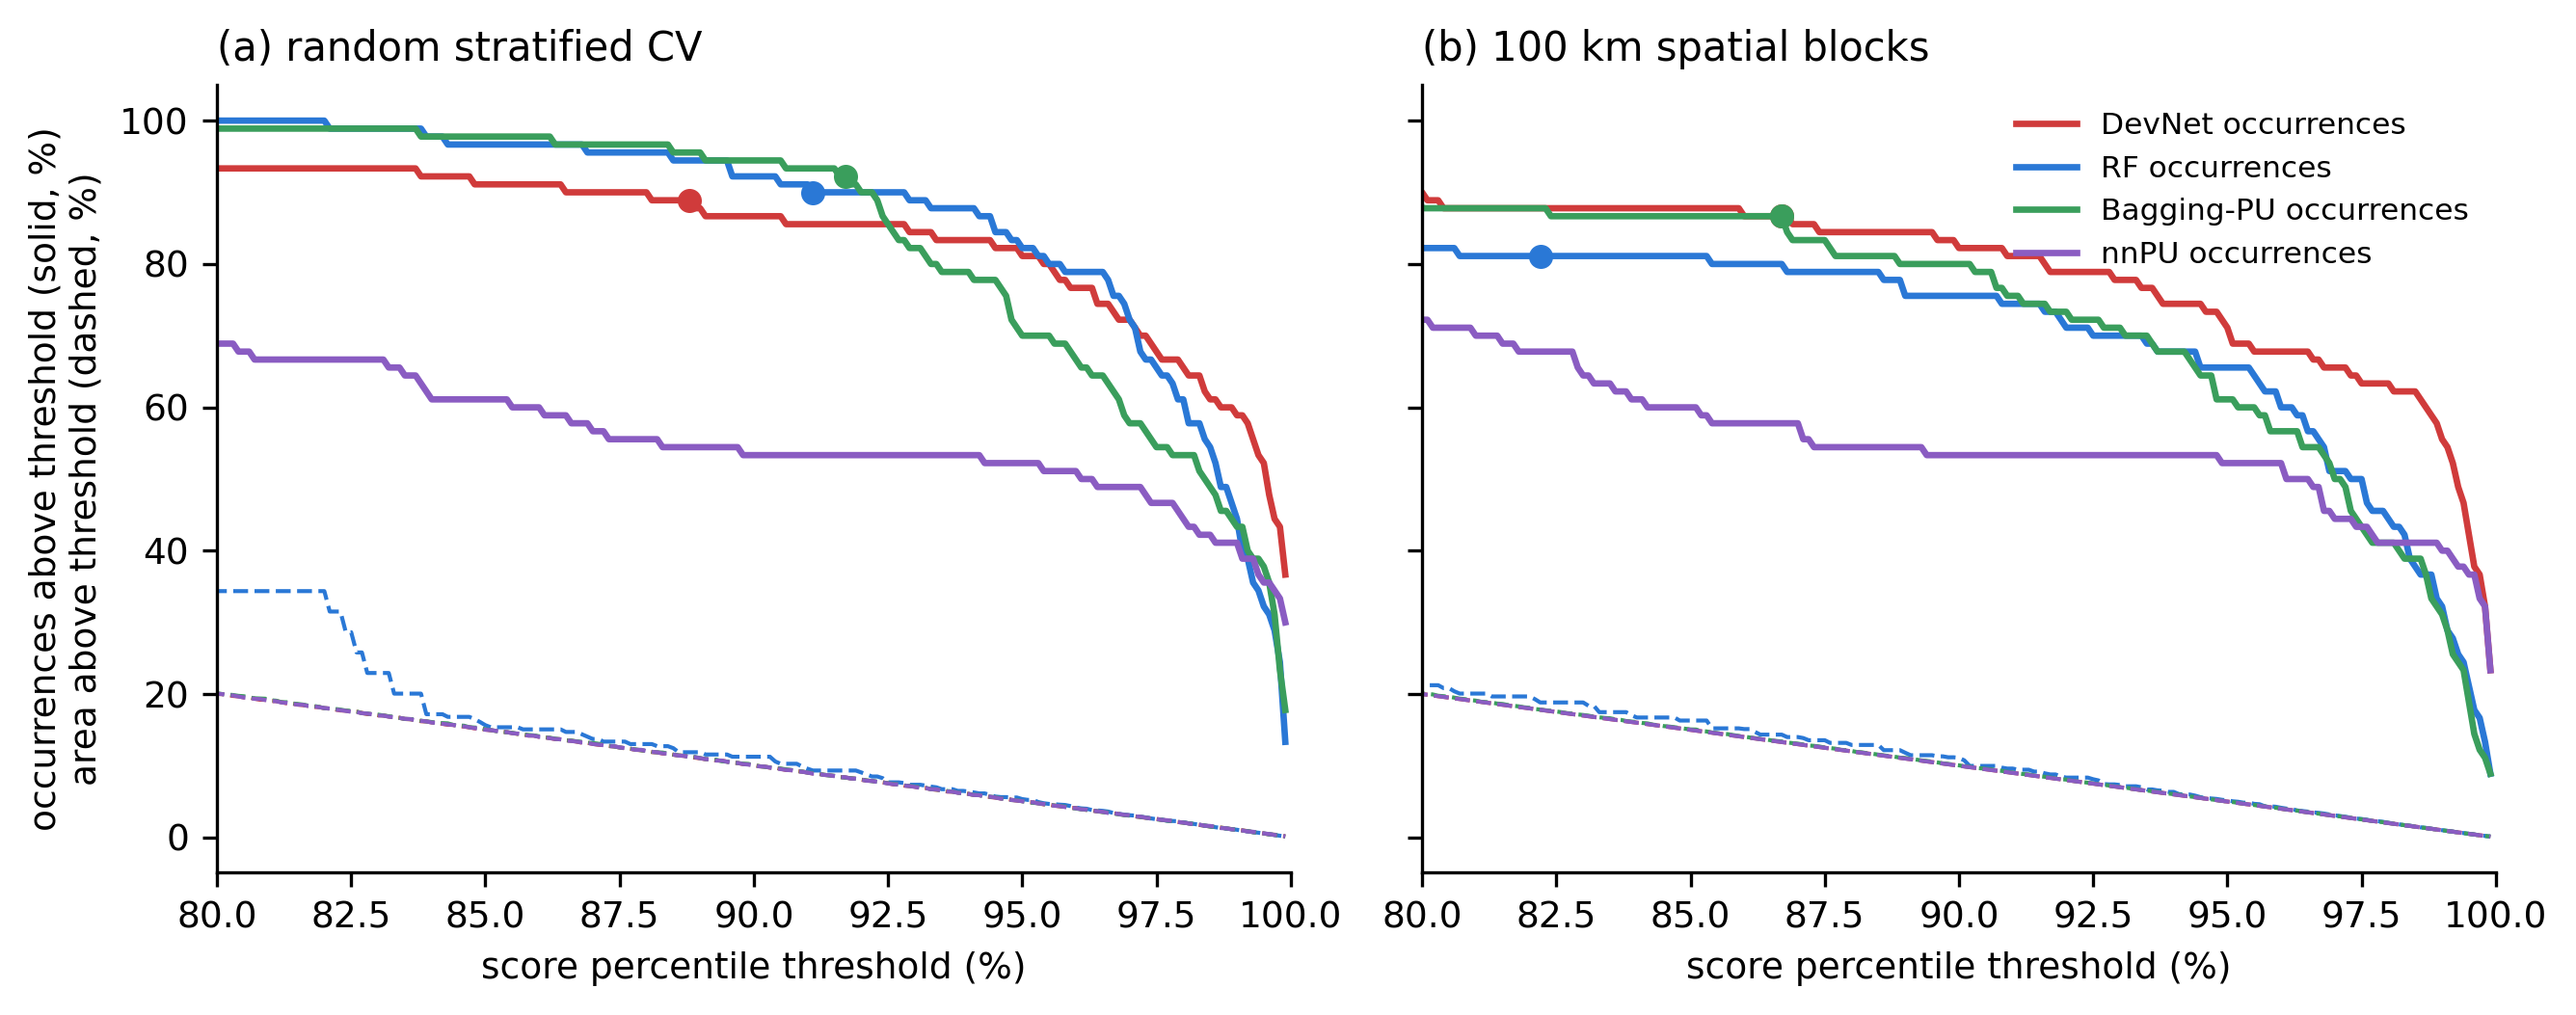
\includegraphics[width=0.9\textwidth]{figures/fig_pa_superior_rev.png}
\caption{Prediction--area curves for Superior from out-of-fold ranks: share of held-out occurrences (solid) and of the evaluation background, a proxy for area (dashed), above a score-percentile threshold; dots mark the intersections. (a) Random cross-validation, (b) 100~km spatial blocks.}\label{fig:pa}
\end{figure}

\begin{table}[!h]
\caption{As Table~\ref{tab:benchmark}, for the full 48-feature set.}\label{tab:benchmark-full}
\footnotesize
\begin{tabular*}{\textwidth}{@{\extracolsep\fill}llcc}
\toprule
Region ($n_{\mathrm{pos}}$) & Model & AUC & AP \\
\midrule
\multirow{5}{*}{Superior (15)} & DevNet & 0.938 [0.921, 0.954] & \textbf{0.351} [0.252, 0.428] \\
 & RF & \textbf{0.969} [0.878, 0.978] & 0.222 [0.170, 0.273] \\
 & Bagging-PU & 0.940 [0.922, 0.958] & 0.187 [0.160, 0.224] \\
 & nnPU & 0.829 [0.827, 0.838] & 0.268 [0.218, 0.283] \\
 & RF (fixed seed) & 0.961 [0.917, 0.984] & 0.222 [0.181, 0.276] \\
\midrule
\multirow{5}{*}{Cordillera (27)} & DevNet & 0.859 [0.830, 0.889] & 0.166 [0.116, 0.203] \\
 & RF & \textbf{0.909} [0.887, 0.923] & \textbf{0.379} [0.262, 0.433] \\
 & Bagging-PU & 0.895 [0.890, 0.911] & 0.339 [0.249, 0.370] \\
 & nnPU & 0.515 [0.490, 0.526] & 0.013 [0.011, 0.014] \\
 & RF (fixed seed) & 0.905 [0.883, 0.932] & 0.369 [0.299, 0.439] \\
\midrule
\multirow{5}{*}{Grenville (12)} & DevNet & \textbf{0.800} [0.755, 0.831] & 0.180 [0.106, 0.213] \\
 & RF & 0.799 [0.748, 0.860] & \textbf{0.218} [0.102, 0.392] \\
 & Bagging-PU & 0.772 [0.752, 0.821] & 0.132 [0.080, 0.244] \\
 & nnPU & 0.655 [0.632, 0.671] & 0.009 [0.007, 0.010] \\
 & RF (fixed seed) & 0.867 [0.794, 0.897] & 0.203 [0.144, 0.334] \\
\botrule
\end{tabular*}
\end{table}

\begin{table}[!h]
\caption{AUC (median over six repeats) for the runs of Table~\ref{tab:spatial}. Bold: highest AUC in each row.}\label{tab:spatial-auc}
\footnotesize
\setlength{\tabcolsep}{3pt}
\begin{tabular*}{\textwidth}{@{\extracolsep\fill}llcccc}
\toprule
Region & Split & DevNet & RF & Bagging-PU & nnPU \\
\midrule
\multirow{4}{*}{Superior} & random & 0.951 & \textbf{0.973} & 0.969 & 0.835 \\
 & 50 km blocks & 0.944 & 0.933 & \textbf{0.954} & 0.829 \\
 & 100 km blocks & \textbf{0.939} & 0.900 & 0.917 & 0.829 \\
 & 200 km blocks & 0.834 & \textbf{0.879} & 0.870 & 0.819 \\
\midrule
\multirow{4}{*}{Cordillera} & random & 0.873 & 0.904 & \textbf{0.912} & 0.574 \\
 & 50 km blocks & 0.800 & 0.782 & \textbf{0.853} & 0.580 \\
 & 100 km blocks & 0.586 & 0.650 & \textbf{0.775} & 0.556 \\
 & 200 km blocks & 0.607 & 0.625 & \textbf{0.746} & 0.556 \\
\midrule
\multirow{4}{*}{Grenville} & random & 0.770 & 0.837 & \textbf{0.842} & 0.597 \\
 & 50 km blocks & 0.661 & 0.707 & \textbf{0.714} & 0.564 \\
 & 100 km blocks & 0.634 & 0.621 & \textbf{0.673} & 0.579 \\
 & 200 km blocks & 0.572 & \textbf{0.602} & 0.555 & 0.562 \\
\botrule
\end{tabular*}
\end{table}

\section{Augmentation under spatially blocked validation}\label{app:aug-spatial}

\begin{table}[!h]
\caption{Superior average precision with fold-safe synthetic positives under spatially blocked cross-validation (median and 95\% interval over six repeats), with the paired per-repeat difference from no augmentation.}\label{tab:aug-spatial}
\footnotesize
\begin{tabular*}{\textwidth}{@{\extracolsep\fill}lllccc}
\toprule
Blocks & Model & Augmentation & AP & $\Delta$AP per repeat & wins \\
\midrule
100 km & DevNet & none & 0.302 [0.225, 0.349] & -- & -- \\
 &  & Gaussian jitter 10$\times$ & 0.334 [0.223, 0.349] & +0.005 [-0.003, +0.058] & 4/6 \\
 &  & SMOTE 3$\times$ & 0.301 [0.222, 0.413] & +0.000 [-0.042, +0.132] & 3/6 \\
 &  & WGAN-GP 3$\times$ & 0.310 [0.247, 0.424] & +0.007 [-0.022, +0.147] & 3/6 \\
 &  & WGAN-GP 10$\times$ & 0.298 [0.234, 0.362] & +0.004 [-0.074, +0.076] & 3/6 \\
\addlinespace
100 km & RF & none & 0.128 [0.049, 0.190] & -- & -- \\
 &  & Gaussian jitter 10$\times$ & 0.130 [0.067, 0.222] & +0.006 [-0.061, +0.081] & 5/6 \\
 &  & SMOTE 3$\times$ & 0.095 [0.043, 0.215] & -0.007 [-0.116, +0.084] & 2/6 \\
 &  & WGAN-GP 3$\times$ & 0.159 [0.062, 0.253] & +0.031 [+0.007, +0.106] & 6/6 \\
 &  & WGAN-GP 10$\times$ & 0.161 [0.083, 0.239] & +0.040 [-0.019, +0.094] & 5/6 \\
\addlinespace
200 km & DevNet & none & 0.341 [0.197, 0.388] & -- & -- \\
 &  & Gaussian jitter 10$\times$ & 0.356 [0.220, 0.413] & +0.010 [+0.001, +0.126] & 6/6 \\
 &  & SMOTE 3$\times$ & 0.330 [0.234, 0.362] & -0.006 [-0.043, +0.062] & 2/6 \\
 &  & WGAN-GP 3$\times$ & 0.355 [0.270, 0.376] & +0.012 [-0.015, +0.119] & 5/6 \\
 &  & WGAN-GP 10$\times$ & 0.366 [0.270, 0.421] & +0.041 [-0.010, +0.150] & 4/6 \\
\addlinespace
200 km & RF & none & 0.094 [0.036, 0.150] & -- & -- \\
 &  & Gaussian jitter 10$\times$ & 0.079 [0.053, 0.122] & -0.025 [-0.067, +0.045] & 2/6 \\
 &  & SMOTE 3$\times$ & 0.094 [0.052, 0.112] & +0.008 [-0.058, +0.023] & 4/6 \\
 &  & WGAN-GP 3$\times$ & 0.118 [0.075, 0.154] & +0.012 [-0.036, +0.076] & 3/6 \\
 &  & WGAN-GP 10$\times$ & 0.094 [0.060, 0.153] & +0.008 [-0.053, +0.072] & 3/6 \\
\botrule
\end{tabular*}
\end{table}

\section{Interpretation in the contrasting provinces}\label{app:shap}

\begin{table}[!h]
\caption{As Table~\ref{tab:shap}, Cordillera (33 features).}\label{tab:shap-cord}
\footnotesize
\begin{tabular*}{\textwidth}{@{\extracolsep\fill}lcccc}
\toprule
Feature & DevNet rank & DevNet dir. & RF rank & RF dir. \\
\midrule
Era: Mesozoic & 1 & $\downarrow$ (-0.82) & 8 & $\downarrow$ (-0.82) \\
Bouguer anomaly (BA) & 3 & $\downarrow$ (-0.97) & 2 & $\downarrow$ (-0.87) \\
Passive-margin proximity & 22 & $\uparrow$ (+0.94) & 1 & $\uparrow$ (+0.56) \\
Era: Proterozoic & 2 & $\uparrow$ (+0.73) & 14 & $\uparrow$ (+0.74) \\
Moho depth & 4 & $\uparrow$ (+0.97) & 6 & $\uparrow$ (+0.83) \\
Fault proximity & 5 & $\uparrow$ (+0.94) & 7 & $\uparrow$ (+0.87) \\
Deep-source RTP & 17 & $\downarrow$ (-0.96) & 3 & $\downarrow$ (-0.75) \\
Gravity up-cont. 30 km HGM & 18 & $\uparrow$ (+0.93) & 4 & $\uparrow$ (+0.84) \\
Deep magnetic-worm proximity & 16 & $\downarrow$ (-0.95) & 5 & $\downarrow$ (-0.87) \\
BA high-pass 40 km GLCM contrast & 11 & $\downarrow$ (-0.95) & 10 & $\downarrow$ (-0.31) \\
\botrule
\end{tabular*}
\end{table}

\begin{table}[!h]
\caption{As Table~\ref{tab:shap}, Grenville (33 features).}\label{tab:shap-gren}
\footnotesize
\begin{tabular*}{\textwidth}{@{\extracolsep\fill}lcccc}
\toprule
Feature & DevNet rank & DevNet dir. & RF rank & RF dir. \\
\midrule
Deep-source RTP & 1 & $\uparrow$ (+0.99) & 1 & $\uparrow$ (+0.74) \\
BA high-pass 40 km GLCM contrast & 2 & $\uparrow$ (+0.99) & 3 & $\uparrow$ (+0.86) \\
DRTP THD tilt & 6 & $\downarrow$ (-0.99) & 2 & $\downarrow$ (-0.80) \\
Deep gravity-worm proximity & 5 & $\uparrow$ (+0.99) & 9 & $\uparrow$ (+0.82) \\
Bouguer anomaly (BA) GLCM energy & 4 & $\uparrow$ (+0.93) & 16 & $\uparrow$ (+0.94) \\
Moho depth & 13 & $\downarrow$ (-0.97) & 4 & $\downarrow$ (-0.71) \\
Era: Proterozoic & 3 & $\downarrow$ (-0.63) & 27 & $\downarrow$ (-0.63) \\
Deep magnetic-worm proximity & 8 & $\uparrow$ (+0.99) & 13 & $\uparrow$ (+0.73) \\
DRTP & 12 & $\uparrow$ (+0.98) & 6 & $\uparrow$ (+0.59) \\
DRTP 1VD & 7 & $\downarrow$ (-0.99) & 22 & $\downarrow$ (-0.91) \\
\botrule
\end{tabular*}
\end{table}

\section{Ablation of DevNet design choices}\label{app:sensitivity}

DevNet's two design choices (Section~\ref{sec:models}) were settled with diagnostic experiments on the three provinces of this study, by changing one element at a time from a configuration with z-scored inputs and label-balanced batches of 16 + 16 rows. Each configuration in Table~\ref{tab:ablation} was fixed before it was run and was not tuned afterwards, and all are evaluated with the folds, protocols and seeds of the main results. The nested early-stopping configuration chooses the number of steps (100--3,000, cosine schedule over 3,000 steps) inside each outer training fold by a 100~km spatial cross-validation (three inner folds, two inner restarts, background purged from inner validation blocks), so the test fold is never used for the choice. Table~\ref{tab:margin} gives the sensitivity of the final configuration to the deviation margin.

\begin{table}[!h]
\caption{Ablation of DevNet's design choices: AP (median over six repeats) under random cross-validation and spatial blocks, on identical folds. Inputs: quantile-normal or z-scored; batch: positive\,+\,background rows per step; steps: number of gradient steps (nested ES: chosen by nested 100~km spatial cross-validation). In brackets: number of repeats in which the final configuration (bold) has the higher AP. --: not run.}\label{tab:ablation}
\scriptsize
\setlength{\tabcolsep}{2.5pt}
\begin{tabular*}{\textwidth}{@{\extracolsep\fill}llllllll}
\toprule
Region & Inputs & Batch & Steps & random & 50 km & 100 km & 200 km \\
\midrule
\multirow{6}{*}{Superior} & quantile & 16\,+\,240 & 300 (final) & \textbf{0.354} & \textbf{0.322} & \textbf{0.302} & \textbf{0.341} \\
 & z-score & 16\,+\,240 & 300 & 0.280 (5/6) & 0.298 (6/6) & 0.244 (4/6) & 0.244 (4/6) \\
 & quantile & 16\,+\,16 & 300 & 0.328 (3/6) & 0.322 (2/6) & 0.278 (3/6) & 0.308 (2/6) \\
 & z-score & 16\,+\,16 & 300 & 0.272 (5/6) & 0.239 (6/6) & 0.209 (5/6) & 0.235 (5/6) \\
 & z-score & 16\,+\,16 & 3,000 & 0.305 (5/6) & -- & 0.190 (5/6) & -- \\
 & z-score & 16\,+\,16 & nested ES & 0.283 (6/6) & 0.236 (6/6) & 0.228 (5/6) & 0.222 (5/6) \\
\midrule
\multirow{6}{*}{Cordillera} & quantile & 16\,+\,240 & 300 (final) & \textbf{0.136} & \textbf{0.042} & \textbf{0.021} & \textbf{0.018} \\
 & z-score & 16\,+\,240 & 300 & 0.122 (6/6) & 0.058 (4/6) & 0.018 (2/6) & 0.020 (3/6) \\
 & quantile & 16\,+\,16 & 300 & 0.128 (6/6) & 0.044 (4/6) & 0.019 (2/6) & 0.018 (2/6) \\
 & z-score & 16\,+\,16 & 300 & 0.113 (6/6) & 0.054 (4/6) & 0.021 (1/6) & 0.024 (2/6) \\
 & z-score & 16\,+\,16 & 3,000 & 0.159 (2/6) & -- & 0.012 (5/6) & -- \\
 & z-score & 16\,+\,16 & nested ES & 0.127 (4/6) & 0.067 (4/6) & 0.015 (2/6) & 0.015 (6/6) \\
\midrule
\multirow{6}{*}{Grenville} & quantile & 16\,+\,240 & 300 (final) & \textbf{0.137} & \textbf{0.037} & \textbf{0.008} & \textbf{0.007} \\
 & z-score & 16\,+\,240 & 300 & 0.049 (6/6) & 0.015 (6/6) & 0.005 (6/6) & 0.005 (6/6) \\
 & quantile & 16\,+\,16 & 300 & 0.113 (6/6) & 0.033 (5/6) & 0.008 (5/6) & 0.007 (5/6) \\
 & z-score & 16\,+\,16 & 300 & 0.040 (6/6) & 0.012 (6/6) & 0.005 (6/6) & 0.004 (6/6) \\
 & z-score & 16\,+\,16 & 3,000 & 0.067 (5/6) & -- & 0.006 (5/6) & -- \\
 & z-score & 16\,+\,16 & nested ES & 0.064 (5/6) & 0.019 (6/6) & 0.005 (5/6) & 0.005 (5/6) \\
\botrule
\end{tabular*}
\end{table}

\begin{table}[!h]
\caption{Sensitivity of DevNet to the deviation margin $a$ (AP, median over six repeats, random cross-validation). The main results use $a = 5$.}\label{tab:margin}
\footnotesize
\begin{tabular*}{0.7\textwidth}{@{\extracolsep\fill}lcccc}
\toprule
Region & $a = 2$ & $a = 3$ & $a = 5$ & $a = 8$ \\
\midrule
Superior & 0.360 & 0.362 & 0.354 & 0.360 \\
Cordillera & 0.197 & 0.173 & 0.136 & 0.120 \\
Grenville & 0.154 & 0.129 & 0.137 & 0.114 \\
\botrule
\end{tabular*}
\end{table}

\end{appendices}

\clearpage

\bibliography{references}

\end{document}
